\documentclass[12pt,a4paper]{article}
\usepackage[utf8]{inputenc}
\usepackage[T1]{fontenc}
\usepackage[brazilian]{babel}
\usepackage{geometry}
\usepackage{graphicx}
\usepackage{amsmath,amssymb}
\usepackage{float}
\usepackage{setspace}
\usepackage{indentfirst}
\usepackage{array}
\usepackage{longtable}
\usepackage{caption}
\usepackage{textcomp}
\usepackage[hidelinks]{hyperref}

% Fonte Arial (Helvetica/Nimbus Sans, equivalente metrico da Arial) e texto todo preto
\usepackage[scaled=0.95]{helvet}
\renewcommand{\familydefault}{\sfdefault}
\captionsetup{font=small,labelfont=bf,labelsep=endash}
\captionsetup[table]{position=top}

\geometry{top=3cm, bottom=2cm, left=3cm, right=2cm}

\onehalfspacing
\setlength{\emergencystretch}{3em}   % evita linhas estouradas com nomes de arquivos longos
% permite quebrar linha depois de "_" (nomes de arquivos longos)
\DeclareRobustCommand{\_}{\textunderscore\allowbreak}
\setlength{\LTpre}{6pt}
\setlength{\LTpost}{6pt}

\begin{document}


\begin{titlepage}
    \centering

    % Logo da Universidade
    
\includegraphics[width=3.5cm]{Imagens/ufam-logo.jpg}\\[1cm]

    {\large \textbf{UNIVERSIDADE FEDERAL DO AMAZONAS -- UFAM}} \\[0.3cm]
    {\large \textbf{PROGRAMA DE PÓS-GRADUAÇÃO EM ENGENHARIA ELÉTRICA -- PPGEE}} \\[0.3cm]
    {\large \textbf{Disciplina: Tópicos em Redes Móveis}} \\[2cm]

    {\Large \textbf{Trabalho Final -- Parte 1: Análise dos Sinais de CSI e Geração de Dados Sintéticos por EEMD}} \\[2cm]

    \begin{flushleft}
        \textbf{Equipe 12} \\[0.3cm]
        \textbf{Autores:} \\
        André Ramos Costa \\
        John Deyvy Correa Guedes \\
        Luca Dias Naja \\
        Matheus Serrão Uchoa \\
        Renan Barroncas Silva \\[0.5cm]

        \textbf{Participantes da base analisados:} s12, s13 e s14 \\[1cm]

        \textbf{Professor:} \\
        Dr. Celso Barbosa Carvalho
    \end{flushleft}

    \vfill

    {\large Manaus -- AM} \\
    {\large \the\year}
\end{titlepage}


\newpage
\tableofcontents
\newpage


\section{Objetivo}

Este trabalho analisa as amplitudes de \textit{Channel State Information} (CSI) de cinco atividades humanas - FA (queda), GU (levantar-se), LD (deitar-se), SD (sentar-se) e WA (caminhar) - da base disponibilizada com o artigo \textit{Tools and Methods for Achieving Wi-Fi Sensing in Embedded Devices} (Armenta-Garcia et al., Sensors 2025). Os objetivos são: (i) inventariar e verificar as gravações; (ii) selecionar 30 gravações dos participantes atribuídos à equipe; (iii) calcular e visualizar as amplitudes de CSI; (iv) resumir a amplitude do par 20 por cinco características estatísticas; e (v) gerar sinais sintéticos por EEMD, recombinando componentes de duas gravações reais, e compará-los com os sinais de origem.

\subsection{Materiais e reprodução}

Todo o processamento foi feito pelo programa \textbf{analise\_csi.py}, que executa as seções 1 a 5 em sequência e gera os CSV, as figuras e o arquivo de sinais sintéticos. O caminho da base e o ID da equipe são configurados no topo do arquivo; as instruções completas estão no LEIA-ME.txt. Ambiente utilizado: Python 3.10.11, numpy 1.26.4, pandas 2.2.2, matplotlib 3.10.9 e EMD-signal (PyEMD) 1.10.0. Os cálculos foram validados com os exemplos do enunciado: para Datasets/Activity/FA/s1/csi\_data\_1720464506.txt o código reproduz a amplitude 16,28 do par 20 no registro 1 e a média 21,5859, o desvio padrão 4,4086 e o pico a pico 29,0998 da série do par 20; para a série [2, 5, 3, 8] obtém pico a pico 6 e média das diferenças absolutas 3,33.

\section{Organização e verificação das gravações (seção 1)}

\subsection{Procedimento}

O programa percorre Datasets/Activity/\{FA, GU, LD, SD, WA\}/s*/ e lê todos os arquivos csi\_data\_*.txt (a pasta Breathing(experimental), os modelos e os arquivos NPY não são considerados). Cada TXT é lido linha a linha: \textbf{total\_registros} conta as linhas não vazias, e \textbf{registros\_formato\_valido} conta as linhas com exatamente 129 valores numéricos finitos separados por vírgula (1 valor temporal + 64 pares imaginária/real). Linhas com outra quantidade de valores, valores não numéricos ou não finitos são descritas na coluna \textbf{problemas\_leitura} com o número da linha e o motivo. O resultado está em \textbf{inventario\_gravacoes.csv} (uma linha por TXT).

\subsection{Resultados}

Foram encontrados \textbf{1647 arquivos TXT}, com 1.623.376 registros (linhas não vazias) no total, todos com formato válido: nenhum arquivo apresentou linha vazia intermediária, falha de leitura ou linha fora do formato de 129 valores. A quantidade de registros por gravação varia de 866 a 1001 (mediana 988), o que é compatível com a coleta descrita no artigo (cerca de 50 pacotes por segundo durante 20 s por repetição). Essa variação não caracteriza erro.

{\footnotesize
\begin{longtable}{|>{\centering\arraybackslash}p{2.49cm}|>{\centering\arraybackslash}p{1.73cm}|>{\centering\arraybackslash}p{1.73cm}|>{\centering\arraybackslash}p{1.73cm}|>{\centering\arraybackslash}p{1.73cm}|>{\centering\arraybackslash}p{1.73cm}|>{\centering\arraybackslash}p{1.73cm}|}
\caption{Quantidade de arquivos TXT (gravações) por participante e atividade. Cada célula conta arquivos, não registros dentro de um TXT. Fonte: contagem\_gravacoes.csv.}\\
\hline
\textbf{Participante} & \textbf{FA} & \textbf{GU} & \textbf{LD} & \textbf{SD} & \textbf{WA} & \textbf{Total} \\ \hline
\endfirsthead
\hline
\textbf{Participante} & \textbf{FA} & \textbf{GU} & \textbf{LD} & \textbf{SD} & \textbf{WA} & \textbf{Total} \\ \hline
\endhead
s1 & 14 & 15 & 15 & 15 & 15 & 74 \\ \hline
s2 & 15 & 15 & 15 & 15 & 15 & 75 \\ \hline
s3 & 15 & 15 & 15 & 15 & 15 & 75 \\ \hline
s4 & 15 & 15 & 15 & 15 & 15 & 75 \\ \hline
s5 & 15 & 14 & 15 & 15 & 15 & 74 \\ \hline
s6 & 15 & 15 & 15 & 15 & 15 & 75 \\ \hline
s7 & 14 & 15 & 15 & 15 & 15 & 74 \\ \hline
s8 & 15 & 15 & 15 & 15 & 15 & 75 \\ \hline
s9 & 15 & 15 & 15 & 15 & 16 & 76 \\ \hline
s10 & 15 & 15 & 15 & 15 & 15 & 75 \\ \hline
s11 & 15 & 15 & 15 & 15 & 15 & 75 \\ \hline
s12 & 15 & 14 & 14 & 16 & 15 & 74 \\ \hline
s13 & 15 & 15 & 15 & 15 & 15 & 75 \\ \hline
s14 & 15 & 15 & 15 & 16 & 14 & 75 \\ \hline
s15 & 15 & 15 & 15 & 15 & 15 & 75 \\ \hline
s16 & 14 & 15 & 15 & 15 & 15 & 74 \\ \hline
s17 & 15 & 15 & 15 & 15 & 15 & 75 \\ \hline
s19 & 15 & 16 & 16 & 15 & 15 & 77 \\ \hline
s21 & 15 & 15 & 15 & 15 & 15 & 75 \\ \hline
s22 & 15 & 15 & 15 & 15 & 15 & 75 \\ \hline
s23 & 15 & 15 & 15 & 15 & 15 & 75 \\ \hline
s24 & 15 & 15 & 14 & 15 & 15 & 74 \\ \hline
\textbf{Total} & \textbf{327} & \textbf{329} & \textbf{329} & \textbf{332} & \textbf{330} & \textbf{1647} \\ \hline
\end{longtable}
}

\subsection{Comparação com o artigo}

O artigo informa 22 voluntários, cada um realizando 15 repetições de cinco atividades, e um total de 1.647 amostras coletadas. A contagem obtida coincide com esses números: \textbf{1.647 gravações} e \textbf{22 participantes}. Observações sobre a diferença entre o desenho do experimento e a base:

\begin{itemize}
    \item 22 × 5 × 15 = 1.650 gravações seriam esperadas. A base tem 8 combinações participante/atividade com 14 arquivos (s1/FA, s5/GU, s7/FA, s12/GU, s12/LD, s14/WA, s16/FA, s24/LD) e 5 com 16 arquivos (s9/WA, s12/SD, s14/SD, s19/GU, s19/LD); 1.650 - 8 + 5 = 1.647.
    \item Existem 22 pastas de participantes em cada atividade, e as 22 possuem gravações nas cinco atividades (não há pasta vazia). A numeração, porém, não é contínua: os identificadores \textbf{s18 e s20 não existem} na base, de modo que os participantes vão de s1 a s24 com duas lacunas. Vale notar que o script dos autores Scripts/imf\_generator.py lista s18 entre os participantes, embora essa pasta não exista.
    \item Nenhuma gravação foi excluída por erro de formato, portanto a base analisada corresponde integralmente à informada no artigo.
\end{itemize}

\section{Seleção das 30 gravações (seção 2)}

\textbf{Equipe 12 - participantes da base: s12, s13 e s14.} Para cada participante e atividade, os nomes dos TXT foram ordenados em ordem crescente e foram selecionados os dois primeiros arquivos que, segundo o inventário, podem ser lidos e têm todas as linhas não vazias no formato de 129 valores numéricos finitos. A seleção completa (30 linhas) está em \textbf{selecao\_30\_gravacoes.csv}, com as colunas participante, atividade, caminho\_txt, ordem\_selecao e n\_registros.

\textbf{Arquivos desconsiderados:} nenhum. Os dois primeiros TXT de cada uma das 15 combinações participante/atividade estavam íntegros, portanto não houve substituição. A Tabela 2 resume a seleção.

{\footnotesize
\begin{longtable}{|>{\centering\arraybackslash}p{1.88cm}|>{\centering\arraybackslash}p{1.71cm}|>{\centering\arraybackslash}p{5.30cm}|>{\centering\arraybackslash}p{5.30cm}|}
\caption{Gravações selecionadas (caminho completo: Datasets/Activity/\textless{}atividade\textgreater{}/\textless{}participante\textgreater{}/\textless{}arquivo\textgreater{}).}\\
\hline
\textbf{Participante} & \textbf{Atividade} & \textbf{ordem\_selecao = 1 (registros)} & \textbf{ordem\_selecao = 2 (registros)} \\ \hline
\endfirsthead
\hline
\textbf{Participante} & \textbf{Atividade} & \textbf{ordem\_selecao = 1 (registros)} & \textbf{ordem\_selecao = 2 (registros)} \\ \hline
\endhead
s12 & FA & csi\_data\_1722274497.txt (974) & csi\_data\_1722274542.txt (963) \\ \hline
s12 & GU & csi\_data\_1722275364.txt (987) & csi\_data\_1722275473.txt (990) \\ \hline
s12 & LD & csi\_data\_1722275315.txt (991) & csi\_data\_1722275426.txt (936) \\ \hline
s12 & SD & csi\_data\_1722273691.txt (976) & csi\_data\_1722273739.txt (978) \\ \hline
s12 & WA & csi\_data\_1722272856.txt (995) & csi\_data\_1722272903.txt (994) \\ \hline
s13 & FA & csi\_data\_1722285593.txt (987) & csi\_data\_1722285652.txt (978) \\ \hline
s13 & GU & csi\_data\_1722281824.txt (962) & csi\_data\_1722281947.txt (986) \\ \hline
s13 & LD & csi\_data\_1722281718.txt (979) & csi\_data\_1722281887.txt (983) \\ \hline
s13 & SD & csi\_data\_1722286503.txt (992) & csi\_data\_1722286550.txt (991) \\ \hline
s13 & WA & csi\_data\_1722284702.txt (982) & csi\_data\_1722284759.txt (975) \\ \hline
s14 & FA & csi\_data\_1722360030.txt (974) & csi\_data\_1722360079.txt (992) \\ \hline
s14 & GU & csi\_data\_1722361809.txt (986) & csi\_data\_1722361907.txt (994) \\ \hline
s14 & LD & csi\_data\_1722361762.txt (983) & csi\_data\_1722361861.txt (990) \\ \hline
s14 & SD & csi\_data\_1722360869.txt (989) & csi\_data\_1722360914.txt (977) \\ \hline
s14 & WA & csi\_data\_1722359256.txt (991) & csi\_data\_1722359307.txt (980) \\ \hline
\end{longtable}
}

\newpage

\section{Amplitudes de CSI (seção 3)}

\subsection{Cálculo}

Em cada linha de cada TXT, a primeira coluna (informação temporal) é separada e os 128 valores restantes são agrupados em 64 pares (imaginária, real), nessa ordem. A amplitude de cada par é |H| = (Re(H)\textsuperscript{2} + Im(H)\textsuperscript{2})\textsuperscript{1/2}, como na função get\_amps de Scripts/CSI.py. Cada TXT gera uma matriz com uma linha por registro e 64 colunas; por exemplo, o arquivo csi\_data\_1722274497.txt (s12, FA, 974 registros) gera uma matriz 974 × 64. As amplitudes foram calculadas para os 30 arquivos selecionados.

\subsection{Verificação numérica do par 20}

{\footnotesize
\begin{longtable}{|>{\centering\arraybackslash}p{4.03cm}|>{\centering\arraybackslash}p{1.45cm}|>{\centering\arraybackslash}p{0.89cm}|>{\centering\arraybackslash}p{2.26cm}|>{\centering\arraybackslash}p{1.93cm}|>{\centering\arraybackslash}p{2.74cm}|}
\caption{Verificação do cálculo da amplitude (gravação s12/FA, ordem\_selecao = 1).}\\
\hline
\textbf{TXT} & \textbf{Linha do TXT} & \textbf{Par} & \textbf{Imaginária (coluna 40)} & \textbf{Real (coluna 41)} & \textbf{Amplitude (coluna 20 da matriz)} \\ \hline
\endfirsthead
\hline
\textbf{TXT} & \textbf{Linha do TXT} & \textbf{Par} & \textbf{Imaginária (coluna 40)} & \textbf{Real (coluna 41)} & \textbf{Amplitude (coluna 20 da matriz)} \\ \hline
\endhead
csi\_data\_1722274497.txt (s12, FA) & 1 & 20 & 33 & 5 & 33,38 \\ \hline
\end{longtable}
}

Conferência: (5\textsuperscript{2} + 33\textsuperscript{2})\textsuperscript{1/2} = 1114\textsuperscript{1/2} = 33,38, igual ao valor da coluna 20 da matriz de amplitudes e ao primeiro ponto da série temporal da Figura 1 (s12) e à célula registro 1 / par 20 do mapa de calor correspondente.

\subsection{Painéis por atividade}

Para cada participante e atividade foi usada a gravação com ordem\_selecao = 1 (15 gravações). Cada painel (Figuras 1 a 5) mostra, na linha superior, a série temporal da amplitude do par 20 de s12, s13 e s14 e, na linha inferior, o mapa de calor dos 64 pares. O eixo horizontal é o índice do registro (a partir de 1), não o tempo em segundos. As 15 séries usam os mesmos limites (0 a 51,4) e os 15 mapas usam a mesma escala de cores (0 a 115,3, percentil 99,5 de todas as amplitudes). O par 1 tem amplitude constante de cerca de 115 e o máximo absoluto chega a 159,5; por isso a barra de cores indica saturação (seta) para não comprimir a escala dos demais pares.

\begin{figure}[H]
    \centering
    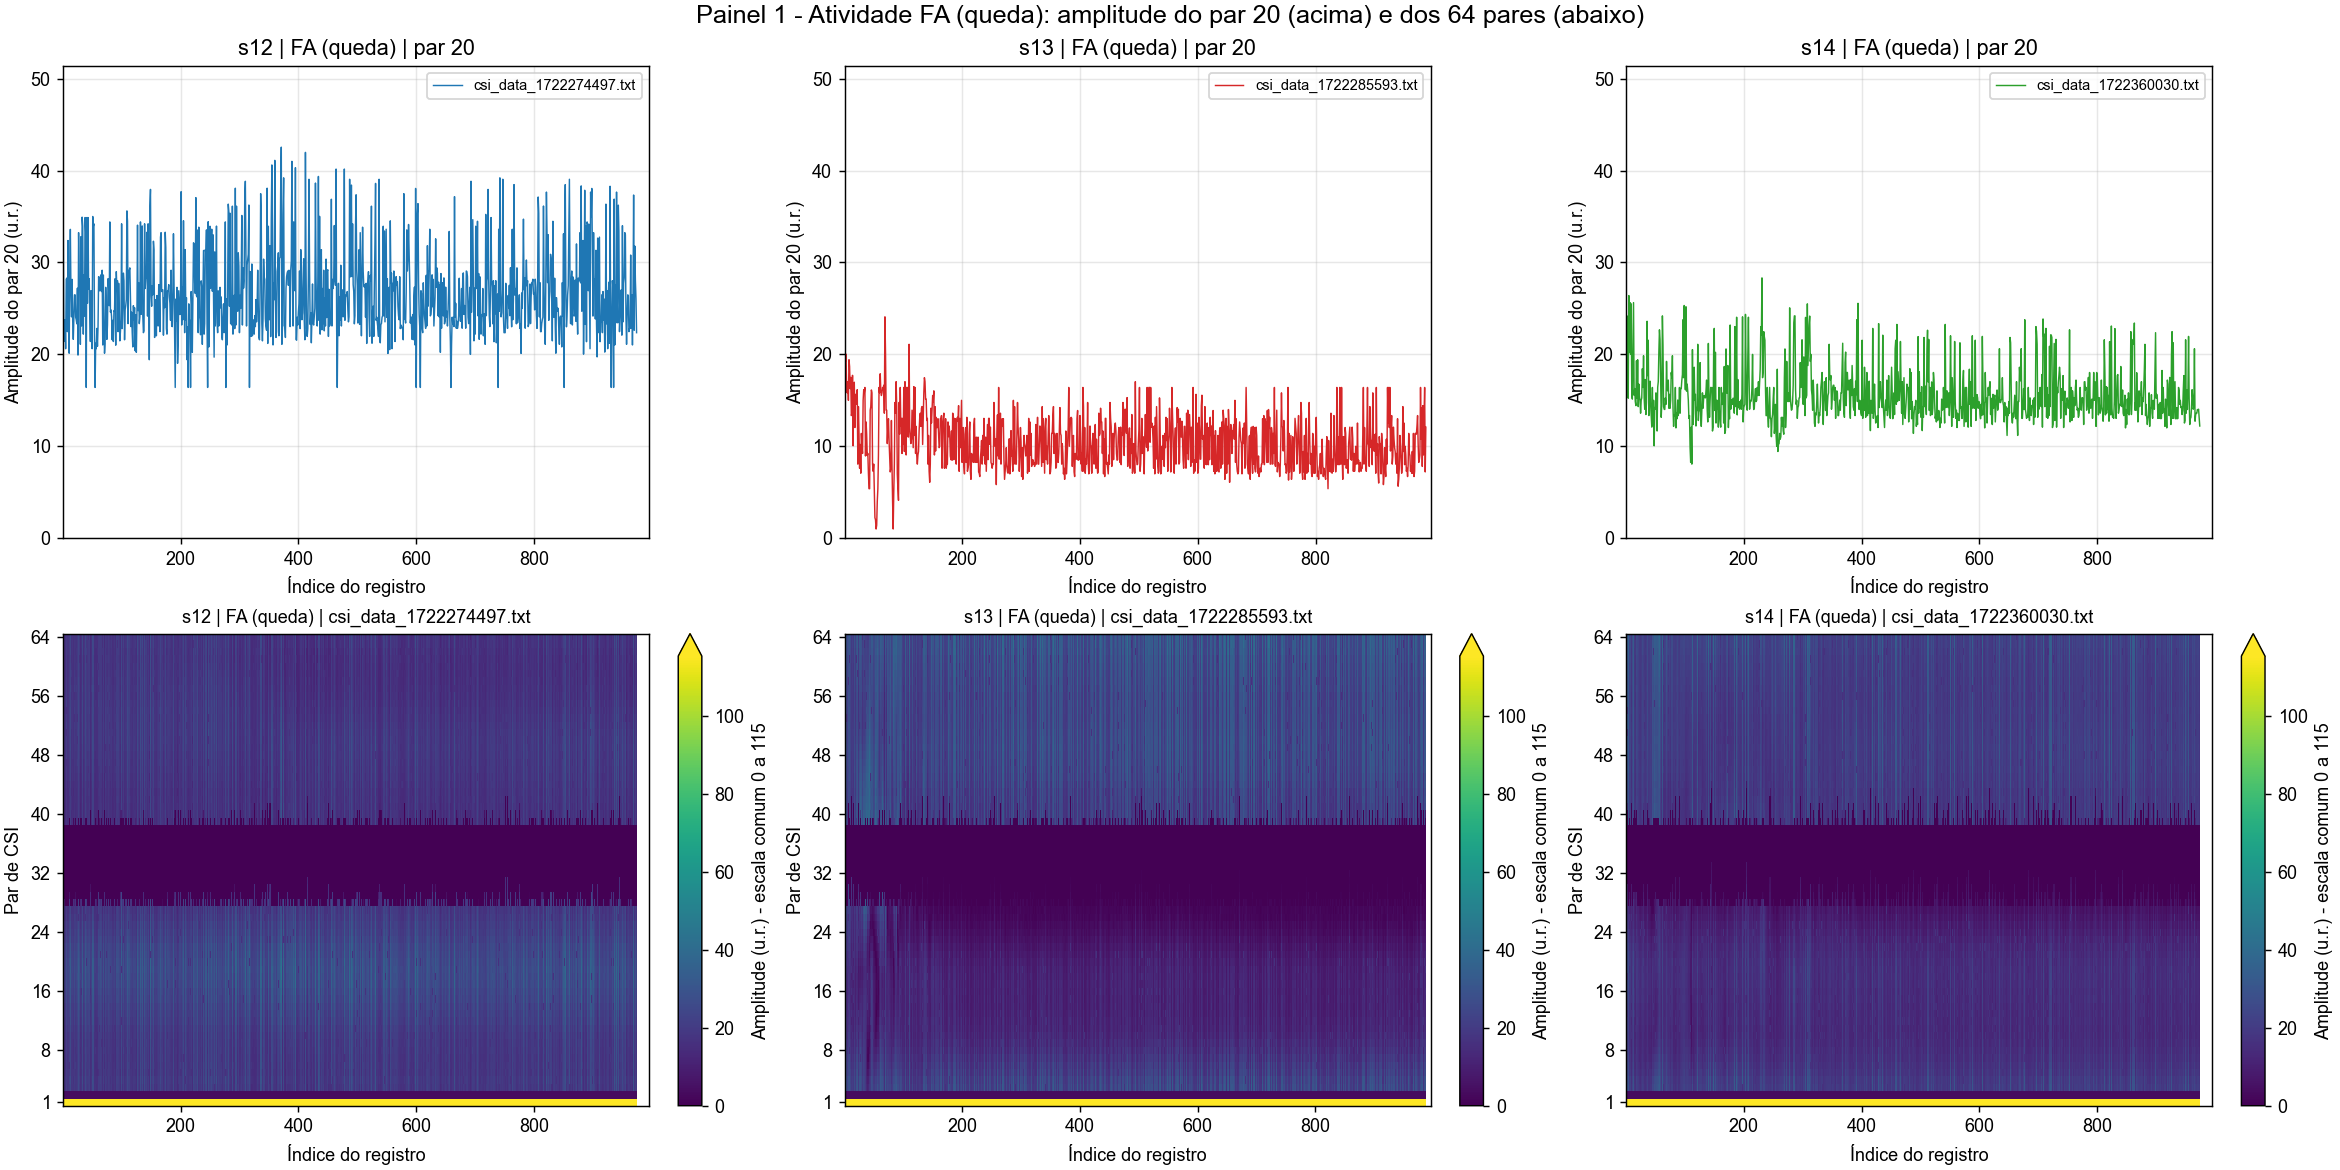
\includegraphics[width=1.00\textwidth,height=19.0cm,keepaspectratio]{Imagens/sec3_painel1_FA.png}
    \caption{Painel 1 - atividade FA (queda): séries temporais do par 20 (acima) e mapas de calor dos 64 pares (abaixo) para s12, s13 e s14 (ordem\_selecao = 1). (arquivo: figuras/sec3\_painel1\_FA.png)}
    \label{fig:sec3_painel1_FA}
\end{figure}

\begin{figure}[H]
    \centering
    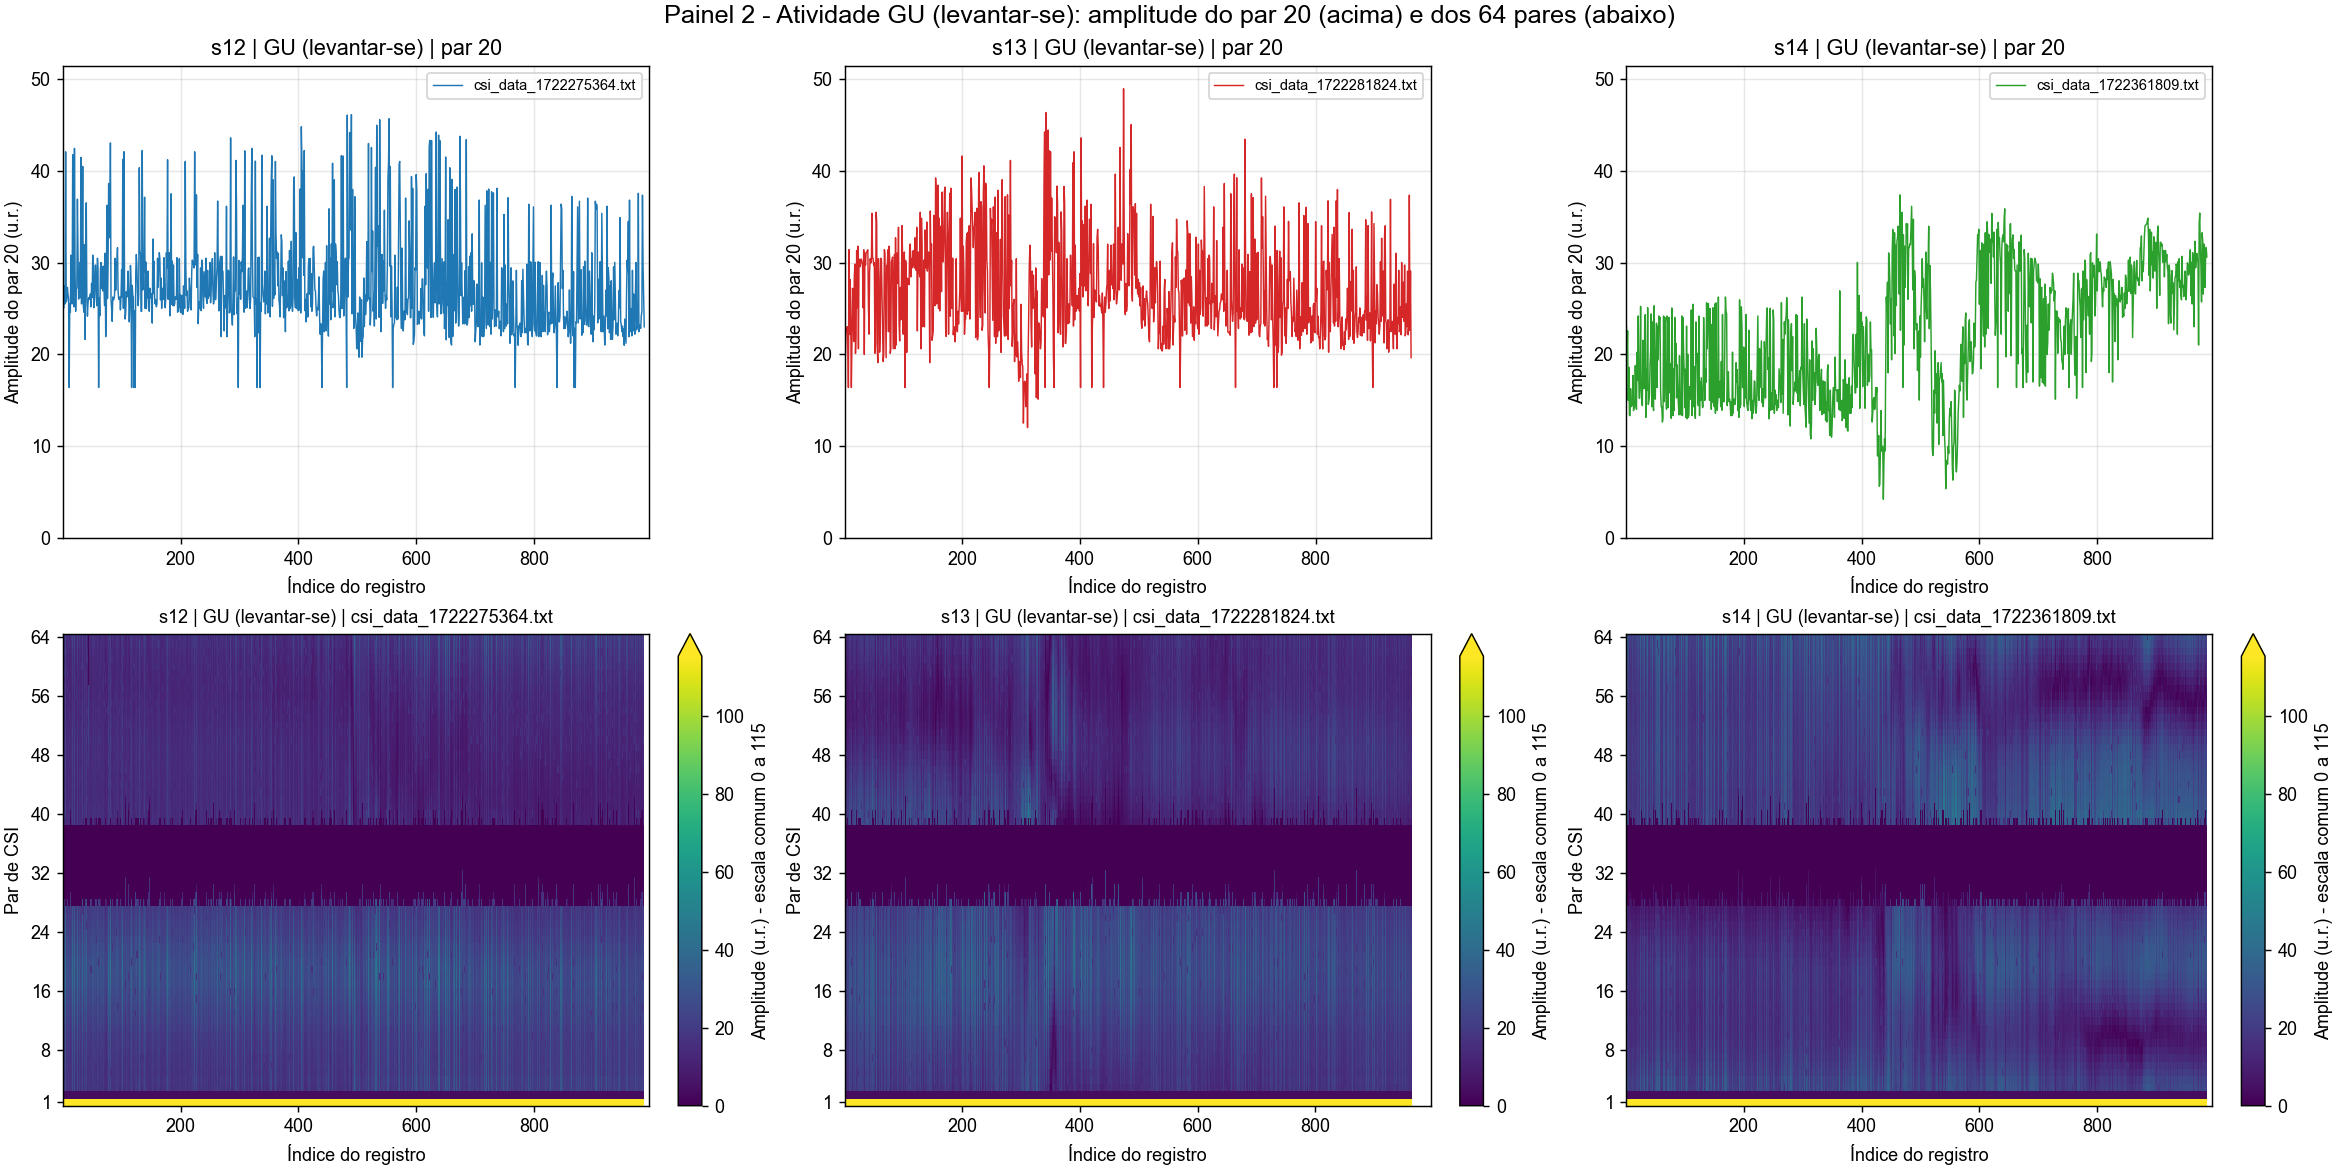
\includegraphics[width=1.00\textwidth,height=19.0cm,keepaspectratio]{Imagens/sec3_painel2_GU.png}
    \caption{Painel 2 - atividade GU (levantar-se): séries temporais do par 20 (acima) e mapas de calor dos 64 pares (abaixo) para s12, s13 e s14 (ordem\_selecao = 1). (arquivo: figuras/sec3\_painel2\_GU.png)}
    \label{fig:sec3_painel2_GU}
\end{figure}

\begin{figure}[H]
    \centering
    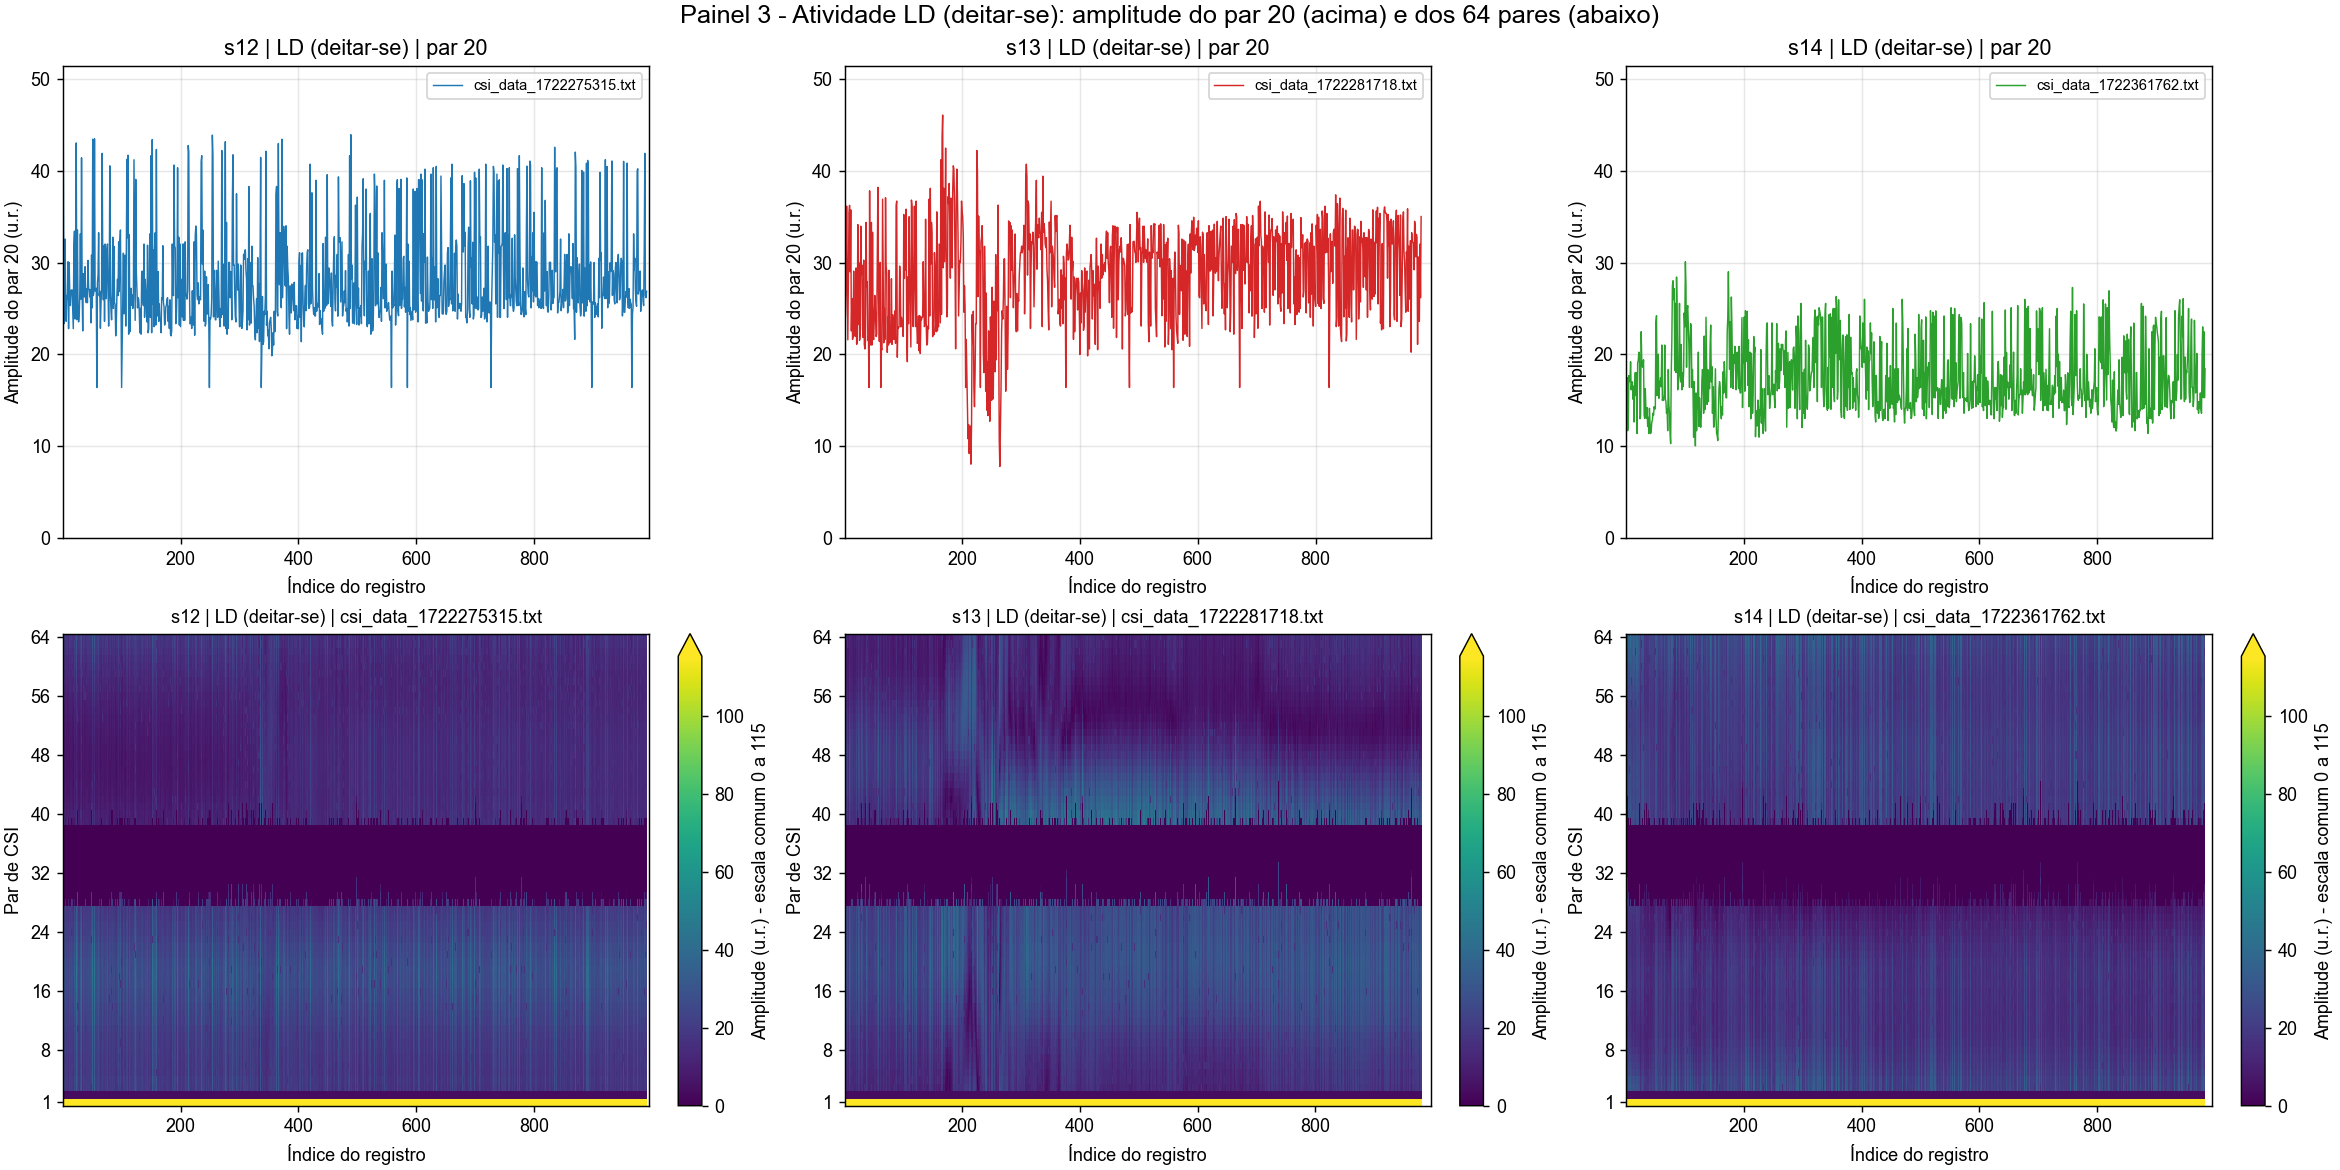
\includegraphics[width=1.00\textwidth,height=19.0cm,keepaspectratio]{Imagens/sec3_painel3_LD.png}
    \caption{Painel 3 - atividade LD (deitar-se): séries temporais do par 20 (acima) e mapas de calor dos 64 pares (abaixo) para s12, s13 e s14 (ordem\_selecao = 1). (arquivo: figuras/sec3\_painel3\_LD.png)}
    \label{fig:sec3_painel3_LD}
\end{figure}

\begin{figure}[H]
    \centering
    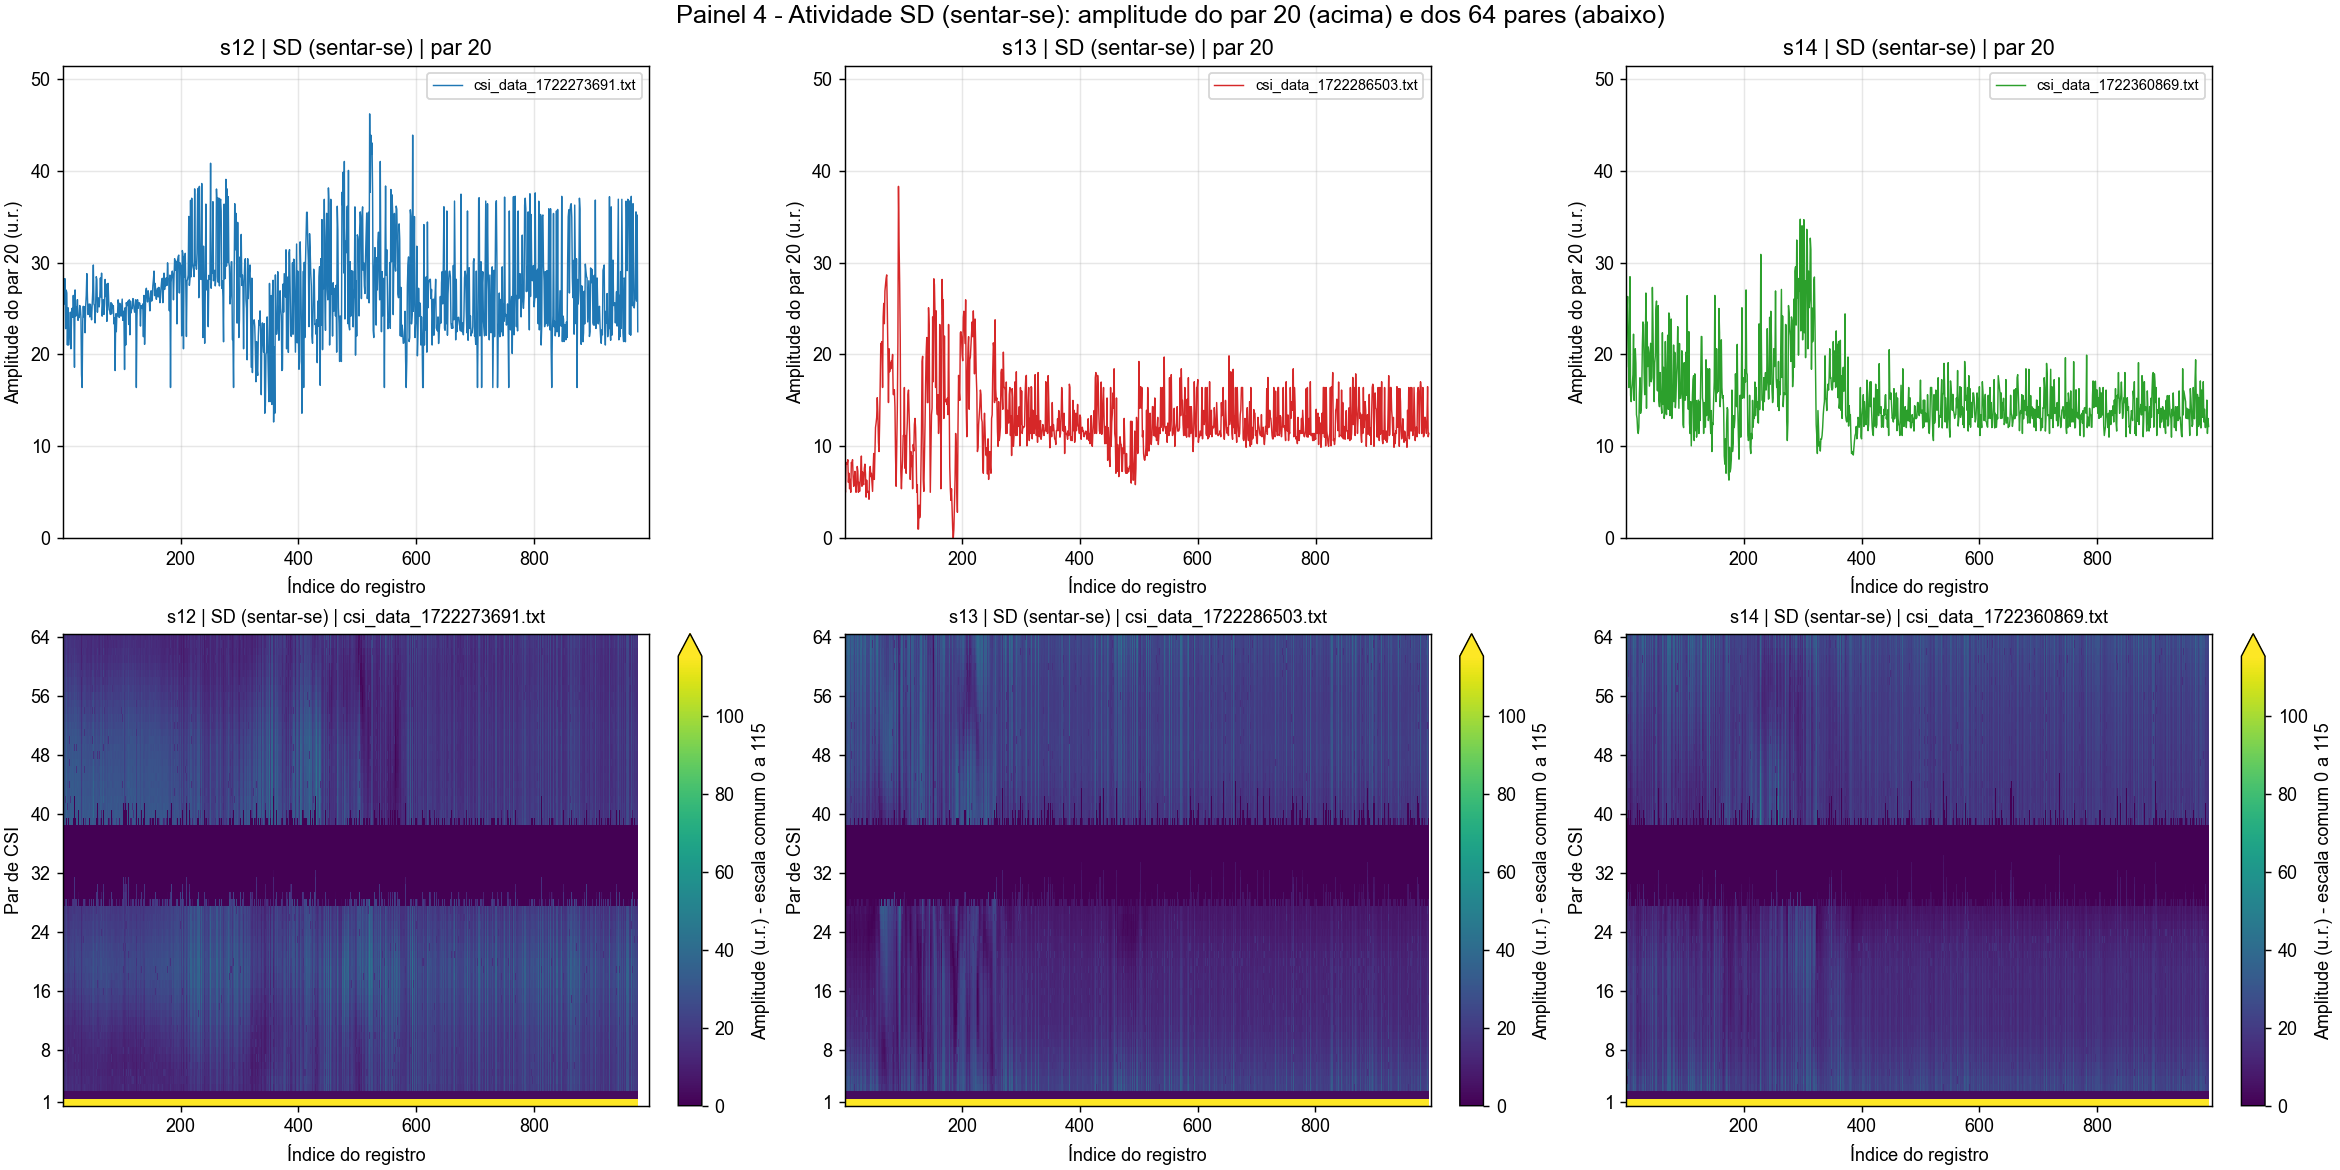
\includegraphics[width=1.00\textwidth,height=19.0cm,keepaspectratio]{Imagens/sec3_painel4_SD.png}
    \caption{Painel 4 - atividade SD (sentar-se): séries temporais do par 20 (acima) e mapas de calor dos 64 pares (abaixo) para s12, s13 e s14 (ordem\_selecao = 1). (arquivo: figuras/sec3\_painel4\_SD.png)}
    \label{fig:sec3_painel4_SD}
\end{figure}

\begin{figure}[H]
    \centering
    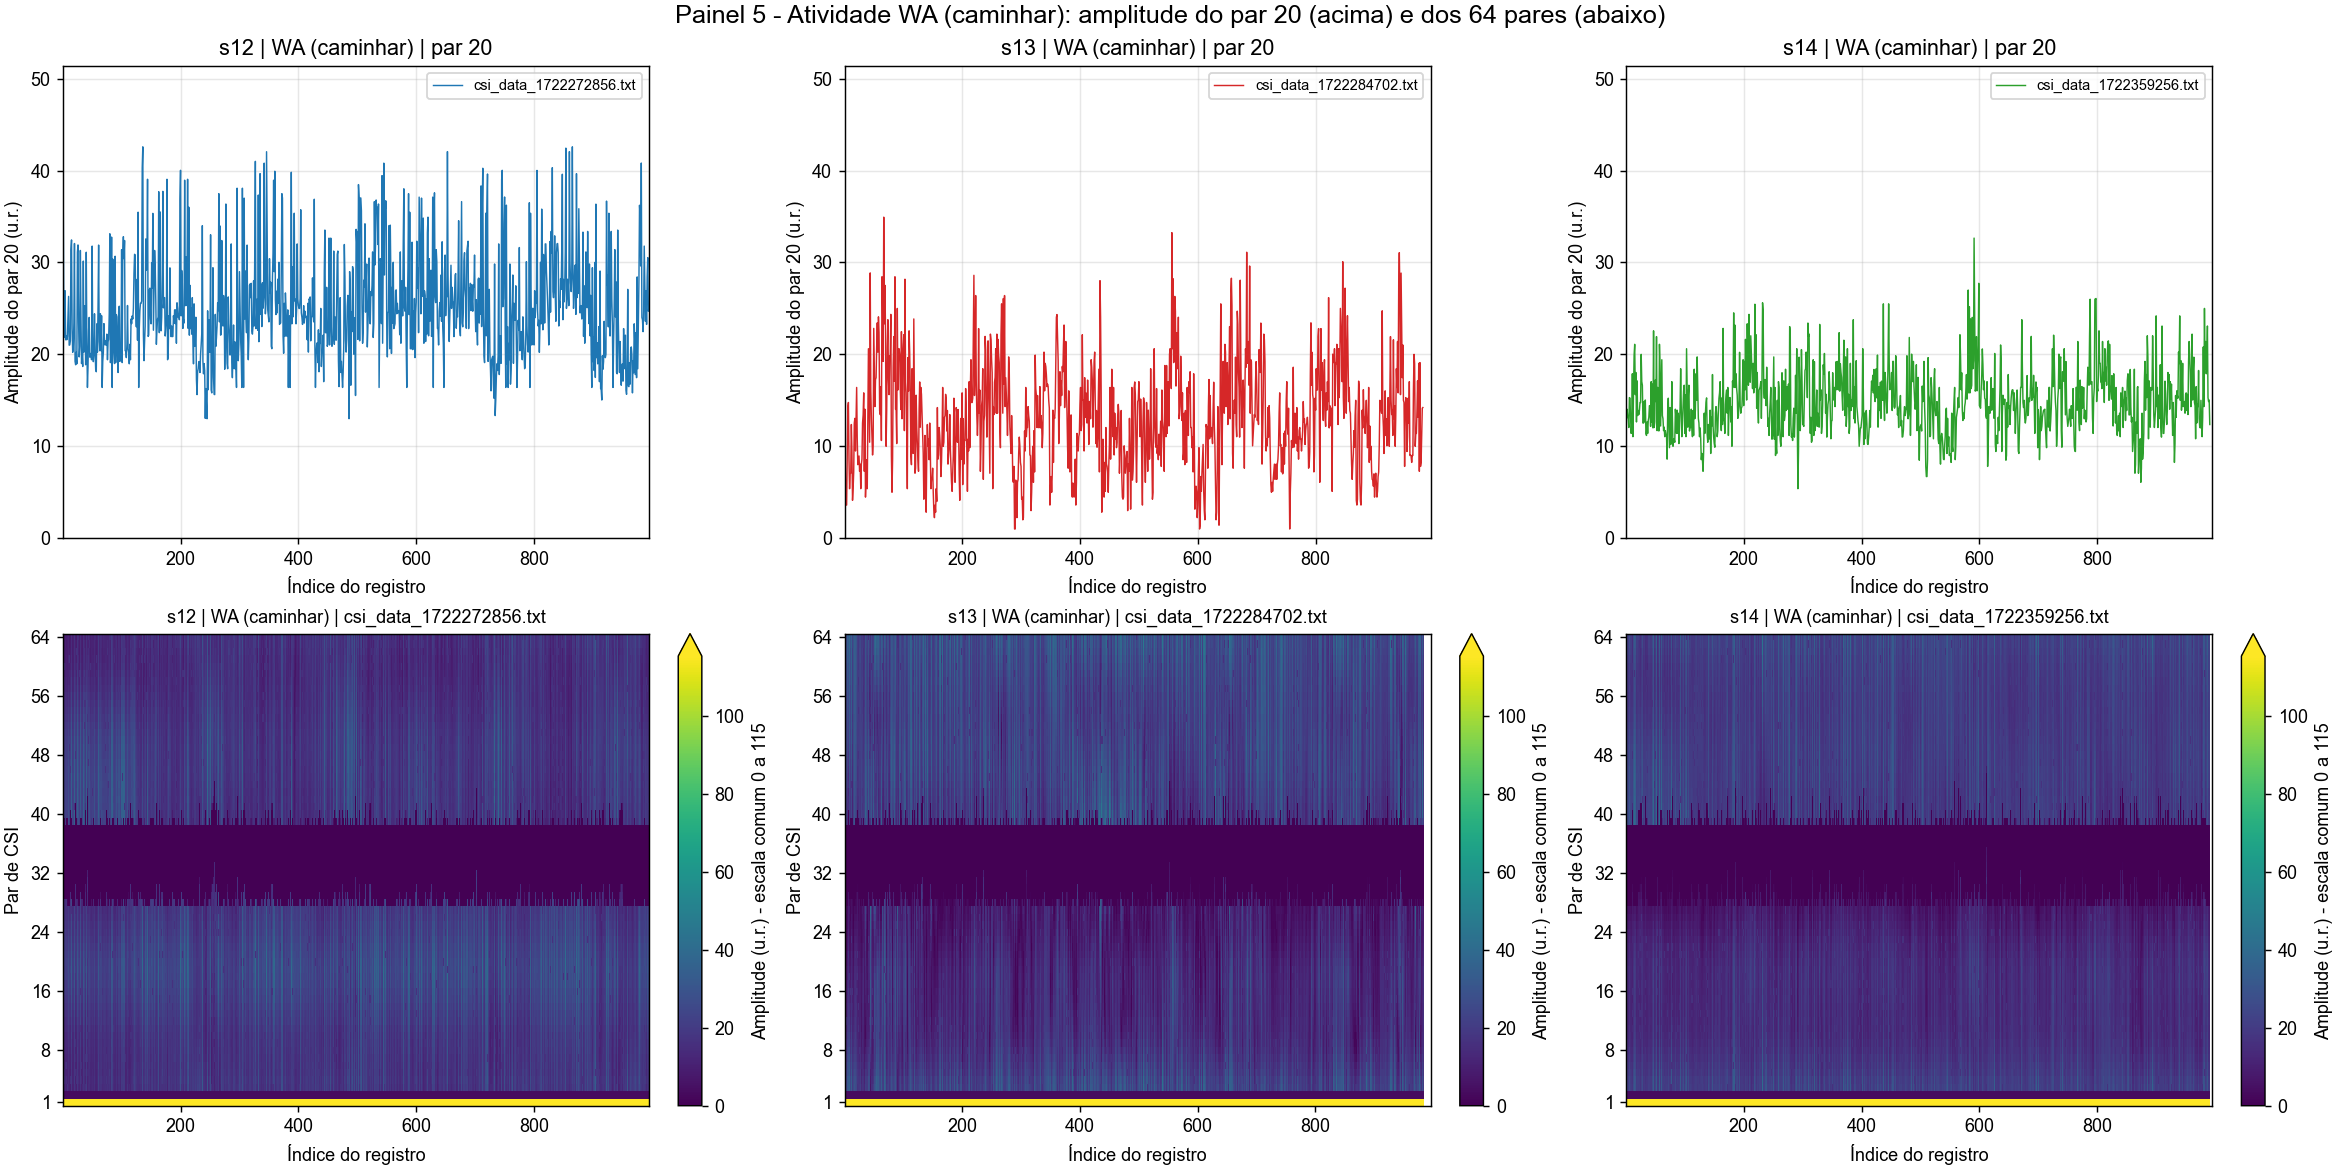
\includegraphics[width=1.00\textwidth,height=19.0cm,keepaspectratio]{Imagens/sec3_painel5_WA.png}
    \caption{Painel 5 - atividade WA (caminhar): séries temporais do par 20 (acima) e mapas de calor dos 64 pares (abaixo) para s12, s13 e s14 (ordem\_selecao = 1). (arquivo: figuras/sec3\_painel5\_WA.png)}
    \label{fig:sec3_painel5_WA}
\end{figure}

\subsection{Interpretação}

\textbf{1. Mesma atividade, pessoas diferentes.} A característica mais evidente é o \textbf{nível} da amplitude do par 20, que difere mais entre participantes do que entre atividades: s12 oscila em torno de 25-28 em todas as atividades, s14 em torno de 15-22, e s13 tem dois níveis (cerca de 10-13 em FA, SD e WA e cerca de 27-29 em GU e LD). Quanto à forma:

\begin{itemize}
    \item \textbf{SD (Figura 4)} é a atividade com maior semelhança entre os três: todos apresentam um trecho inicial perturbado seguido de um trecho estável. Em s13 a perturbação ocupa os registros $\sim$1-250 (desvio padrão por janela de 100 registros de 7,6, 7,1 e 4,7, caindo para $\sim$2 depois do registro 300); em s14, os registros $\sim$1-400 (pico de $\sim$35 perto do registro 300; depois do registro 400 o desvio por janela fica entre 1,7 e 2,0); em s12 a perturbação é mais tardia, registros $\sim$200-600 (queda até $\sim$13 perto do registro 350 e pico de 46 perto do 520).
    \item \textbf{FA (Figura 1)}: s13 e s14 têm maior variação nos primeiros registros (s13: janela 1-100 com desvio 4,9 contra $\sim$2,5 no restante; s14: registros 1-300 com 3,2-3,8 contra $\sim$2,7), enquanto s12 oscila de forma densa e uniforme (20 a 42) em toda a gravação.
    \item \textbf{GU (Figura 2)}: s14 apresenta grandes mudanças de nível - de $\sim$15-25 até o registro $\sim$400, quedas até $\sim$5 perto dos registros 430 e 550 e subida para $\sim$30 depois do registro 600 (desvio de 8,4 na janela 401-500). s13 varia mais nos registros 201-400 (6,6 e 7,6) e s12 é mais uniforme.
    \item \textbf{LD (Figura 3)}: s13 tem uma perturbação marcada nos registros $\sim$150-300 (quedas até $\sim$8 perto dos registros 210 e 260), visível também no mapa de calor como mudança de cor nos pares 40-64 a partir do registro $\sim$350. s12 e s14 são mais uniformes.
    \item \textbf{WA (Figura 5)}: a variação se distribui ao longo de toda a gravação, sem um único trecho dominante. Em s13 aparecem surtos quase periódicos a cada $\sim$100-150 registros, compatíveis com idas e vindas entre os pontos de caminhada, mas sem anotação não é possível confirmar.
\end{itemize}
\textbf{2. Mesma pessoa, atividades diferentes.} Para \textbf{s13}, FA e SD mostram um transiente no início seguido de sinal estável, WA mostra variação durante toda a gravação, e GU/LD têm nível bem mais alto. Para \textbf{s14}, GU tem as maiores mudanças de nível, SD tem o trecho final mais estável de todas as gravações e FA/LD/WA têm variação moderada e contínua. Para \textbf{s12}, as cinco atividades são visualmente parecidas (mesmo nível, oscilação densa entre $\sim$16 e $\sim$45); apenas SD mostra um trecho claramente diferente (registros $\sim$200-600). Em s12 aparece repetidamente o mesmo valor mínimo de 16,4, consequência de os componentes do CSI serem inteiros (as amplitudes assumem valores discretos).

\textbf{3. Variação durante a gravação.} Os trechos de maior variação (desvio por janela de 100 registros, arquivo apoio\_variacao\_janelas\_par20.csv) são: s13/SD registros 1-200 (7,6 e 7,1), s14/GU 401-600 (8,4 e 7,1), s13/GU 301-400 (7,6), s13/LD 201-300 (7,6) e s12/SD 501-600 (6,3). Os de menor variação são os trechos finais de s14/SD (registros 401-989, 1,7-2,0), s13/SD (301-992, 2,0-2,4) e o trecho inicial de s12/SD (1-200, 2,2-2,6), indicando a pessoa parada. Nas atividades de transição (SD, GU, LD, FA) a variação tende a se concentrar em um trecho; em WA ela é distribuída. O instante exato de cada movimento (por exemplo, da queda) não é afirmado, pois a base não tem anotação temporal.

\textbf{4. Comportamento dos pares.} Nos 15 mapas de calor aparecem sempre as mesmas faixas (estatísticas por par em apoio\_estatisticas\_por\_par.csv):

\begin{itemize}
    \item \textbf{Par 1}: amplitude constante de $\sim$115 (desvio médio 0,05) em todas as gravações - faixa amarela na base dos mapas. Por não variar, não carrega informação sobre o movimento.
    \item \textbf{Par 2}: constante em 4,0 (desvio 0).
    \item \textbf{Pares 33 a 38}: amplitude zero (desvio $\leq$ 0,1) - faixa escura central.
    \item \textbf{Pares 28 a 32}: amplitudes decrescentes e próximas de zero (médias 5,2; 1,6; 0,6; 0,2; 0,06).
    \item \textbf{Par 39}: transição, com média 13,7 mas o maior desvio padrão (10,1).
    \item Os pares 3-27 e 40-64 têm amplitudes de $\sim$15-21 e variação de $\sim$4-5. Isso é coerente com a estrutura do canal 802.11n de 20 MHz descrita no artigo (52 subportadoras de dados, 4 piloto e 8 nulas); os autores removem os índices 0 e 27-37 (pares 1 e 28-38) em imf\_generator.py, ficando com 52 pares.
\end{itemize}
\newpage

\section{Características das amplitudes (seção 4)}

\subsection{Características calculadas}

Para cada uma das 30 gravações foi usada a série completa de amplitudes do par 20, na ordem original e sem normalização, suavização ou corte. As cinco características são:

{\footnotesize
\begin{longtable}{|>{\centering\arraybackslash}p{2.84cm}|>{\centering\arraybackslash}p{4.57cm}|>{\centering\arraybackslash}p{7.24cm}|}
\caption{Características usadas na análise.}\\
\hline
\textbf{Característica} & \textbf{Cálculo} & \textbf{O que mede / para que serve} \\ \hline
\endfirsthead
\hline
\textbf{Característica} & \textbf{Cálculo} & \textbf{O que mede / para que serve} \\ \hline
\endhead
Média & soma das amplitudes / N & Nível médio do sinal. Depende da posição da pessoa, do ambiente e do ganho do receptor; serve para comparar o nível entre gravações. \\ \hline
Mediana & valor central da série ordenada & Nível típico, pouco sensível a picos isolados. Comparada com a média, indica assimetria e presença de valores extremos. \\ \hline
Desvio padrão & raiz da média dos quadrados dos desvios em relação à média, divisor N (ddof = 0) & Dispersão em torno da média: quanto o sinal varia ao longo da gravação (movimento gera variação). \\ \hline
Pico a pico & máximo - mínimo & Extensão total dos valores; muito sensível a um único valor extremo. \\ \hline
Média das diferenças absolutas & soma de |x(i+1) - x(i)| / (N - 1) & Variação média de um registro para o seguinte (rapidez das mudanças por registro, não por segundo). \\ \hline
\end{longtable}
}

Os resultados das 30 gravações estão em \textbf{caracteristicas\_reais.csv} e na Tabela A1 (Anexo).

\subsection{Gráficos comparativos}

Em cada gráfico, o eixo horizontal tem as cinco atividades, cada cor é um participante (azul s12, vermelho s13, verde s14, iguais nos cinco gráficos) e o símbolo distingue a primeira (círculo) e a segunda (triângulo) gravação: 6 pontos por atividade e 30 por gráfico.

\begin{figure}[H]
    \centering
    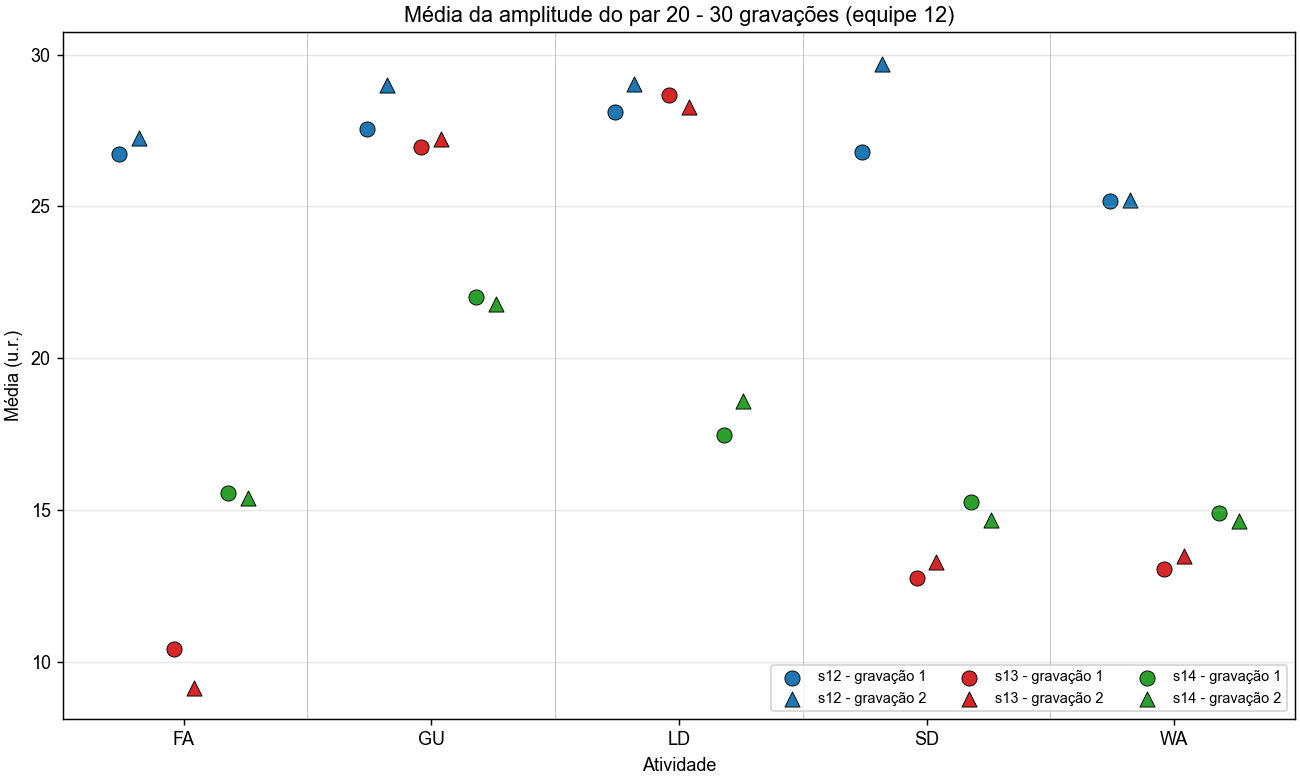
\includegraphics[width=0.85\textwidth,height=19.0cm,keepaspectratio]{Imagens/sec4_grafico1_media.png}
    \caption{Média da amplitude do par 20 nas 30 gravações. (arquivo: figuras/sec4\_grafico1\_media.png)}
    \label{fig:sec4_grafico1_media}
\end{figure}

\begin{figure}[H]
    \centering
    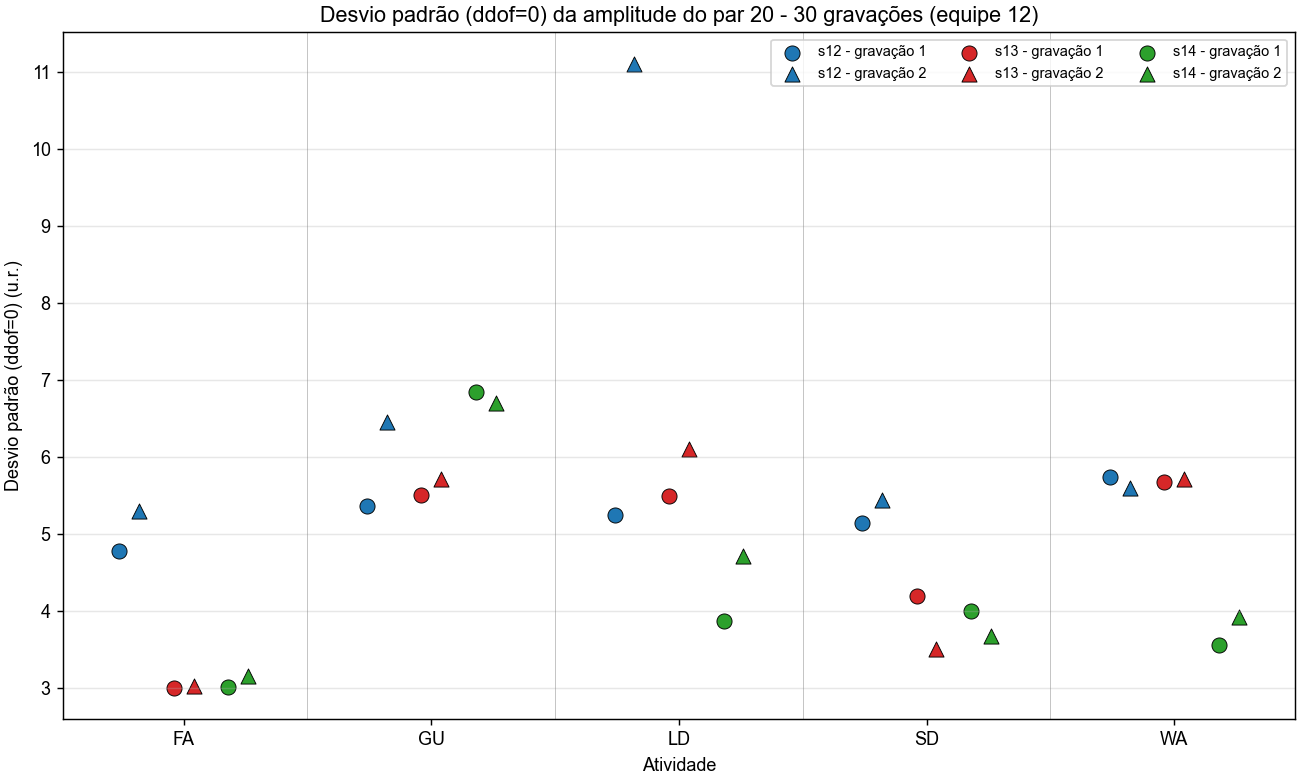
\includegraphics[width=0.85\textwidth,height=19.0cm,keepaspectratio]{Imagens/sec4_grafico3_desvio_padrao.png}
    \caption{Desvio padrão da amplitude do par 20 nas 30 gravações. (arquivo: figuras/sec4\_grafico3\_desvio\_padrao.png)}
    \label{fig:sec4_grafico3_desvio_padrao}
\end{figure}

\begin{figure}[H]
    \centering
    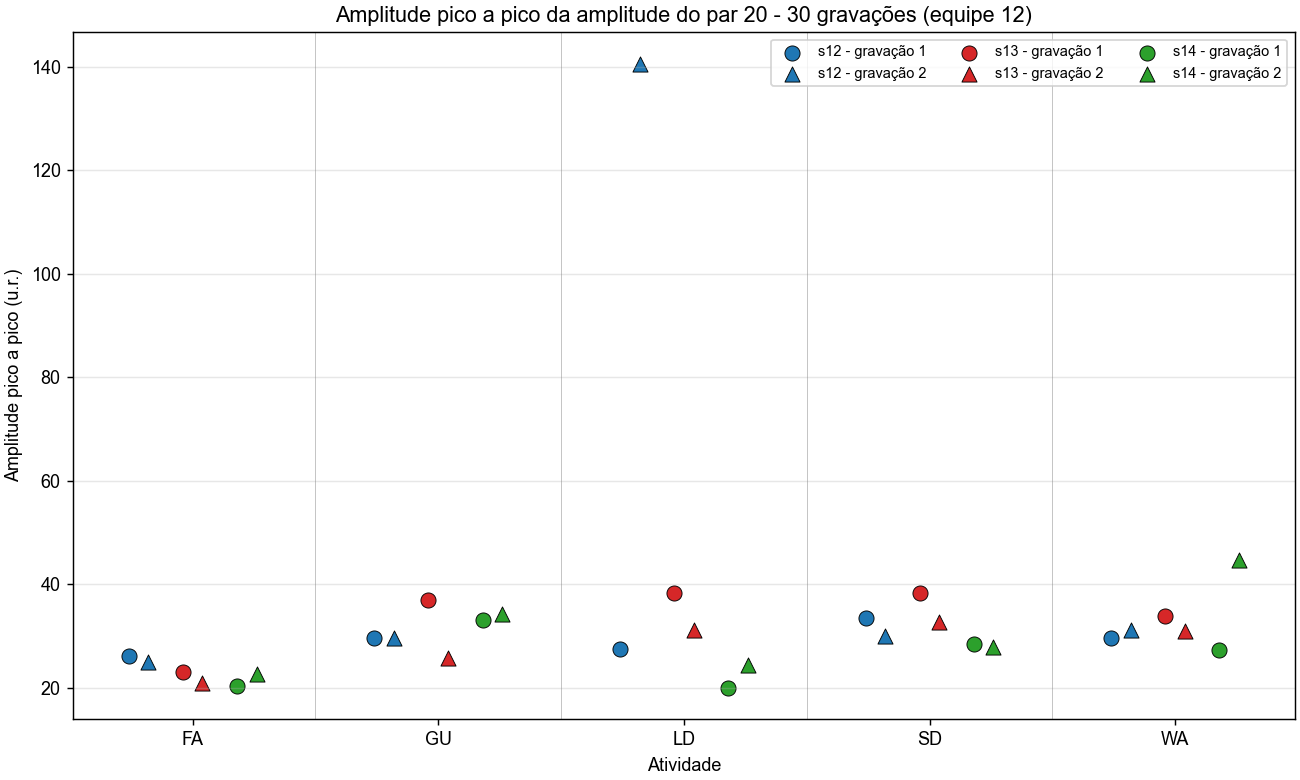
\includegraphics[width=0.85\textwidth,height=19.0cm,keepaspectratio]{Imagens/sec4_grafico4_pico_a_pico.png}
    \caption{Amplitude pico a pico da amplitude do par 20 nas 30 gravações. (arquivo: figuras/sec4\_grafico4\_pico\_a\_pico.png)}
    \label{fig:sec4_grafico4_pico_a_pico}
\end{figure}

\begin{figure}[H]
    \centering
    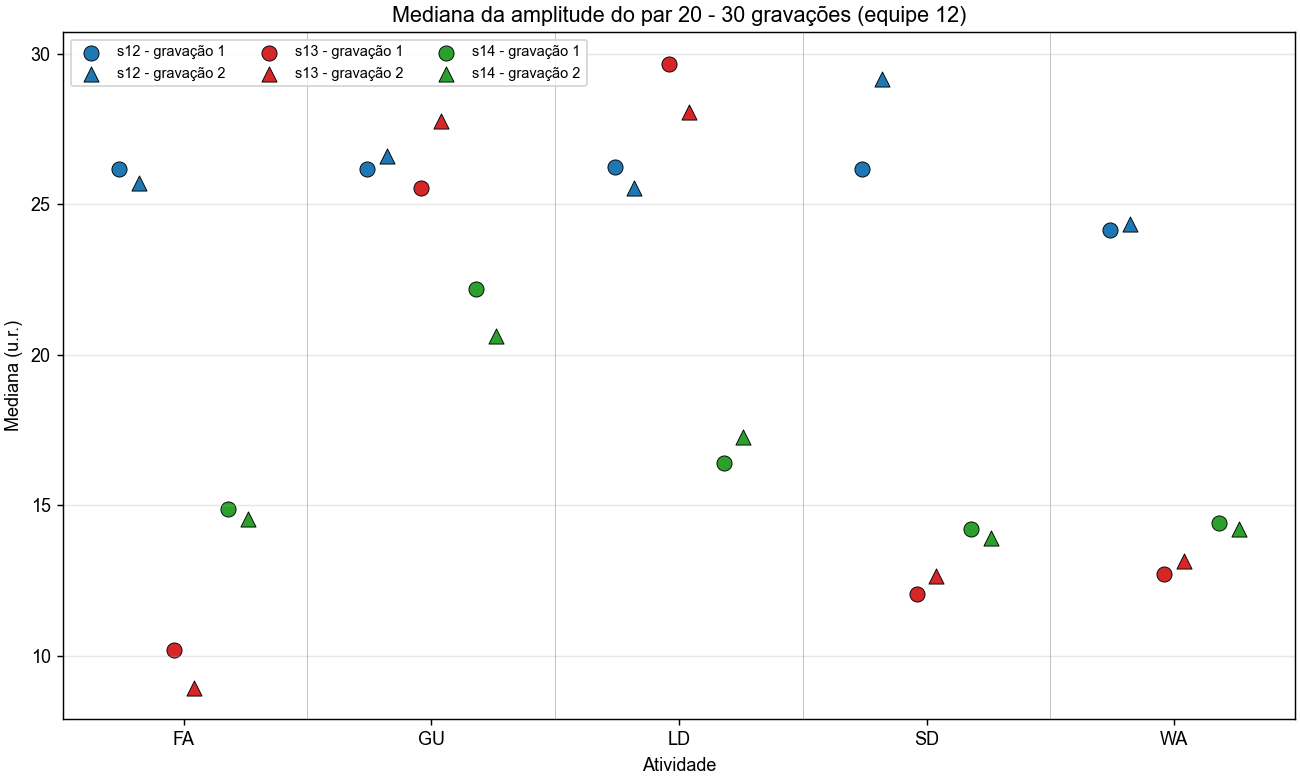
\includegraphics[width=0.85\textwidth,height=19.0cm,keepaspectratio]{Imagens/sec4_grafico2_mediana.png}
    \caption{Mediana da amplitude do par 20 nas 30 gravações. (arquivo: figuras/sec4\_grafico2\_mediana.png)}
    \label{fig:sec4_grafico2_mediana}
\end{figure}

\begin{figure}[H]
    \centering
    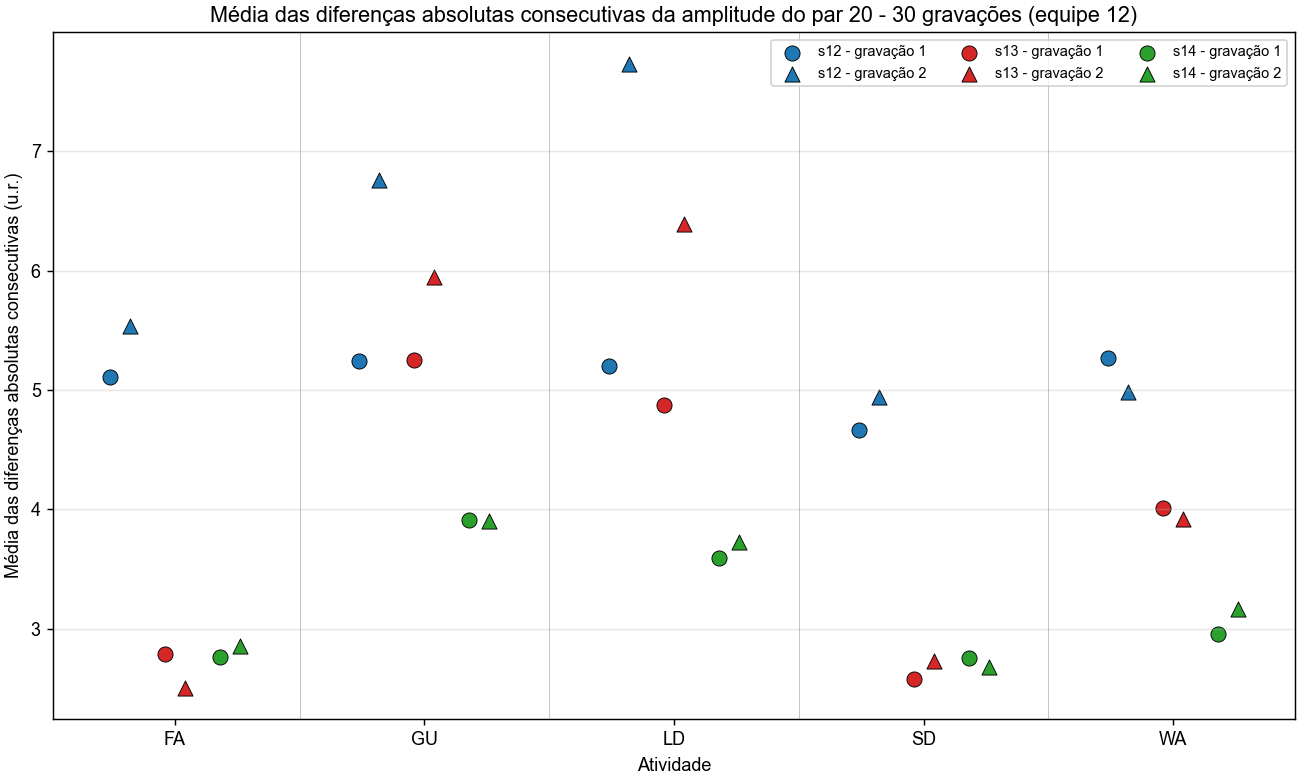
\includegraphics[width=0.85\textwidth,height=19.0cm,keepaspectratio]{Imagens/sec4_grafico5_media_diferencas_absolutas.png}
    \caption{Média das diferenças absolutas entre registros consecutivos da amplitude do par 20 nas 30 gravações. (arquivo: figuras/sec4\_grafico5\_media\_diferencas\_absolutas.png)}
    \label{fig:sec4_grafico5_media_diferencas_absolutas}
\end{figure}

\subsection{Interpretação}

\textbf{1. Duas gravações da mesma pessoa e atividade.} Na maioria dos casos as duas gravações têm características semelhantes. Exemplos: s14/FA, média 15,59 e 15,42, desvio 3,01 e 3,17; s13/WA, média 13,08 e 13,52, desvio 5,68 e 5,71 (Figuras 6 e 7). As exceções são: \textbf{s12/LD}, em que a gravação 2 tem desvio 11,11 contra 5,25, pico a pico 140,63 contra 27,51 e diferença média 7,74 contra 5,20, por causa de picos de até 157 nos registros $\sim$1-250 (visíveis na figura de comparação da dupla s12\_LD, seção 6), enquanto as médias ficam próximas (28,11 e 29,04); \textbf{s12/SD}, com médias 26,80 e 29,70; e \textbf{s14/WA}, com pico a pico 27,26 e 44,69 apesar de desvios parecidos (3,56 e 3,92) - ou seja, um único valor extremo altera o pico a pico sem mudar a dispersão geral.

\textbf{2. Pessoas diferentes, mesma atividade.} Há diferenças acentuadas entre participantes, principalmente no nível (Figuras 6 e 9). Em FA, as médias são 26,72-27,25 (s12), 9,18-10,45 (s13) e 15,42-15,59 (s14), sem sobreposição. Em GU e LD, s12 e s13 se sobrepõem (médias entre $\sim$27 e $\sim$29), enquanto s14 fica abaixo ($\sim$22 em GU e $\sim$17,5-18,6 em LD). A média das diferenças absolutas (Figura 10) também separa os participantes: s12 fica entre 4,7 e 7,7, enquanto s14 fica entre 2,7 e 3,9 em todas as atividades.

\textbf{3. Mesma pessoa, atividades diferentes.} Em \textbf{s13} a média é a característica que mais muda (de 9,18 em FA a 28,67 em LD), acompanhada da diferença média (2,51-2,79 em FA e 2,58-2,73 em SD contra 5,25-5,94 em GU e 4,87-6,39 em LD). Em \textbf{s14}, GU se destaca pelo desvio padrão (6,70-6,84 contra 3,01-3,17 em FA) e pela média ($\sim$22 contra 14,7-18,6 nas demais). Em \textbf{s12} as cinco características variam pouco entre atividades (médias de 25,2 a 29,7; desvios de 4,8 a 6,4, exceto a gravação 2 de LD). Uma hipótese para o caso de s13: os nomes dos arquivos são carimbos de tempo Unix, e as gravações de GU e LD (1722281718 a 1722281947) foram feitas cerca de uma hora antes das de FA, SD e WA (1722284702 a 1722286550). A diferença de nível pode, portanto, refletir mudanças do ambiente ou da posição dos equipamentos entre sessões, e não apenas a atividade.

\textbf{4. Sobreposição entre atividades.} Sim, os valores se sobrepõem bastante. Considerando os três participantes juntos, as médias de FA vão de 9,2 a 27,2 e as de SD de 12,8 a 29,7, cobrindo praticamente a mesma faixa; o pico a pico fica entre $\sim$20 e $\sim$45 em todas as atividades (exceto o valor atípico de s12/LD); e o desvio padrão fica entre $\sim$3 e $\sim$7 para todas. Como a diferença entre pessoas é maior que a diferença entre atividades, essas cinco características de um único par não bastam para distinguir as atividades. Essas conclusões se limitam às 30 gravações analisadas, e a separação visual de pontos não demonstra, por si só, que um classificador reconheceria as atividades.

\newpage

\section{Sinais sintéticos por EEMD (seção 5)}

\subsection{Conceitos}

\textbf{EMD} (\textit{Empirical Mode Decomposition}) decompõe um sinal em componentes oscilatórias de forma adaptativa, sem bases pré-definidas. O processo de peneiramento (\textit{sifting}) localiza os máximos e mínimos locais, interpola envoltórias superior e inferior, subtrai a média das envoltórias e repete até obter uma \textbf{IMF} (\textit{Intrinsic Mode Function}): uma componente cujo número de extremos e de cruzamentos por zero difere no máximo em um e cuja média das envoltórias é aproximadamente zero. A IMF é subtraída do sinal e o processo continua; a IMF1 contém as oscilações mais rápidas e as seguintes, oscilações cada vez mais lentas. O que sobra ao final é o \textbf{resíduo}, uma tendência lenta (monotônica ou com poucos extremos) que representa o nível do sinal. A soma de todas as IMFs com o resíduo reconstrói o sinal.

\textbf{EEMD} (\textit{Ensemble EMD}) é uma variante que reduz a mistura de modos (quando oscilações de escalas muito diferentes caem na mesma IMF): a EMD é aplicada muitas vezes ao sinal somado a ruído branco diferente em cada tentativa, e as IMFs de mesmo índice são promediadas. O ruído tende a se cancelar na média, mas não totalmente; por isso a soma das IMFs da EEMD não reconstrói o sinal com exatidão (erro de reconstrução). O artigo descreve o método como EMD, mas o código dos autores usa EEMD.

\textbf{Exemplo com a dupla s12\_FA (Figura 11):} a série A (csi\_data\_1722274497.txt, 963 valores) foi decomposta em 7 IMFs e um resíduo. A IMF1 contém a oscilação rápida de registro para registro (±10); a IMF3 e a IMF4 oscilam com períodos de dezenas de registros; a IMF7 tem apenas cerca de dois ciclos ao longo dos 963 registros; o resíduo é uma curva suave entre 26,1 e 27,9, que corresponde ao nível médio da série (26,72). A série B (csi\_data\_1722274542.txt) tem estrutura semelhante, com resíduo entre 27,1 e 27,6.

\subsection{Código utilizado e adaptações}

{\footnotesize
\begin{longtable}{|>{\centering\arraybackslash}p{1.92cm}|>{\centering\arraybackslash}p{2.76cm}|>{\centering\arraybackslash}p{4.18cm}|>{\centering\arraybackslash}p{5.35cm}|}
\caption{Procedimentos mantidos e adaptados em relação ao código dos autores.}\\
\hline
\textbf{Etapa} & \textbf{Script dos autores} & \textbf{Mantido} & \textbf{Adaptado pela equipe} \\ \hline
\endfirsthead
\hline
\textbf{Etapa} & \textbf{Script dos autores} & \textbf{Mantido} & \textbf{Adaptado pela equipe} \\ \hline
\endhead
Amplitudes & CSI.py (get\_amps) & Ordem imaginária/real e fórmula da amplitude & Cálculo vetorizado; sem substituir NaN por 0 (as séries são todas finitas) \\ \hline
Decomposição & imf\_generator.py & PyEMD EEMD(trials=100), noise\_seed(5), max\_imf=7 (7 IMFs + resíduo, como no artigo) & Apenas o par 20, com N valores (em vez de 52 subportadoras truncadas em 850); separate\_trends=True (ver 6.3); nova instância e mesma semente para cada série; sem salvar arquivos intermediários \\ \hline
Seleção alternada & imf\_sample\_builder.py & IMFs de índice ímpar (IMF1, IMF3, ...) de A e de índice par (IMF2, IMF4, ...) de B & Uma única dupla por participante/atividade (A = ordem 1, B = ordem 2); o resíduo não entra na alternância: usa-se a média dos resíduos de A e B \\ \hline
Soma & dataset\_constructor.py (SYNTHETIC DATASET GENERATION) & Soma das componentes selecionadas & Sem a divisão em treino e teste; vetores salvos em sinais\_sinteticos.npz \\ \hline
\end{longtable}
}

\subsection{Configuração, regra de recombinação e tratamento dos resíduos}

\begin{itemize}
    \item Biblioteca: EMD-signal (PyEMD) 1.10.0, classe EEMD, com trials = 100, noise\_width = 0,05 (padrão: desvio do ruído = 5\% da faixa do sinal), max\_imf = 7, separate\_trends = True e semente aleatória 5 (noise\_seed(5)), reiniciada para cada série, o que torna o processamento repetível.
    \item Como a biblioteca disponibiliza as componentes: eemd() devolve a matriz E\_IMF (média do ensemble). Com separate\_trends = True, a última linha é a tendência (resíduo) de cada tentativa promediada e as anteriores são as IMFs. O atributo residue da biblioteca (sinal - soma de E\_IMF) não é o resíduo da decomposição, mas o erro de reconstrução da EEMD; ele foi descartado, como no código dos autores, e seu desvio padrão foi registrado em duplas\_eemd.csv (entre 0,69 e 1,64, exceto 4,95 na série B de s12\_LD, que contém picos).
    \item \textbf{Por que separate\_trends = True:} na primeira execução, sem essa opção (como no código dos autores), metade das 100 tentativas da série A de s13\_LD produziu só 6 IMFs, e a tendência caiu no índice 6 em vez do 7. A média do ensemble espalhou o nível do sinal entre a IMF7 (média 14,2) e o resíduo, e a recombinação somou esse nível duas vezes: o sinal sintético ficou com média $\sim$43, contra $\sim$28 nas séries reais. Com a opção, a tendência de cada tentativa fica sempre na última posição.
    \item \textbf{Componentes usadas} (iguais nas 15 duplas): IMF1 de A + IMF2 de B + IMF3 de A + IMF4 de B + IMF5 de A + IMF6 de B + IMF7 de A + (resíduo de A + resíduo de B) / 2. A média dos resíduos preserva o nível das duas gravações sem privilegiar nenhuma.
    \item \textbf{Regra para quantidades diferentes de IMFs:} usar os índices comuns 1..k, com k = min(nA, nB), alternando A e B; as IMFs excedentes (as mais lentas) são somadas ao resíduo da própria série antes da média dos resíduos, para não descartar tendência. Nas 30 séries a EEMD produziu 7 IMFs (limite max\_imf), portanto a regra não precisou ser acionada.
\end{itemize}
\subsection{Duplas e ajuste de comprimento}

Cada dupla une a gravação A (ordem\_selecao = 1) e a B (ordem\_selecao = 2) do mesmo participante e atividade. As duas séries do par 20 foram cortadas nos primeiros N valores, N = comprimento da mais curta. Os TXT originais não foram alterados. Esse ajuste iguala os comprimentos, mas não alinha os instantes dos movimentos.

{\footnotesize
\begin{longtable}{|>{\centering\arraybackslash}p{1.07cm}|>{\centering\arraybackslash}p{2.58cm}|>{\centering\arraybackslash}p{2.58cm}|>{\centering\arraybackslash}p{0.93cm}|>{\centering\arraybackslash}p{0.93cm}|>{\centering\arraybackslash}p{0.79cm}|>{\centering\arraybackslash}p{1.00cm}|>{\centering\arraybackslash}p{1.00cm}|>{\centering\arraybackslash}p{1.07cm}|}
\caption{As 15 duplas: arquivos de origem, quantidade original de amplitudes, N utilizado e valores removidos de A e B.}\\
\hline
\textbf{Dupla} & \textbf{Arquivo A} & \textbf{Arquivo B} & \textbf{Orig. A} & \textbf{Orig. B} & \textbf{N} & \textbf{Remov. A} & \textbf{Remov. B} & \textbf{IMFs A/B} \\ \hline
\endfirsthead
\hline
\textbf{Dupla} & \textbf{Arquivo A} & \textbf{Arquivo B} & \textbf{Orig. A} & \textbf{Orig. B} & \textbf{N} & \textbf{Remov. A} & \textbf{Remov. B} & \textbf{IMFs A/B} \\ \hline
\endhead
s12\_FA & csi\_data\_1722274497.txt & csi\_data\_1722274542.txt & 974 & 963 & 963 & 11 & 0 & 7/7 \\ \hline
s12\_GU & csi\_data\_1722275364.txt & csi\_data\_1722275473.txt & 987 & 990 & 987 & 0 & 3 & 7/7 \\ \hline
s12\_LD & csi\_data\_1722275315.txt & csi\_data\_1722275426.txt & 991 & 936 & 936 & 55 & 0 & 7/7 \\ \hline
s12\_SD & csi\_data\_1722273691.txt & csi\_data\_1722273739.txt & 976 & 978 & 976 & 0 & 2 & 7/7 \\ \hline
s12\_WA & csi\_data\_1722272856.txt & csi\_data\_1722272903.txt & 995 & 994 & 994 & 1 & 0 & 7/7 \\ \hline
s13\_FA & csi\_data\_1722285593.txt & csi\_data\_1722285652.txt & 987 & 978 & 978 & 9 & 0 & 7/7 \\ \hline
s13\_GU & csi\_data\_1722281824.txt & csi\_data\_1722281947.txt & 962 & 986 & 962 & 0 & 24 & 7/7 \\ \hline
s13\_LD & csi\_data\_1722281718.txt & csi\_data\_1722281887.txt & 979 & 983 & 979 & 0 & 4 & 7/7 \\ \hline
s13\_SD & csi\_data\_1722286503.txt & csi\_data\_1722286550.txt & 992 & 991 & 991 & 1 & 0 & 7/7 \\ \hline
s13\_WA & csi\_data\_1722284702.txt & csi\_data\_1722284759.txt & 982 & 975 & 975 & 7 & 0 & 7/7 \\ \hline
s14\_FA & csi\_data\_1722360030.txt & csi\_data\_1722360079.txt & 974 & 992 & 974 & 0 & 18 & 7/7 \\ \hline
s14\_GU & csi\_data\_1722361809.txt & csi\_data\_1722361907.txt & 986 & 994 & 986 & 0 & 8 & 7/7 \\ \hline
s14\_LD & csi\_data\_1722361762.txt & csi\_data\_1722361861.txt & 983 & 990 & 983 & 0 & 7 & 7/7 \\ \hline
s14\_SD & csi\_data\_1722360869.txt & csi\_data\_1722360914.txt & 989 & 977 & 977 & 12 & 0 & 7/7 \\ \hline
s14\_WA & csi\_data\_1722359256.txt & csi\_data\_1722359307.txt & 991 & 980 & 980 & 11 & 0 & 7/7 \\ \hline
\end{longtable}
}

\subsection{Exemplo completo de decomposição}

\begin{figure}[H]
    \centering
    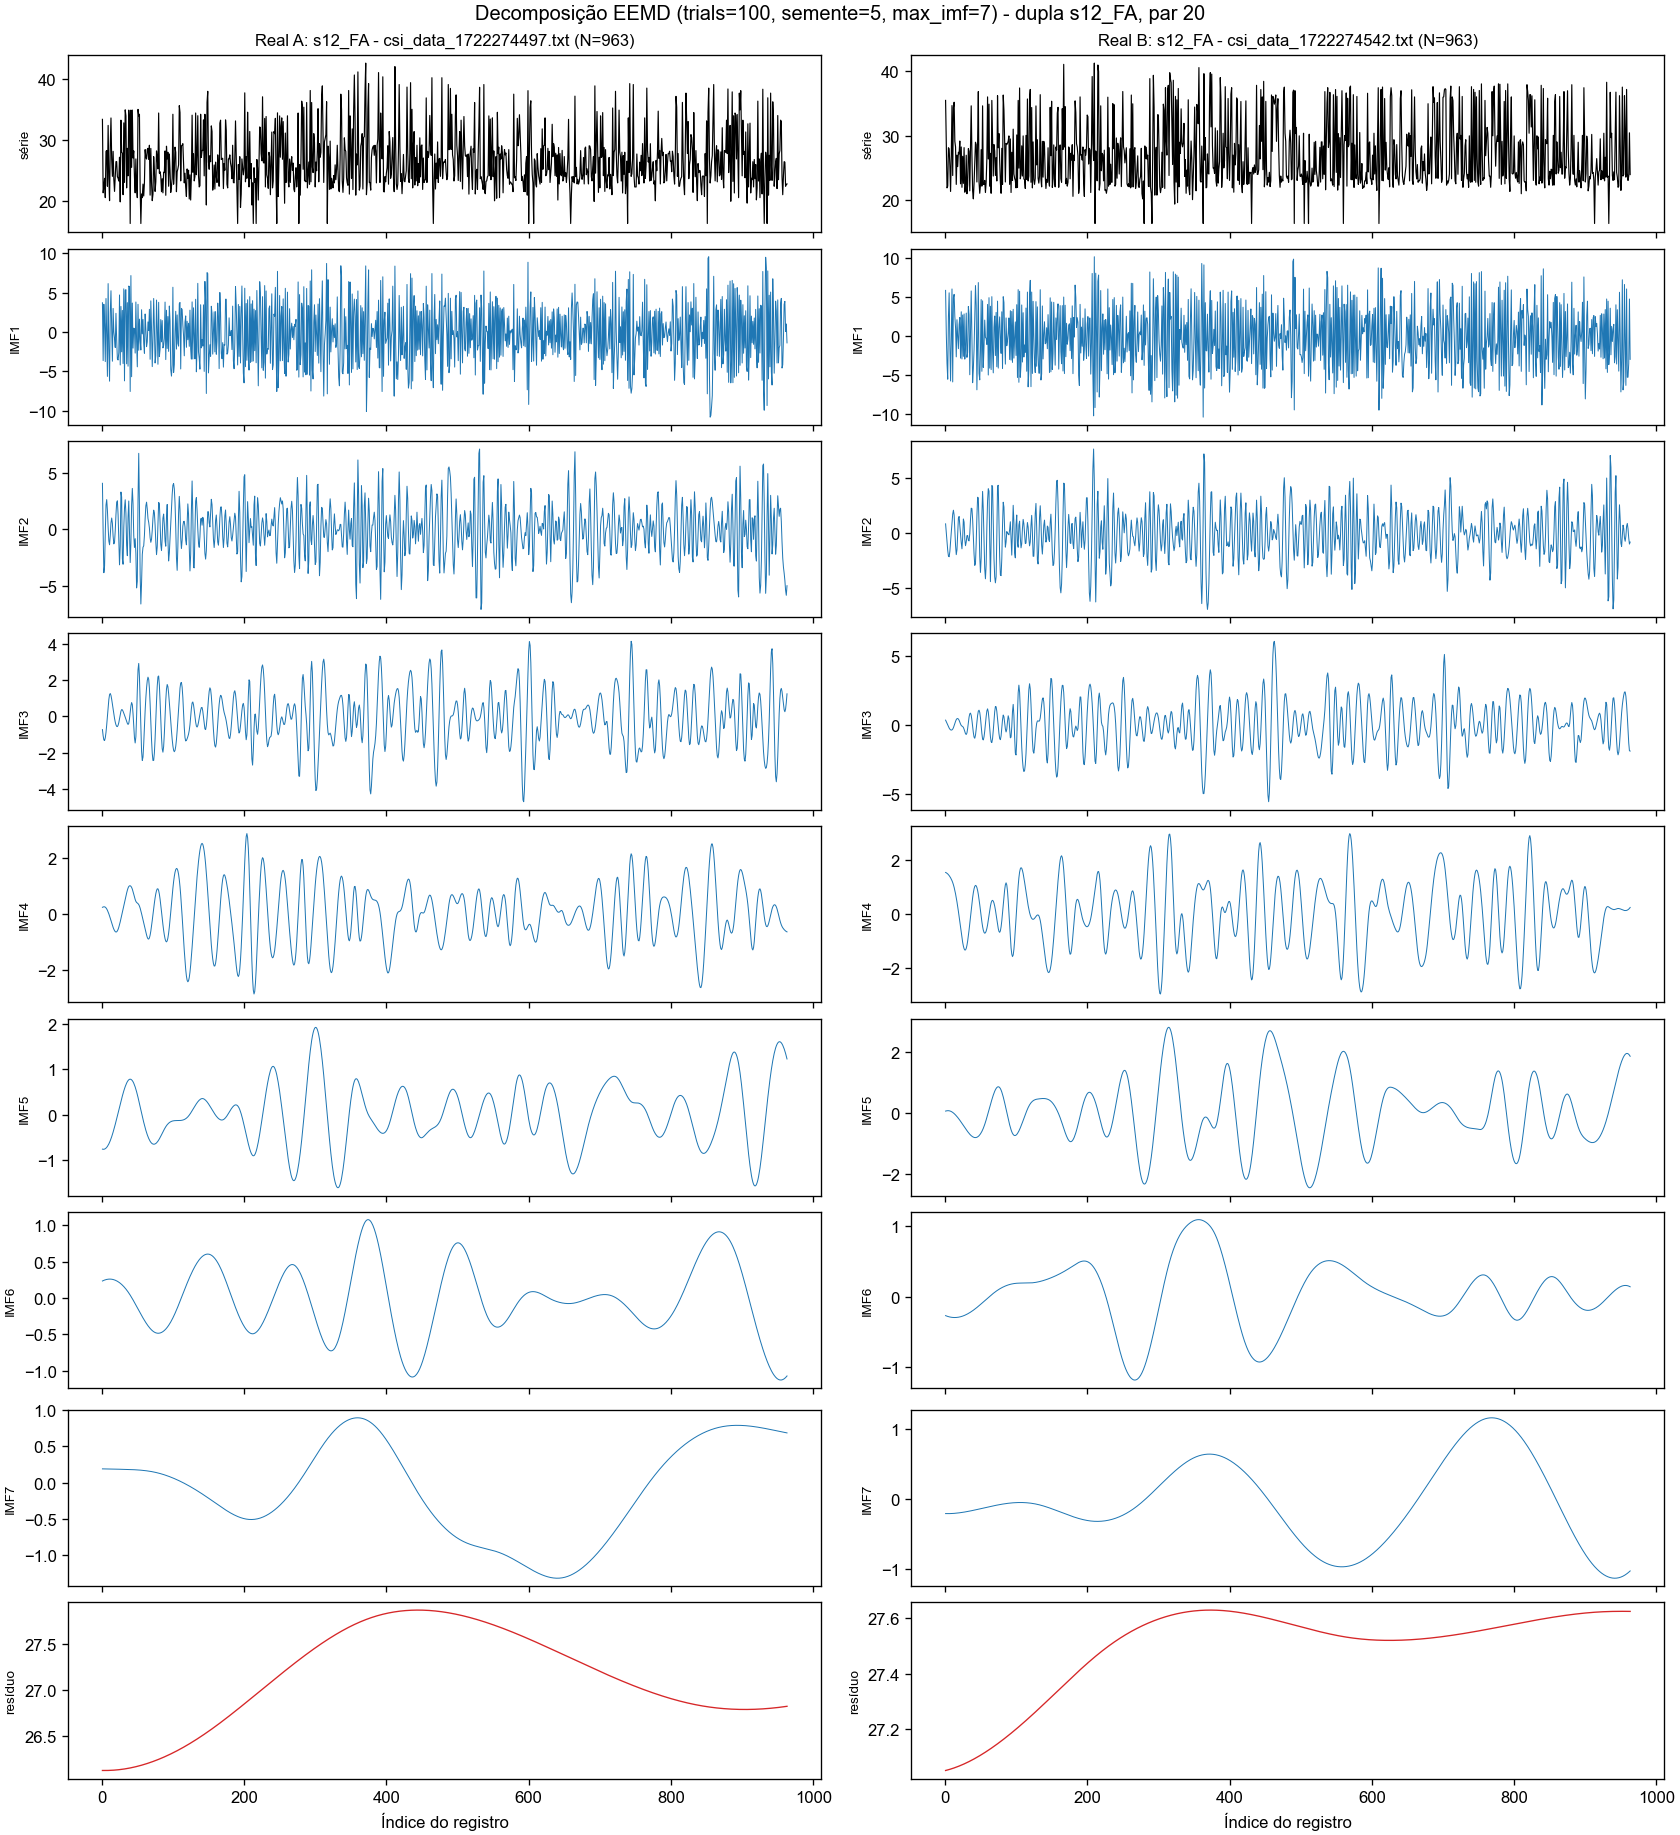
\includegraphics[width=1.00\textwidth,height=19.0cm,keepaspectratio]{Imagens/sec5_decomposicao_s12_FA.png}
    \caption{Decomposição EEMD da dupla s12\_FA (s12, FA): série real do par 20 após o ajuste para N = 963, IMF1 a IMF7 e resíduo. Esquerda: A = Datasets/Activity/FA/s12/csi\_data\_1722274497.txt; direita: B = Datasets/Activity/FA/s12/csi\_data\_1722274542.txt. (arquivo: figuras/sec5\_decomposicao\_s12\_FA.png)}
    \label{fig:sec5_decomposicao_s12_FA}
\end{figure}

\subsection{Comparação entre sinais reais e sintéticos}

As Figuras 12 a 26 mostram, para cada dupla, Real A, Real B e o sinal sintético alinhados verticalmente, com os mesmos limites nos dois eixos dos três gráficos.

\begin{figure}[H]
    \centering
    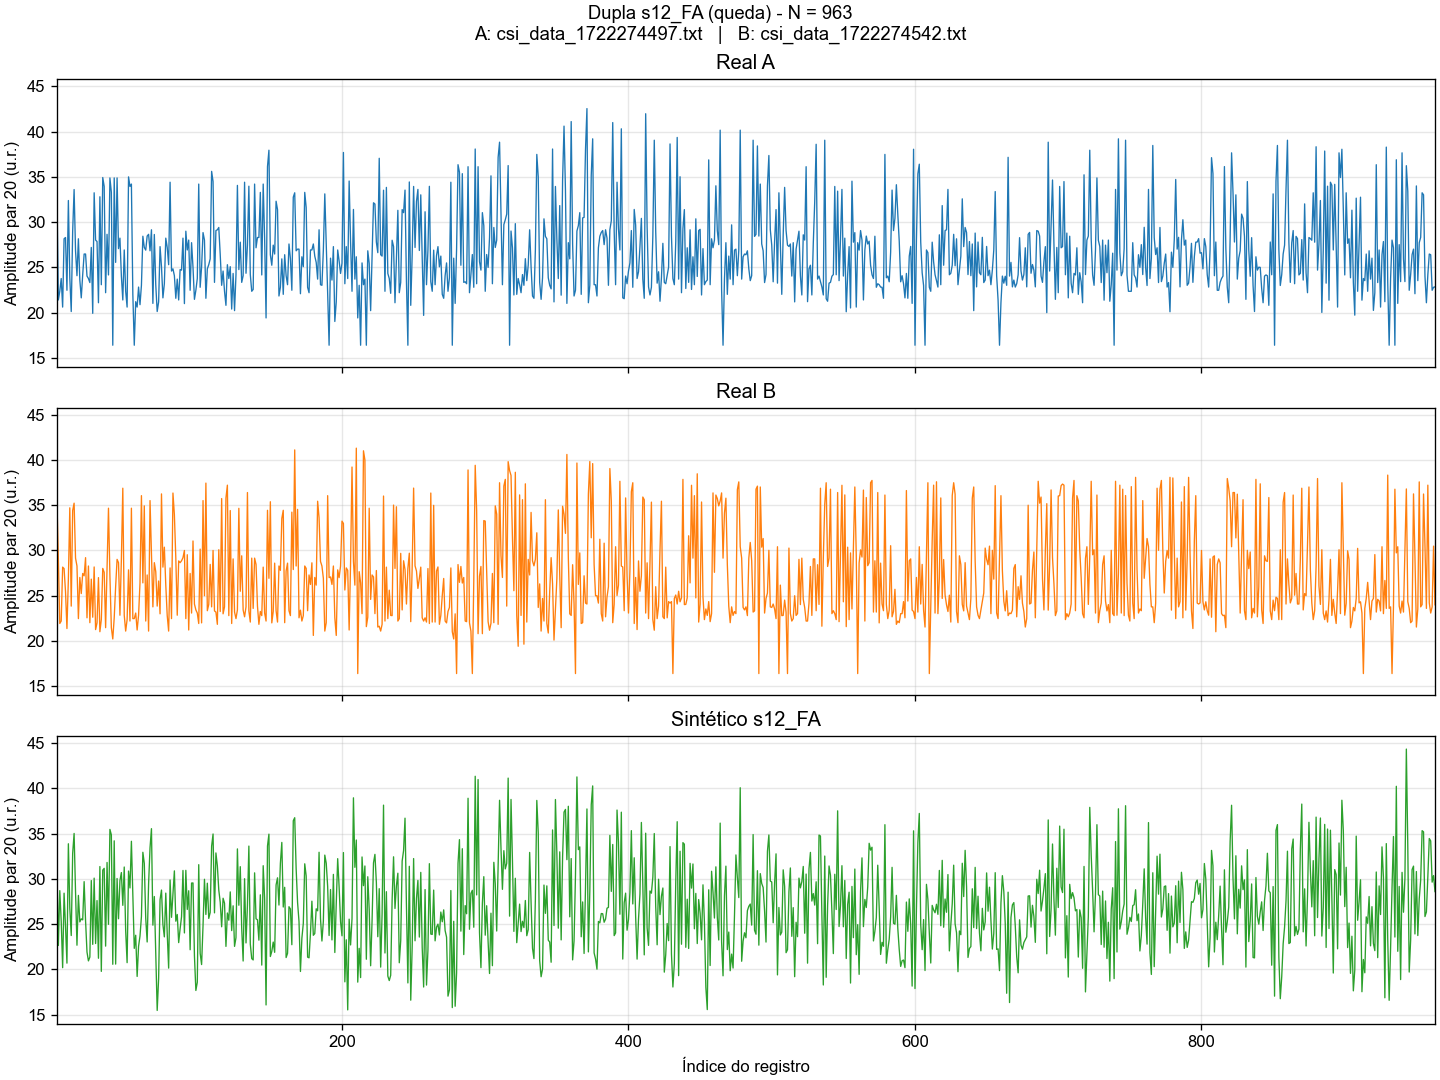
\includegraphics[width=0.79\textwidth,height=19.0cm,keepaspectratio]{Imagens/sec5_comparacao_s12_FA.png}
    \caption{Dupla s12\_FA: Real A (csi\_data\_1722274497.txt), Real B (csi\_data\_1722274542.txt) e Sintético s12\_FA, N = 963. (arquivo: figuras/sec5\_comparacao\_s12\_FA.png)}
    \label{fig:sec5_comparacao_s12_FA}
\end{figure}

\begin{figure}[H]
    \centering
    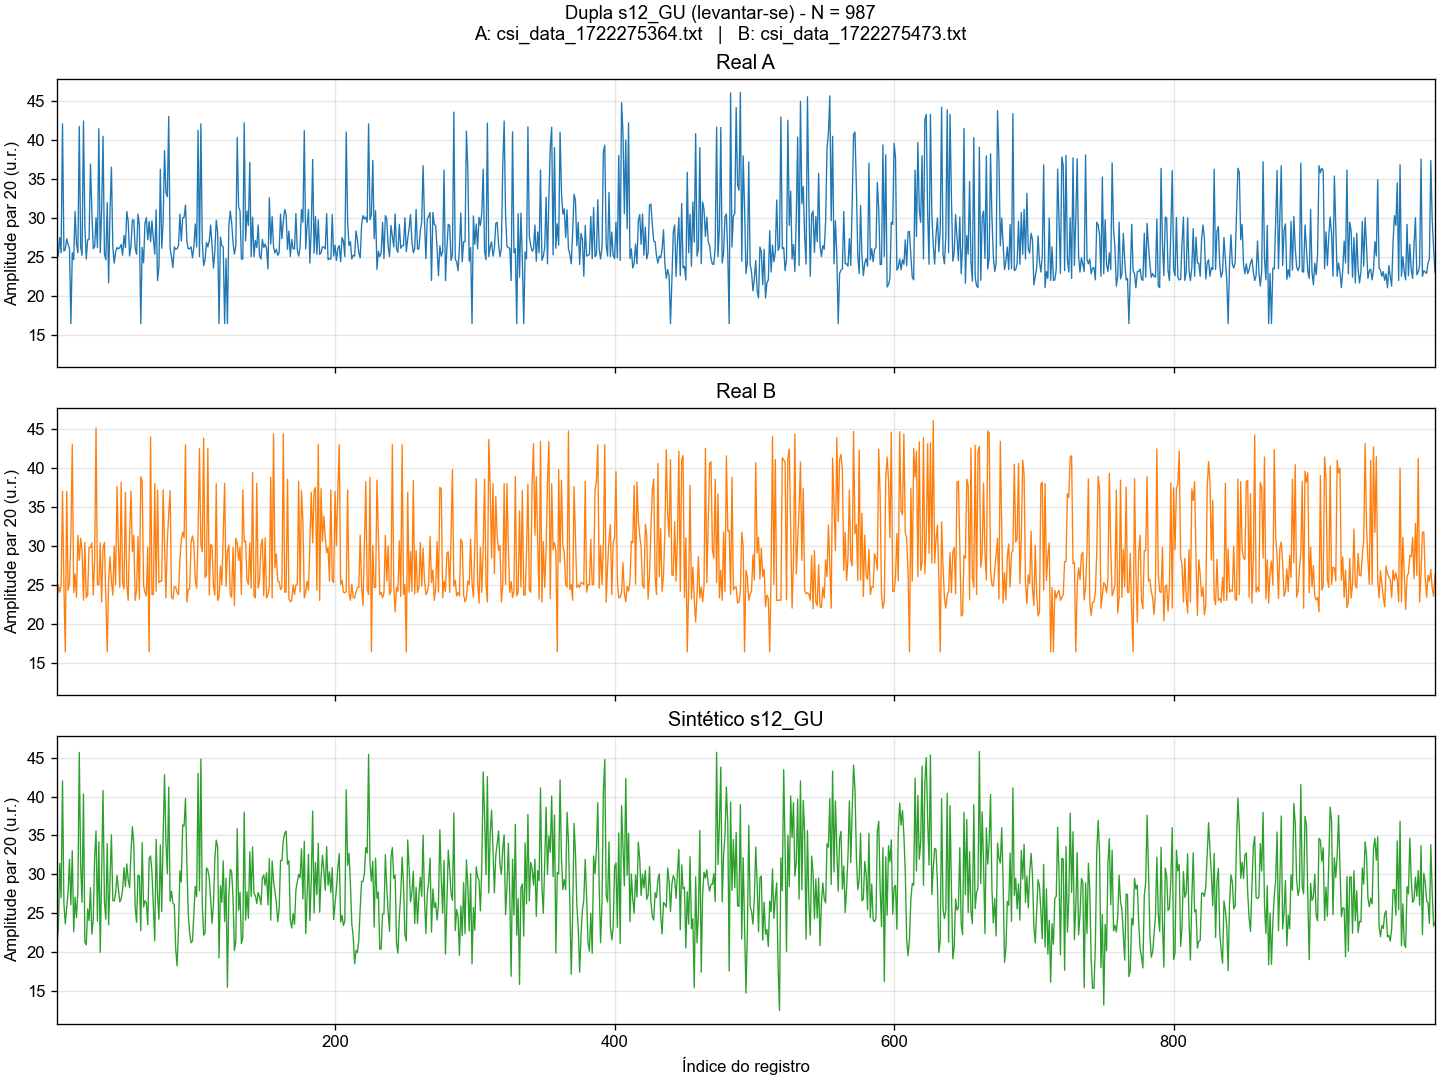
\includegraphics[width=0.79\textwidth,height=19.0cm,keepaspectratio]{Imagens/sec5_comparacao_s12_GU.png}
    \caption{Dupla s12\_GU: Real A (csi\_data\_1722275364.txt), Real B (csi\_data\_1722275473.txt) e Sintético s12\_GU, N = 987. (arquivo: figuras/sec5\_comparacao\_s12\_GU.png)}
    \label{fig:sec5_comparacao_s12_GU}
\end{figure}

\begin{figure}[H]
    \centering
    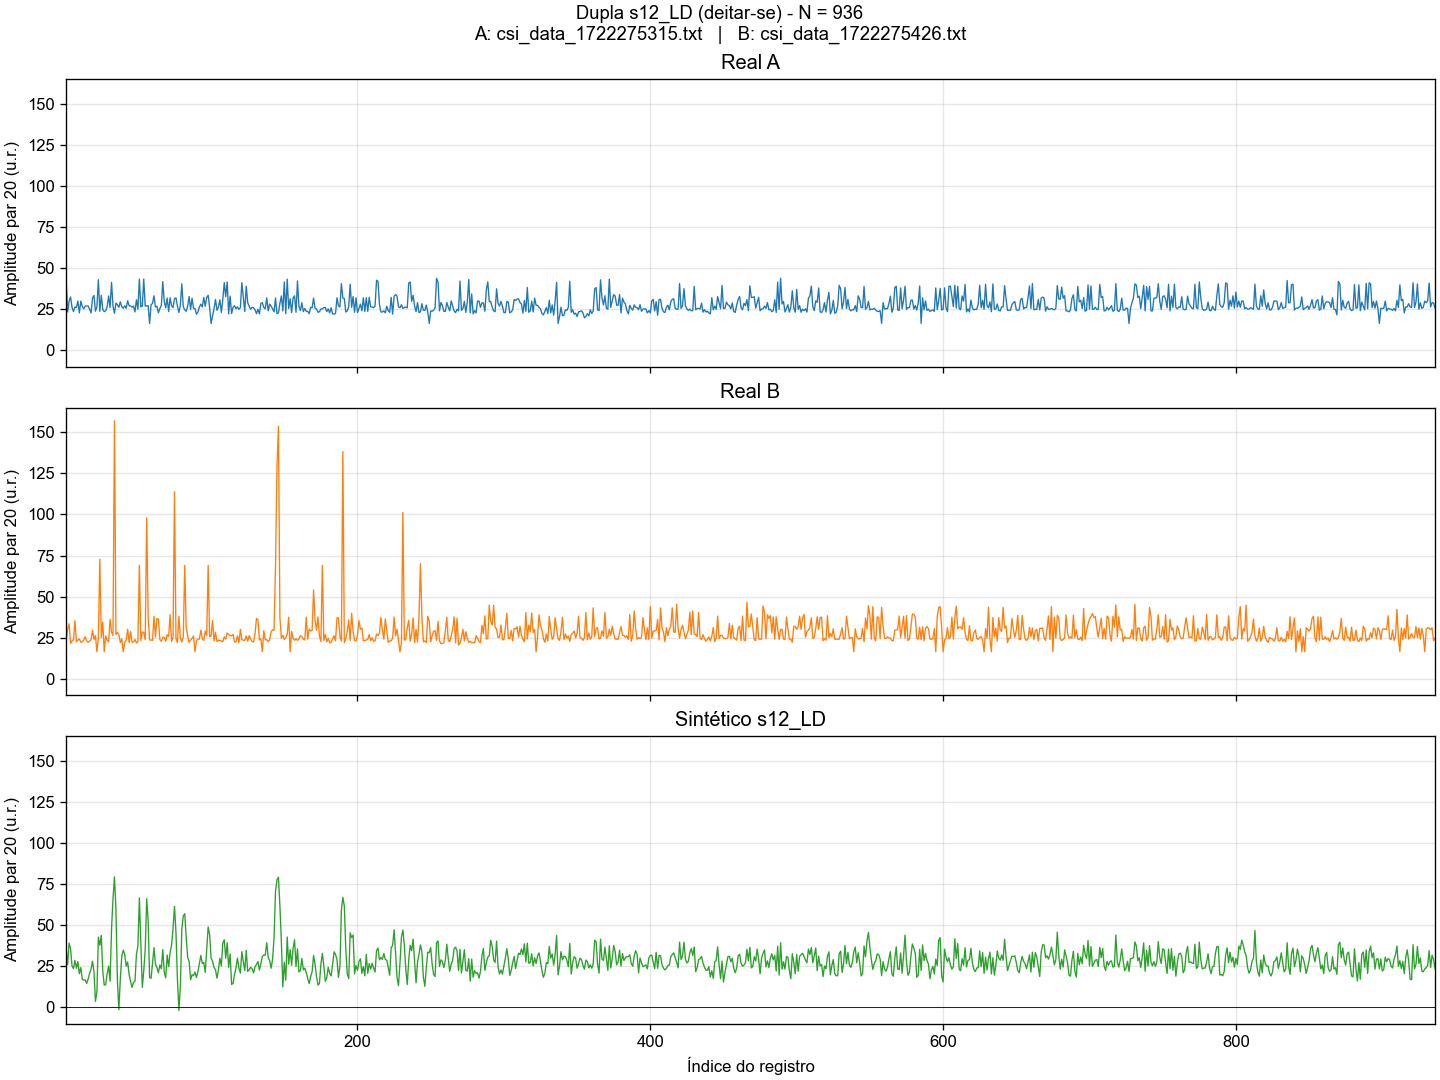
\includegraphics[width=0.79\textwidth,height=19.0cm,keepaspectratio]{Imagens/sec5_comparacao_s12_LD.png}
    \caption{Dupla s12\_LD: Real A (csi\_data\_1722275315.txt), Real B (csi\_data\_1722275426.txt) e Sintético s12\_LD, N = 936. (arquivo: figuras/sec5\_comparacao\_s12\_LD.png)}
    \label{fig:sec5_comparacao_s12_LD}
\end{figure}

\begin{figure}[H]
    \centering
    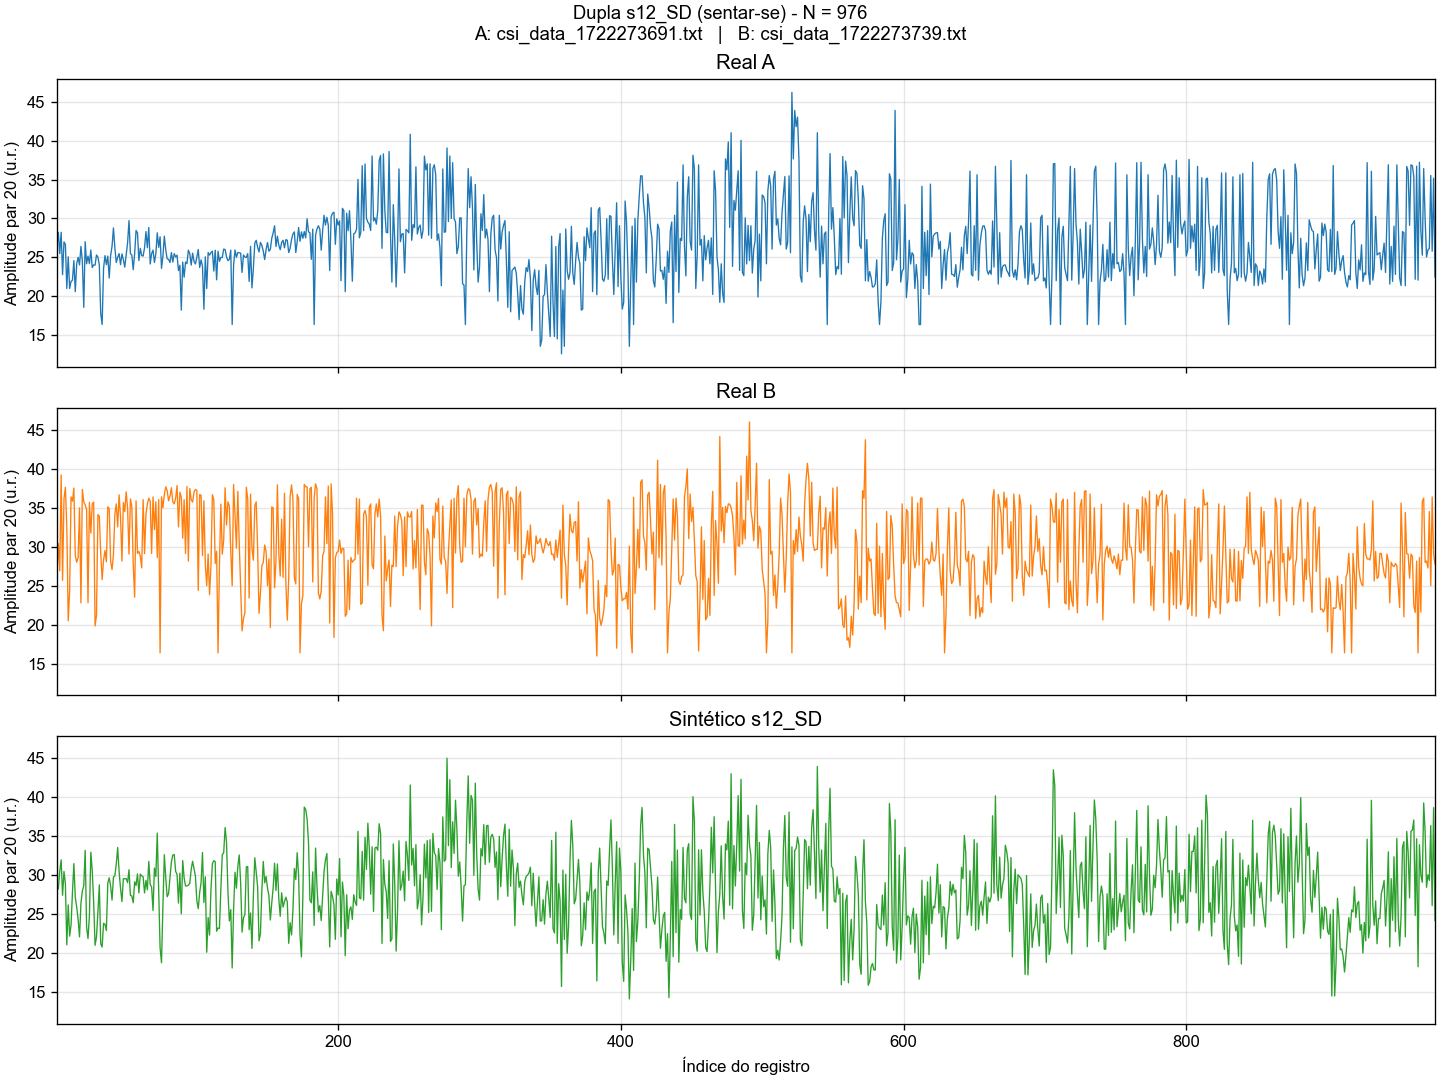
\includegraphics[width=0.79\textwidth,height=19.0cm,keepaspectratio]{Imagens/sec5_comparacao_s12_SD.png}
    \caption{Dupla s12\_SD: Real A (csi\_data\_1722273691.txt), Real B (csi\_data\_1722273739.txt) e Sintético s12\_SD, N = 976. (arquivo: figuras/sec5\_comparacao\_s12\_SD.png)}
    \label{fig:sec5_comparacao_s12_SD}
\end{figure}

\begin{figure}[H]
    \centering
    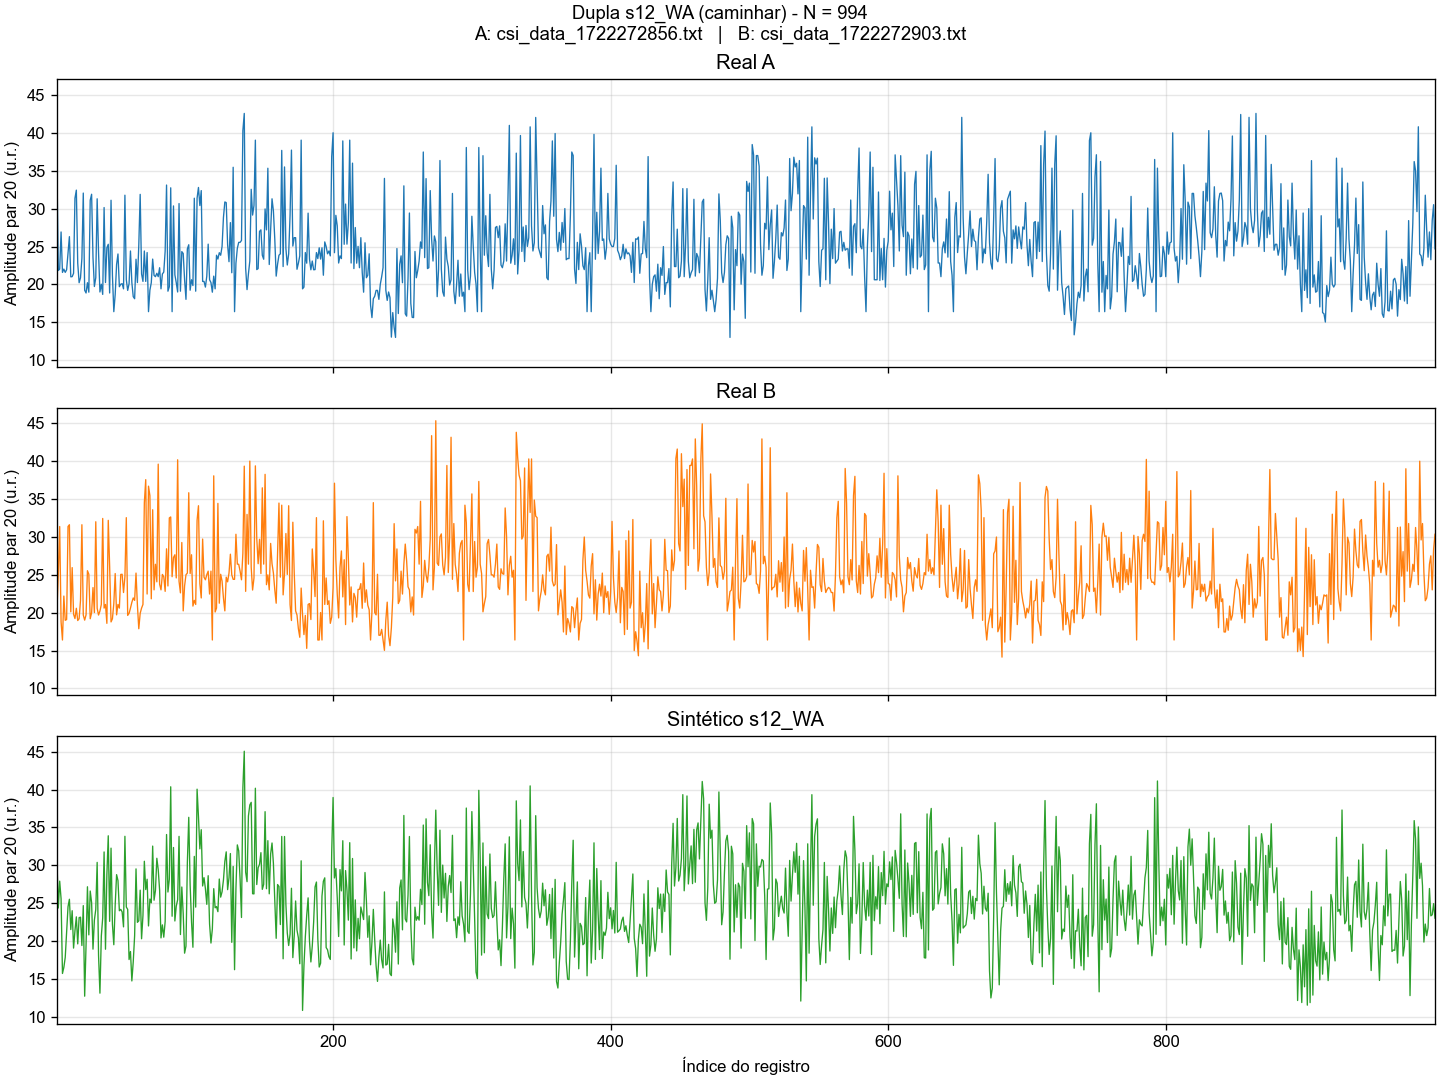
\includegraphics[width=0.79\textwidth,height=19.0cm,keepaspectratio]{Imagens/sec5_comparacao_s12_WA.png}
    \caption{Dupla s12\_WA: Real A (csi\_data\_1722272856.txt), Real B (csi\_data\_1722272903.txt) e Sintético s12\_WA, N = 994. (arquivo: figuras/sec5\_comparacao\_s12\_WA.png)}
    \label{fig:sec5_comparacao_s12_WA}
\end{figure}

\begin{figure}[H]
    \centering
    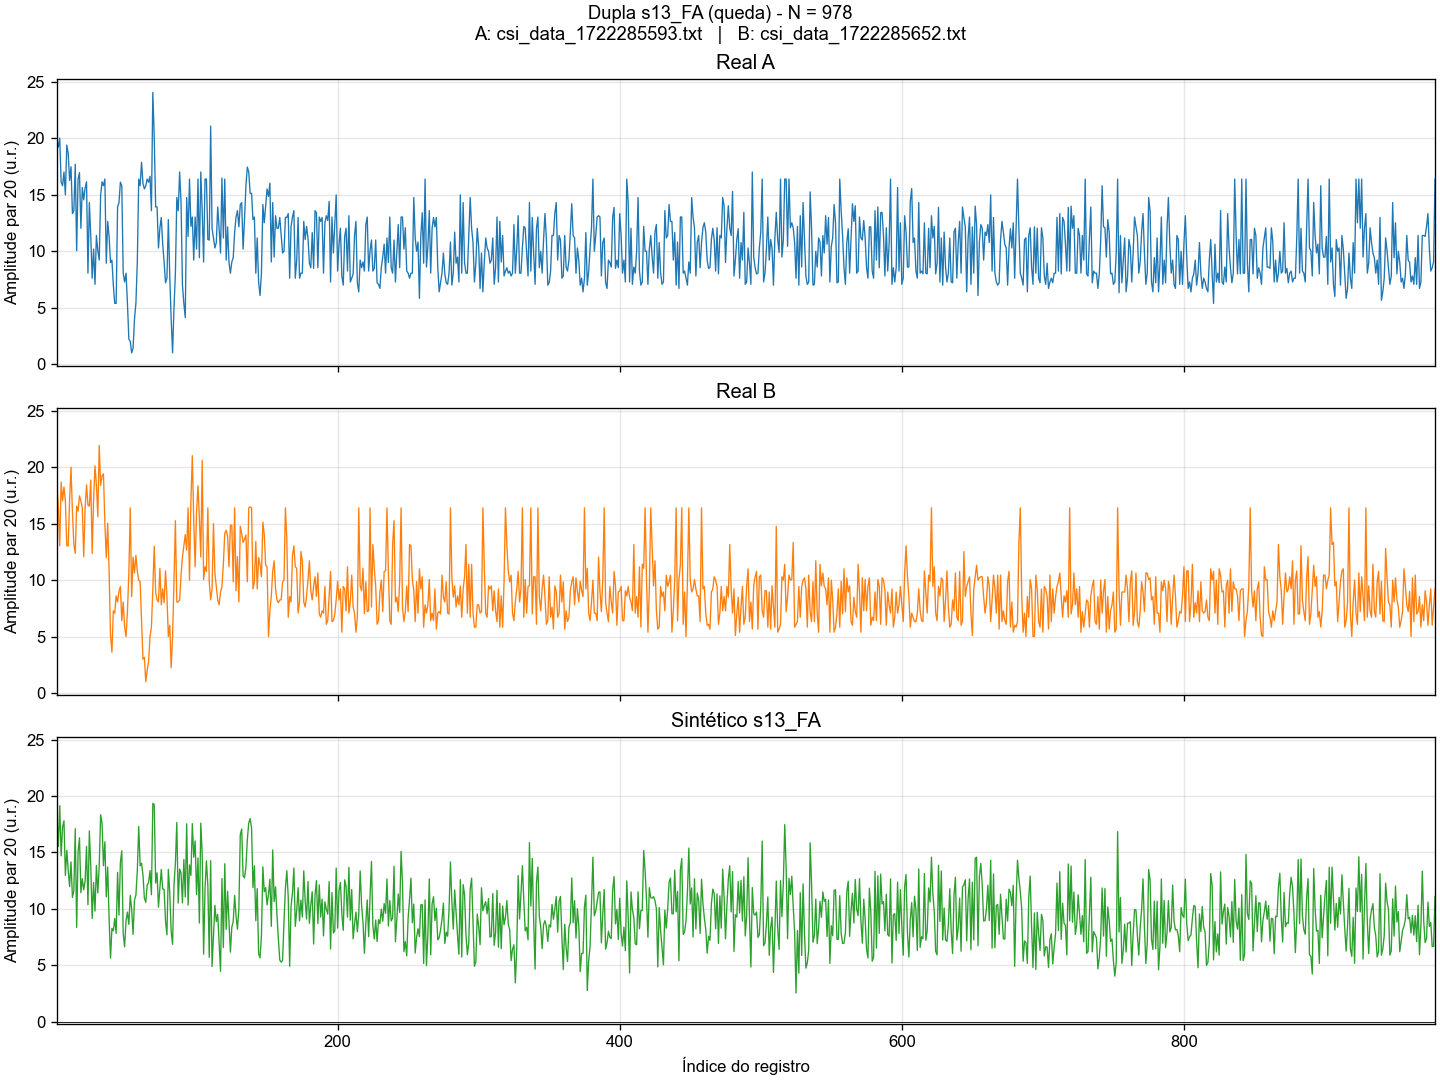
\includegraphics[width=0.79\textwidth,height=19.0cm,keepaspectratio]{Imagens/sec5_comparacao_s13_FA.png}
    \caption{Dupla s13\_FA: Real A (csi\_data\_1722285593.txt), Real B (csi\_data\_1722285652.txt) e Sintético s13\_FA, N = 978. (arquivo: figuras/sec5\_comparacao\_s13\_FA.png)}
    \label{fig:sec5_comparacao_s13_FA}
\end{figure}

\begin{figure}[H]
    \centering
    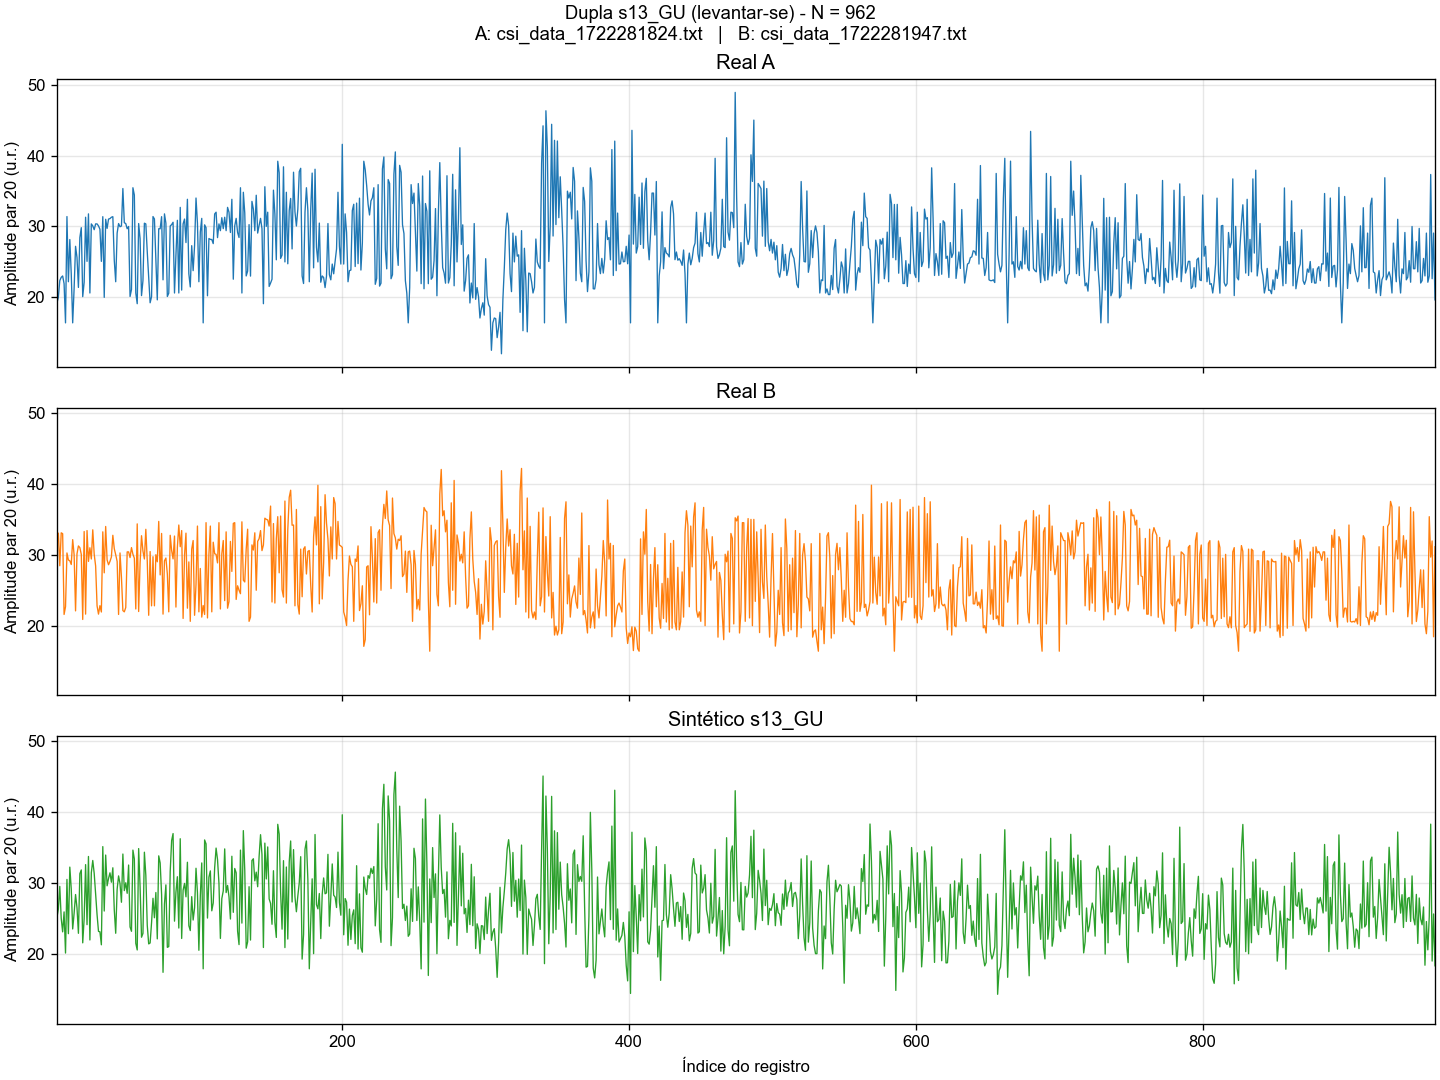
\includegraphics[width=0.79\textwidth,height=19.0cm,keepaspectratio]{Imagens/sec5_comparacao_s13_GU.png}
    \caption{Dupla s13\_GU: Real A (csi\_data\_1722281824.txt), Real B (csi\_data\_1722281947.txt) e Sintético s13\_GU, N = 962. (arquivo: figuras/sec5\_comparacao\_s13\_GU.png)}
    \label{fig:sec5_comparacao_s13_GU}
\end{figure}

\begin{figure}[H]
    \centering
    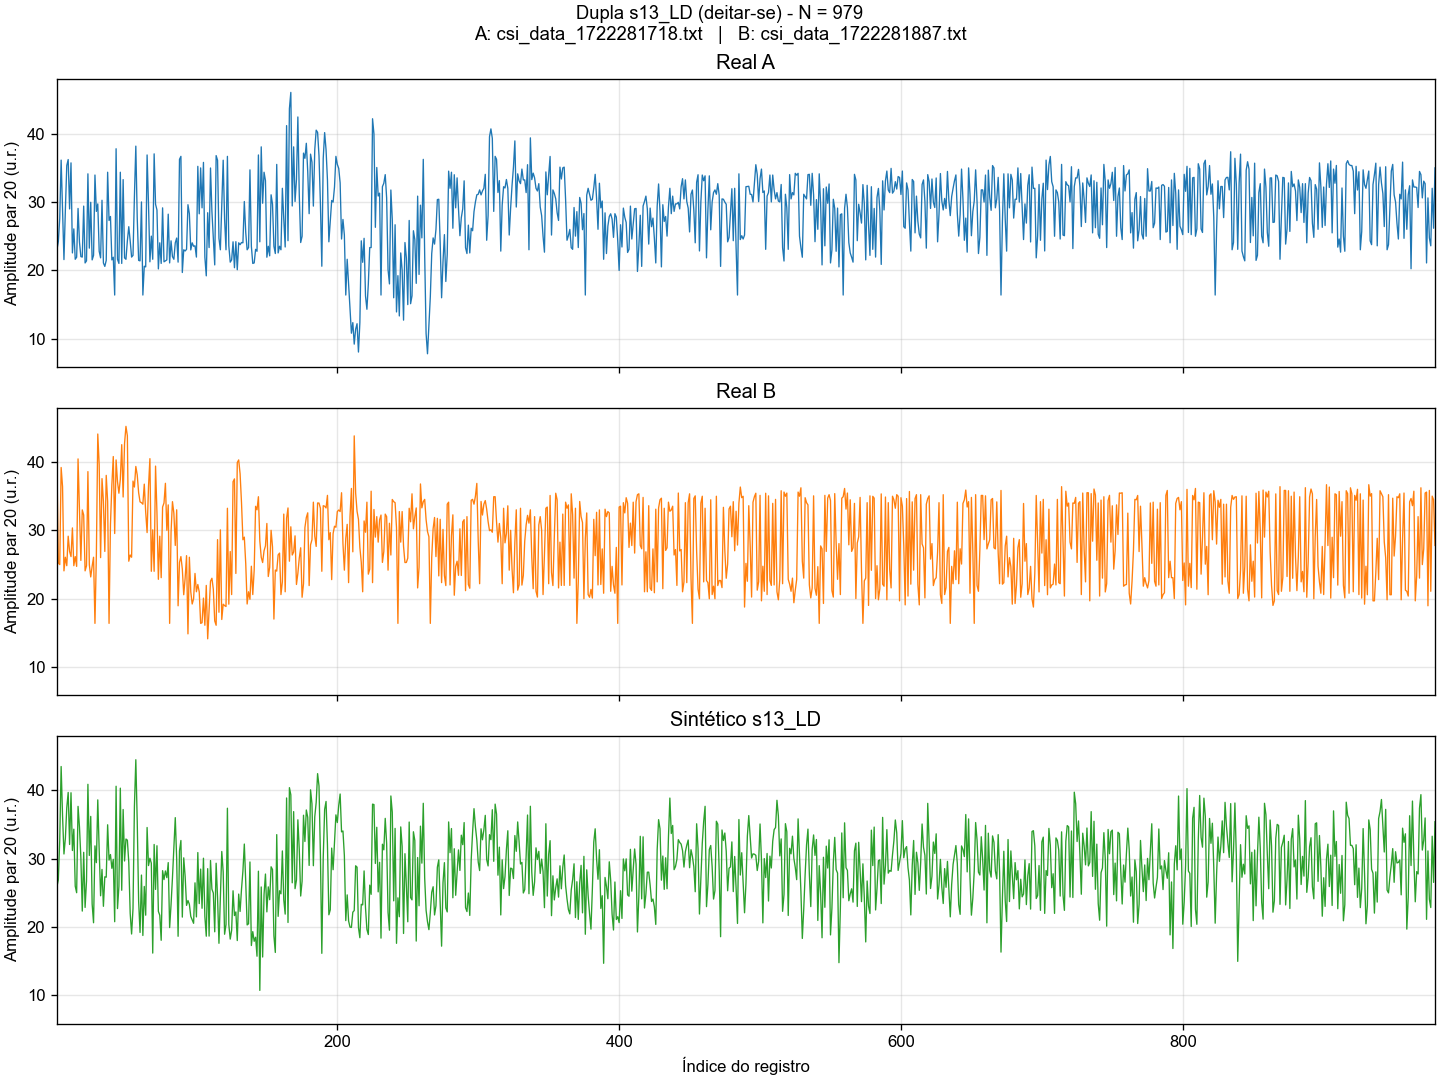
\includegraphics[width=0.79\textwidth,height=19.0cm,keepaspectratio]{Imagens/sec5_comparacao_s13_LD.png}
    \caption{Dupla s13\_LD: Real A (csi\_data\_1722281718.txt), Real B (csi\_data\_1722281887.txt) e Sintético s13\_LD, N = 979. (arquivo: figuras/sec5\_comparacao\_s13\_LD.png)}
    \label{fig:sec5_comparacao_s13_LD}
\end{figure}

\begin{figure}[H]
    \centering
    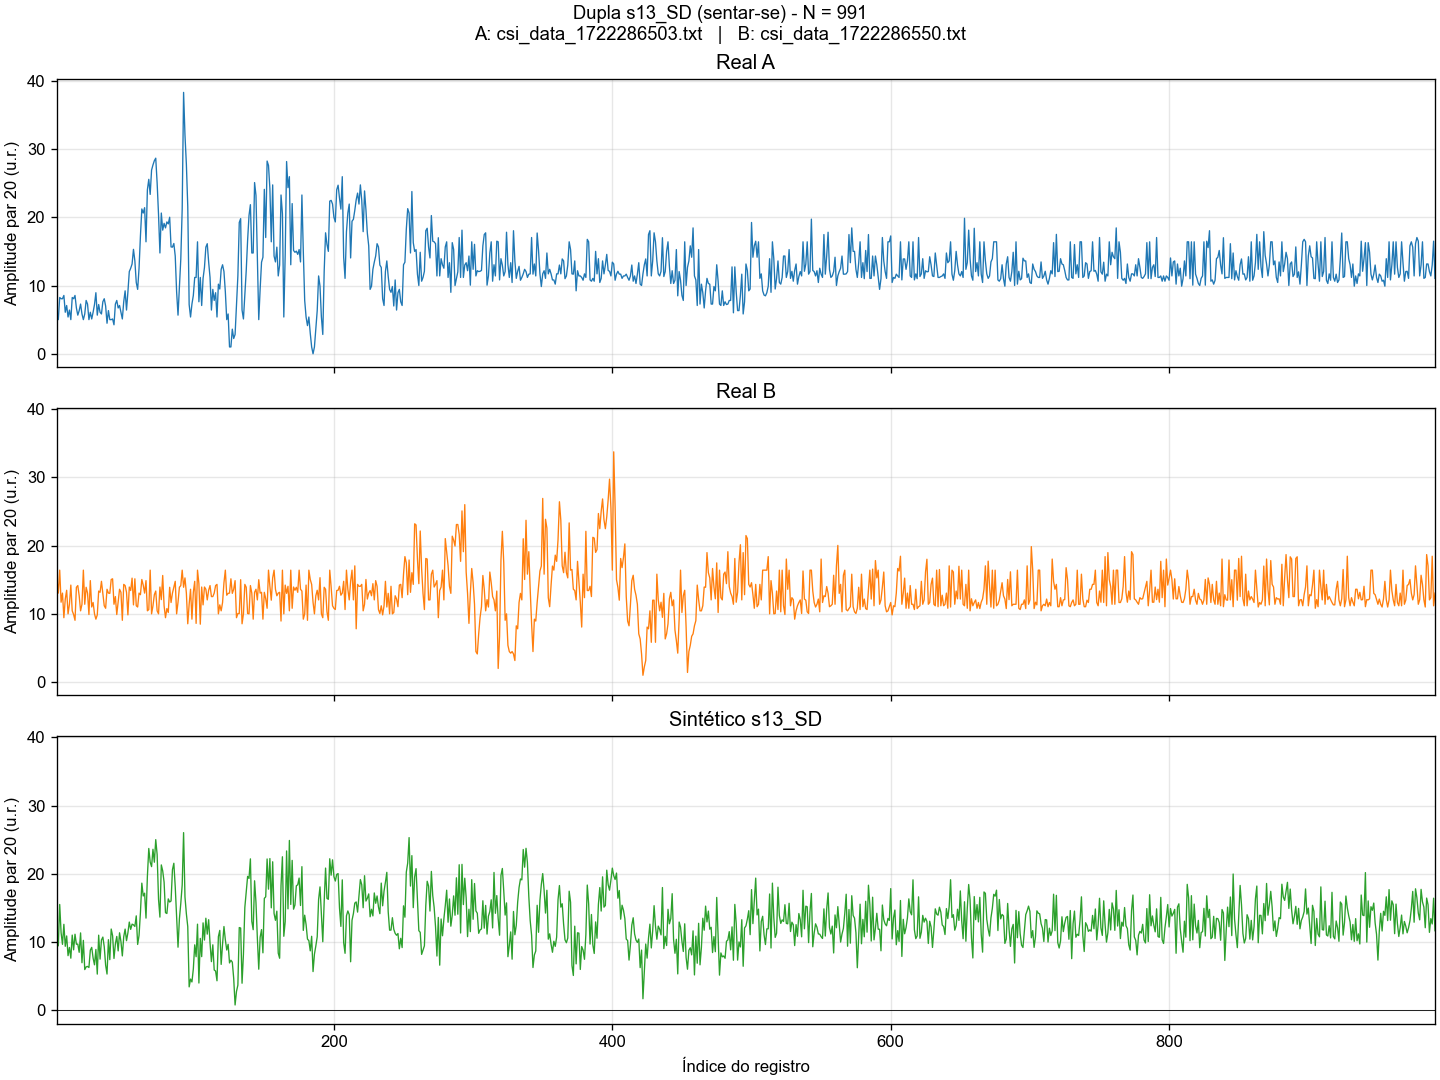
\includegraphics[width=0.79\textwidth,height=19.0cm,keepaspectratio]{Imagens/sec5_comparacao_s13_SD.png}
    \caption{Dupla s13\_SD: Real A (csi\_data\_1722286503.txt), Real B (csi\_data\_1722286550.txt) e Sintético s13\_SD, N = 991. (arquivo: figuras/sec5\_comparacao\_s13\_SD.png)}
    \label{fig:sec5_comparacao_s13_SD}
\end{figure}

\begin{figure}[H]
    \centering
    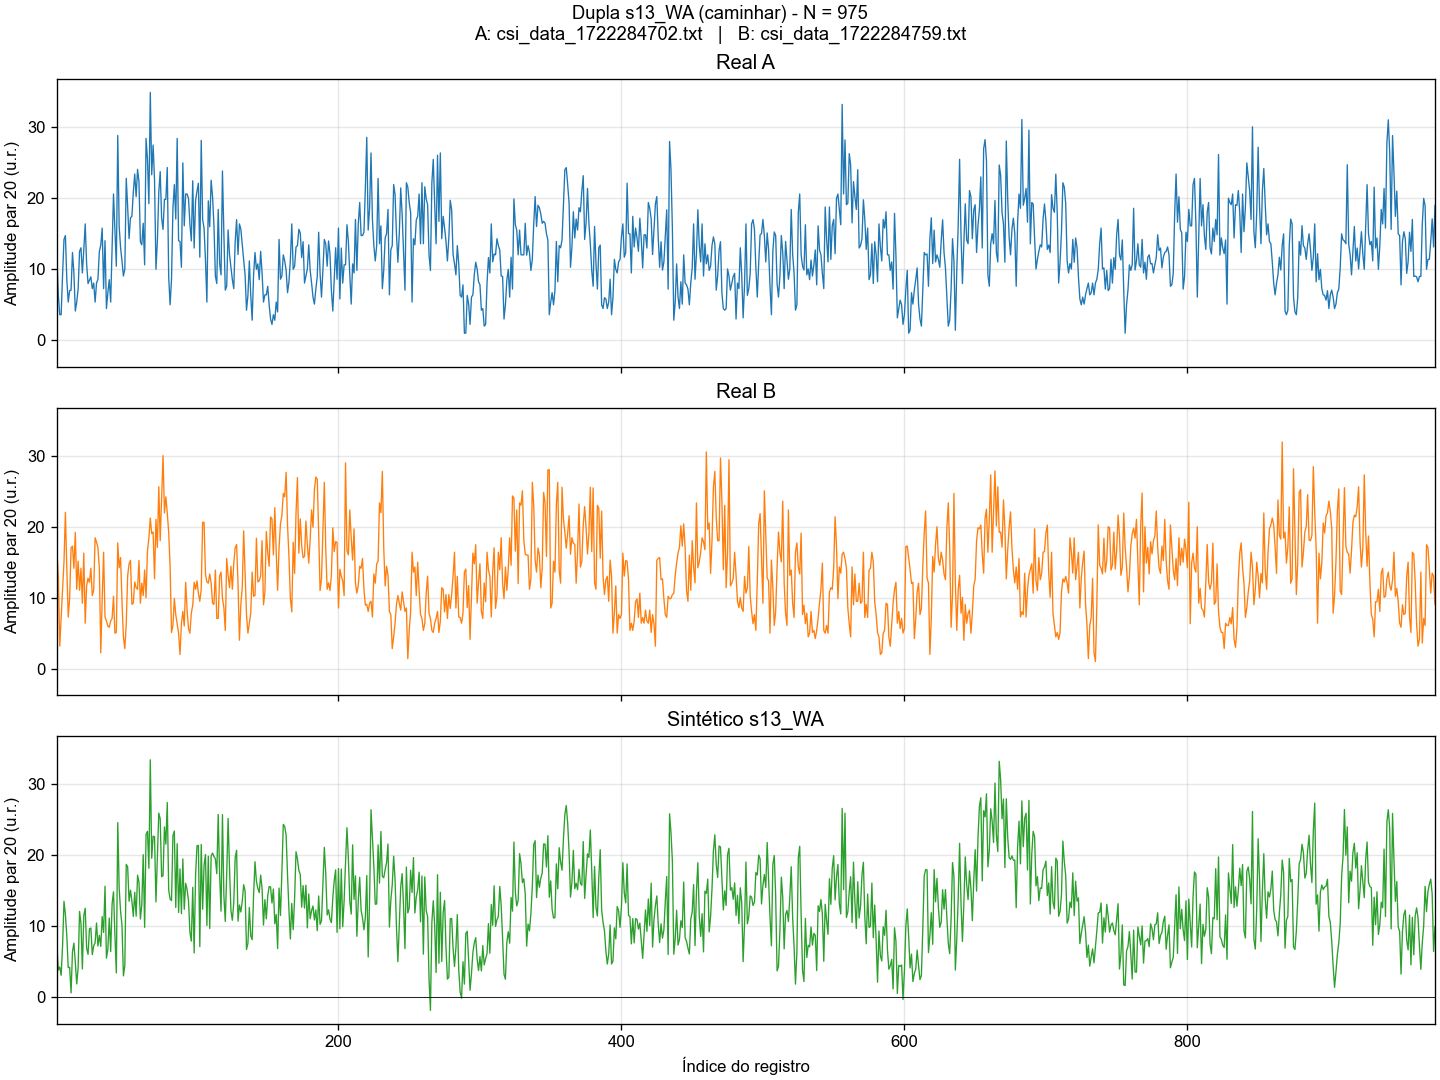
\includegraphics[width=0.79\textwidth,height=19.0cm,keepaspectratio]{Imagens/sec5_comparacao_s13_WA.png}
    \caption{Dupla s13\_WA: Real A (csi\_data\_1722284702.txt), Real B (csi\_data\_1722284759.txt) e Sintético s13\_WA, N = 975. (arquivo: figuras/sec5\_comparacao\_s13\_WA.png)}
    \label{fig:sec5_comparacao_s13_WA}
\end{figure}

\begin{figure}[H]
    \centering
    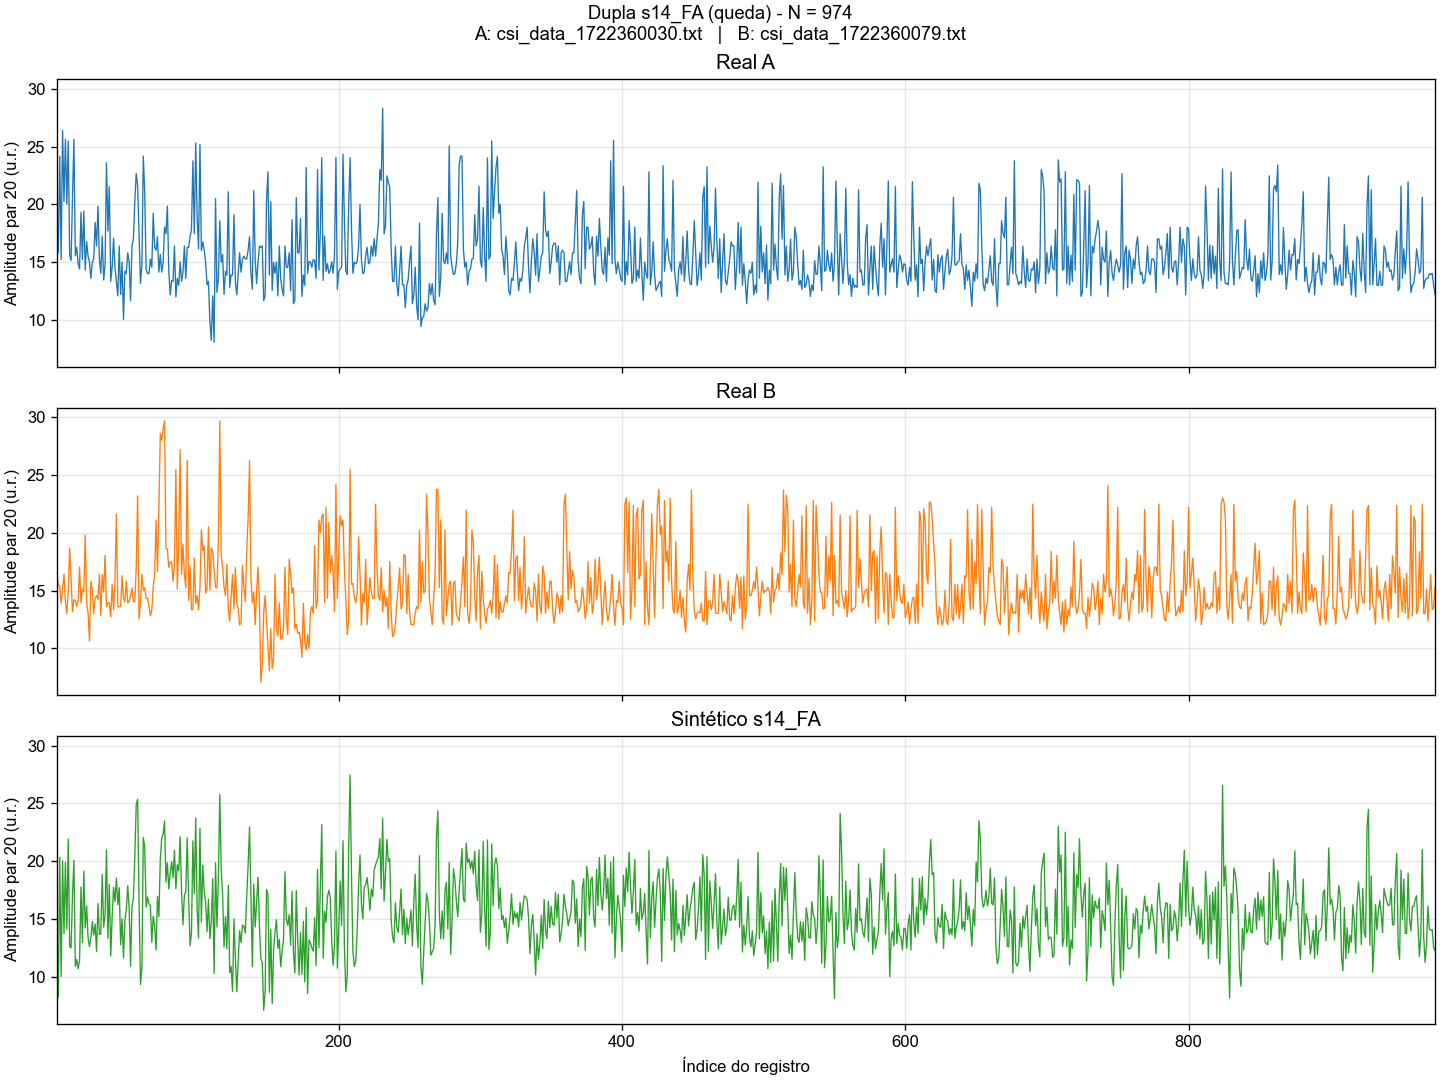
\includegraphics[width=0.79\textwidth,height=19.0cm,keepaspectratio]{Imagens/sec5_comparacao_s14_FA.png}
    \caption{Dupla s14\_FA: Real A (csi\_data\_1722360030.txt), Real B (csi\_data\_1722360079.txt) e Sintético s14\_FA, N = 974. (arquivo: figuras/sec5\_comparacao\_s14\_FA.png)}
    \label{fig:sec5_comparacao_s14_FA}
\end{figure}

\begin{figure}[H]
    \centering
    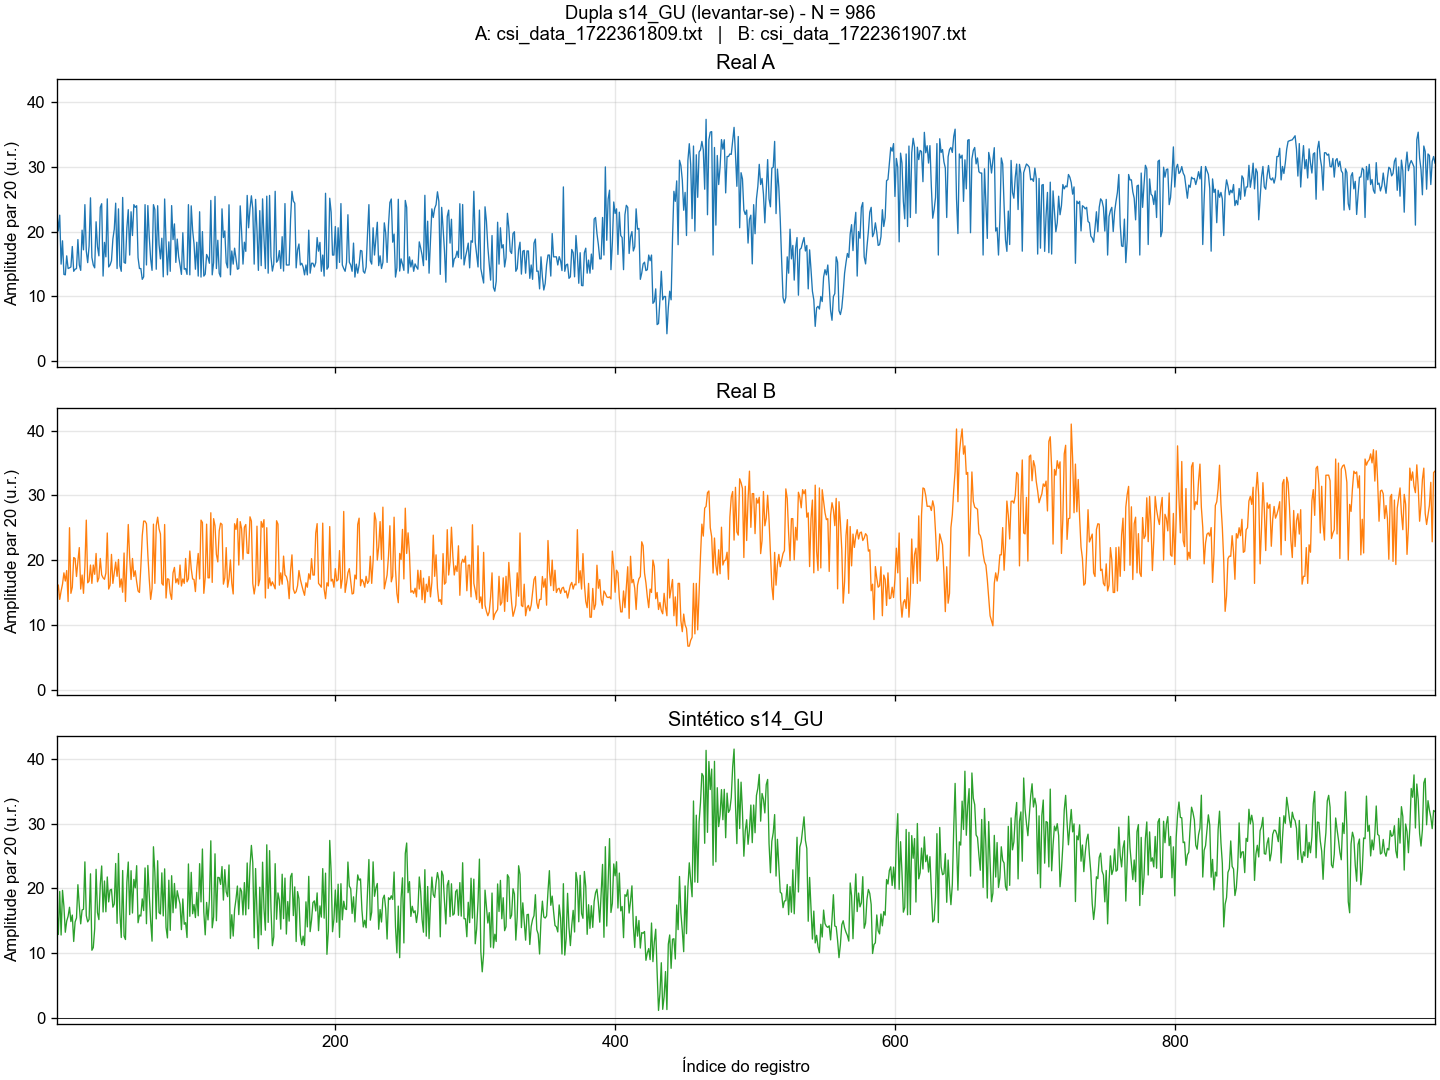
\includegraphics[width=0.79\textwidth,height=19.0cm,keepaspectratio]{Imagens/sec5_comparacao_s14_GU.png}
    \caption{Dupla s14\_GU: Real A (csi\_data\_1722361809.txt), Real B (csi\_data\_1722361907.txt) e Sintético s14\_GU, N = 986. (arquivo: figuras/sec5\_comparacao\_s14\_GU.png)}
    \label{fig:sec5_comparacao_s14_GU}
\end{figure}

\begin{figure}[H]
    \centering
    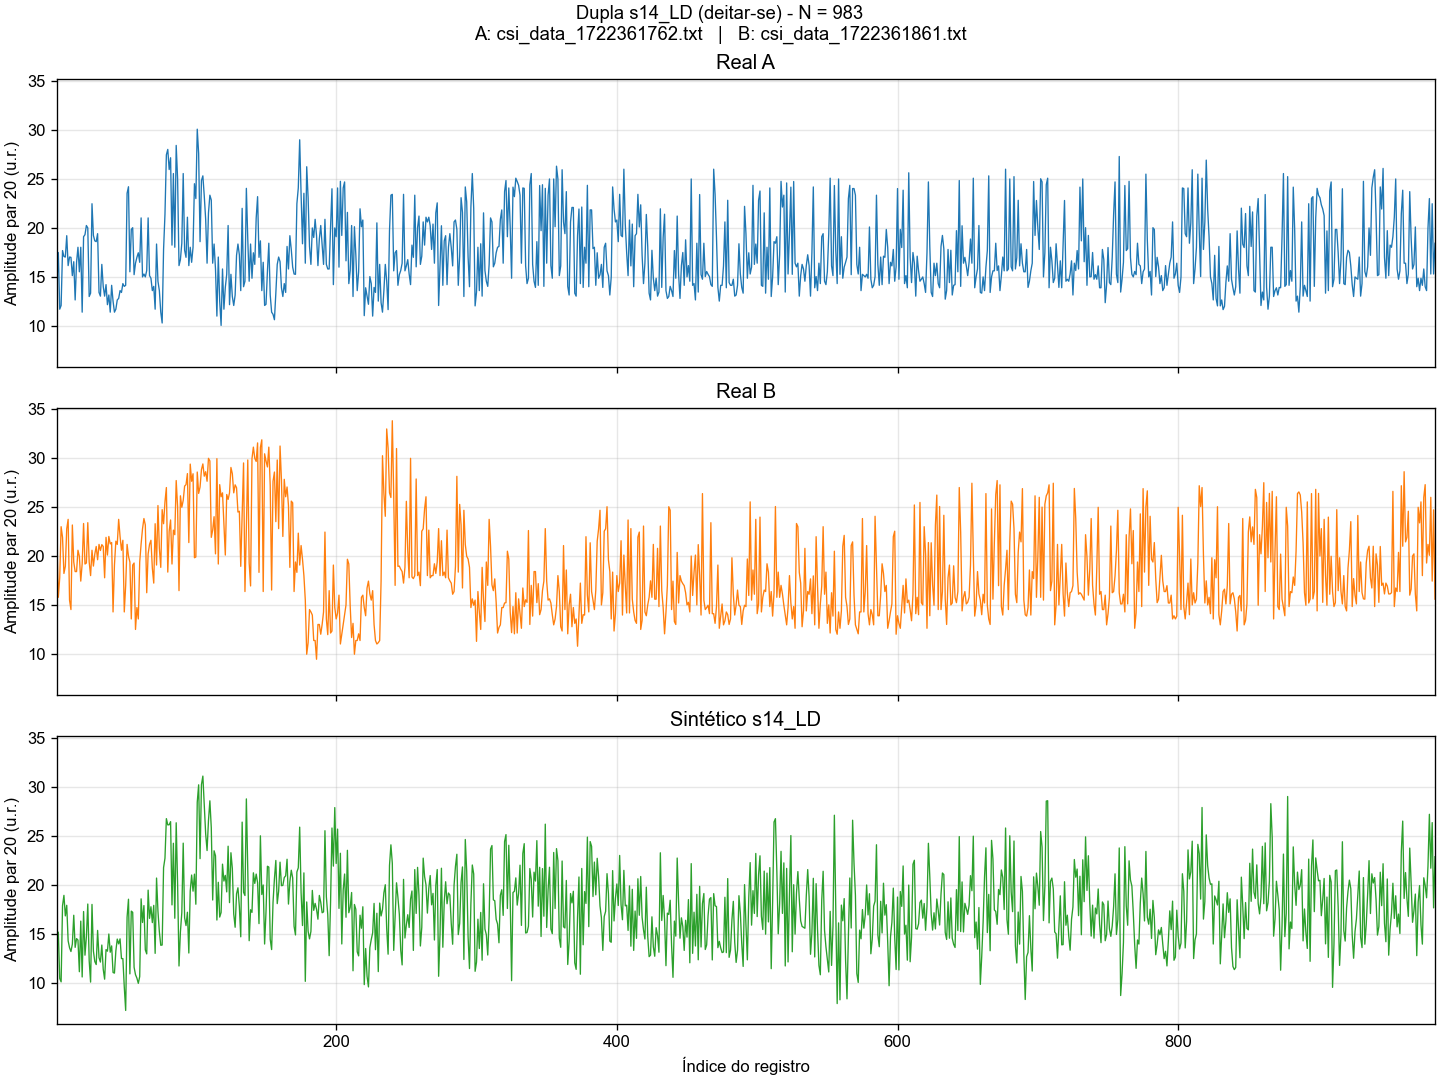
\includegraphics[width=0.79\textwidth,height=19.0cm,keepaspectratio]{Imagens/sec5_comparacao_s14_LD.png}
    \caption{Dupla s14\_LD: Real A (csi\_data\_1722361762.txt), Real B (csi\_data\_1722361861.txt) e Sintético s14\_LD, N = 983. (arquivo: figuras/sec5\_comparacao\_s14\_LD.png)}
    \label{fig:sec5_comparacao_s14_LD}
\end{figure}

\begin{figure}[H]
    \centering
    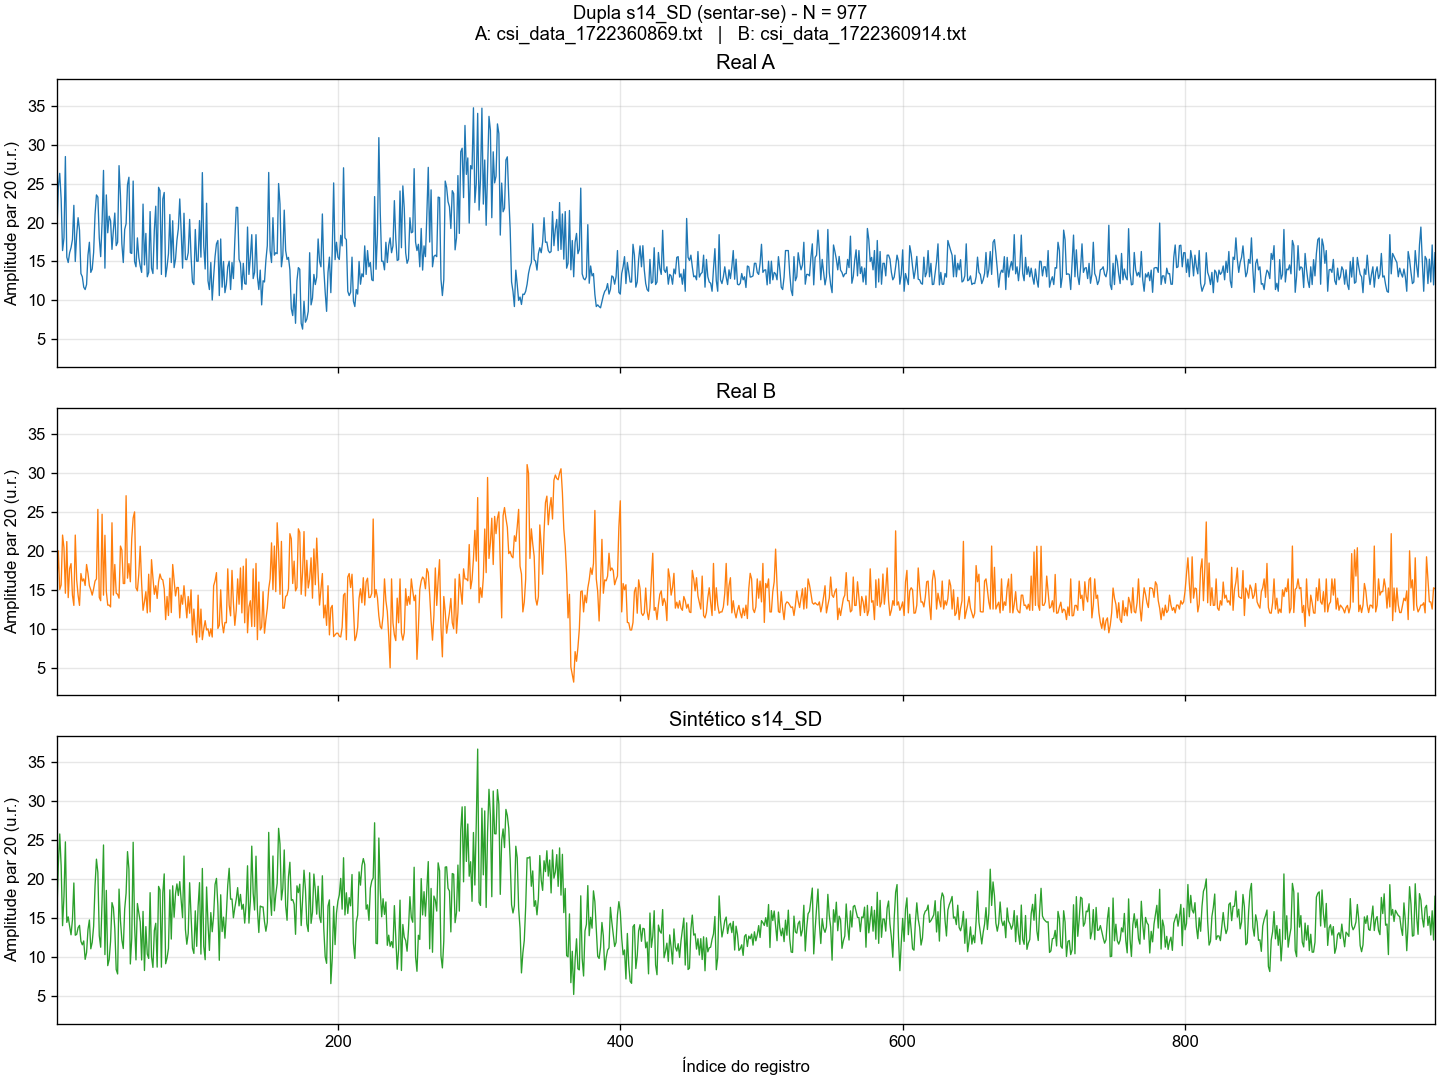
\includegraphics[width=0.79\textwidth,height=19.0cm,keepaspectratio]{Imagens/sec5_comparacao_s14_SD.png}
    \caption{Dupla s14\_SD: Real A (csi\_data\_1722360869.txt), Real B (csi\_data\_1722360914.txt) e Sintético s14\_SD, N = 977. (arquivo: figuras/sec5\_comparacao\_s14\_SD.png)}
    \label{fig:sec5_comparacao_s14_SD}
\end{figure}

\begin{figure}[H]
    \centering
    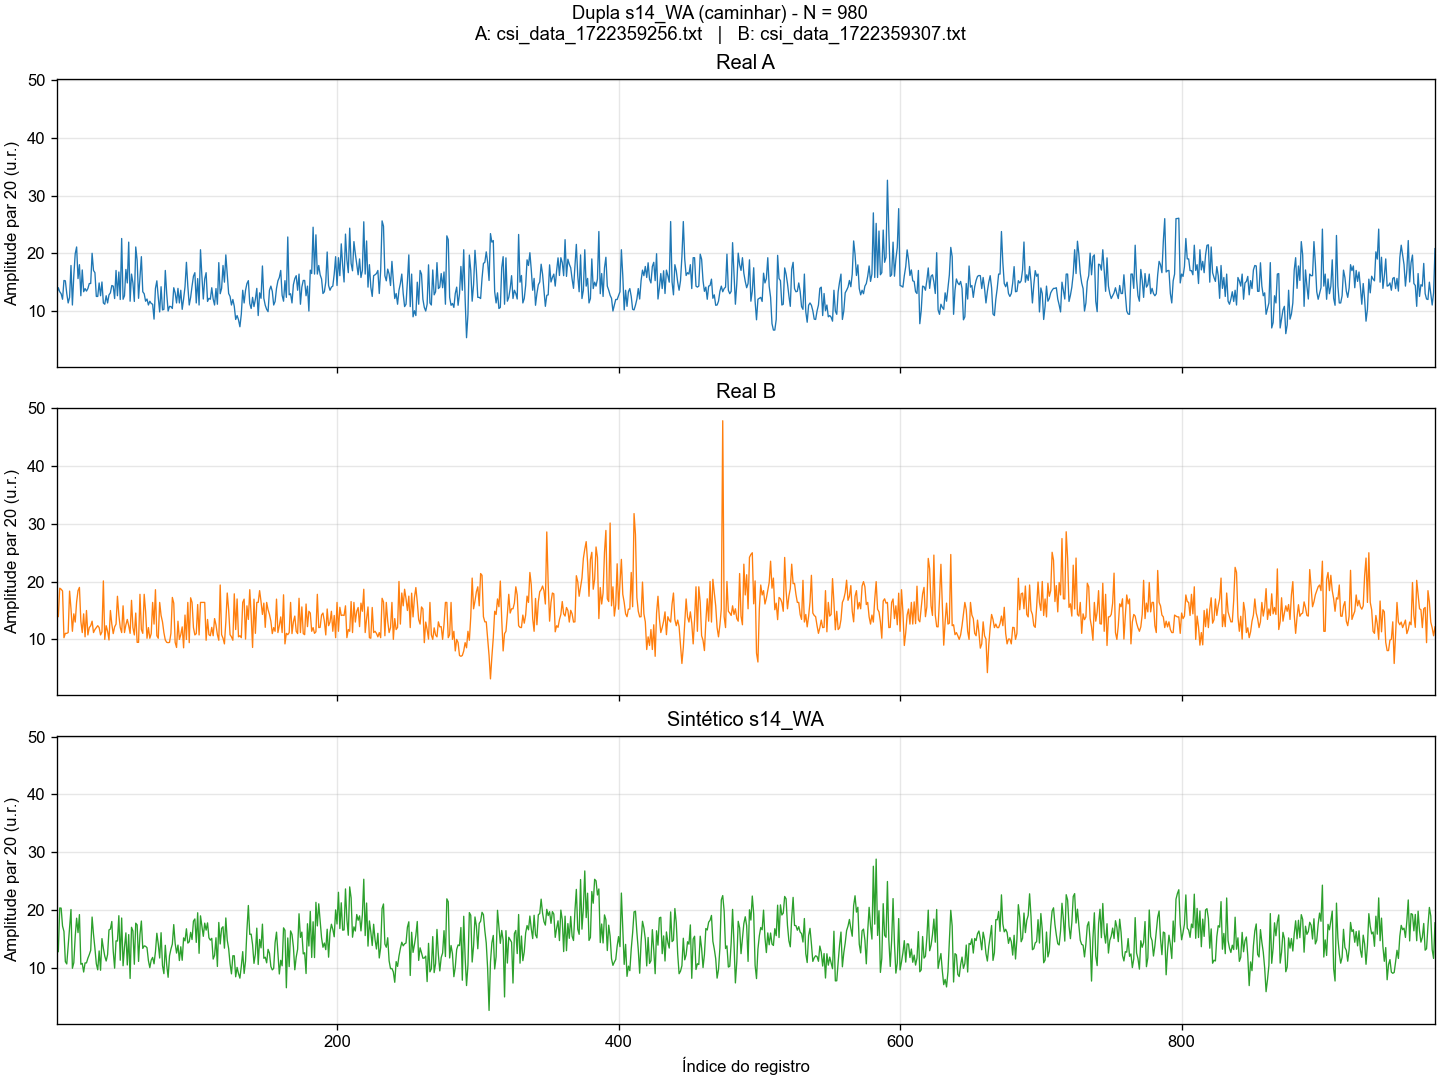
\includegraphics[width=0.79\textwidth,height=19.0cm,keepaspectratio]{Imagens/sec5_comparacao_s14_WA.png}
    \caption{Dupla s14\_WA: Real A (csi\_data\_1722359256.txt), Real B (csi\_data\_1722359307.txt) e Sintético s14\_WA, N = 980. (arquivo: figuras/sec5\_comparacao\_s14\_WA.png)}
    \label{fig:sec5_comparacao_s14_WA}
\end{figure}

\subsection{Características dos sinais comparados}

As cinco características foram recalculadas para real\_A, real\_B e sintético usando os mesmos N valores (45 linhas em \textbf{caracteristicas\_emd.csv}; tabela completa no Anexo, Tabela A2). Para cada característica, a tabela abaixo conta em quantas das 15 duplas o valor do sintético ficou entre os valores de A e B, acima ou abaixo, e o afastamento relativo médio em relação à média de A e B.

{\footnotesize
\begin{longtable}{|>{\centering\arraybackslash}p{3.24cm}|>{\centering\arraybackslash}p{1.62cm}|>{\centering\arraybackslash}p{1.30cm}|>{\centering\arraybackslash}p{1.30cm}|>{\centering\arraybackslash}p{2.60cm}|>{\centering\arraybackslash}p{3.24cm}|}
\caption{Posição das características do sinal sintético em relação a A e B (15 duplas).}\\
\hline
\textbf{Característica} & \textbf{Entre A e B} & \textbf{Acima} & \textbf{Abaixo} & \textbf{Afastamento médio (\%)} & \textbf{Maior afastamento} \\ \hline
\endfirsthead
\hline
\textbf{Característica} & \textbf{Entre A e B} & \textbf{Acima} & \textbf{Abaixo} & \textbf{Afastamento médio (\%)} & \textbf{Maior afastamento} \\ \hline
\endhead
média & 14 & 1 & 0 & 0,6 & s14\_LD (2,4\%) \\ \hline
mediana & 5 & 9 & 1 & 2,7 & s12\_LD (7,0\%) \\ \hline
desvio padrão & 10 & 2 & 3 & 3,4 & s14\_LD (7,3\%) \\ \hline
amplitude pico a pico & 6 & 6 & 3 & 12,0 & s13\_SD (28,9\%) \\ \hline
média das dif. absolutas & 5 & 10 & 0 & 7,5 & s13\_SD (14,5\%) \\ \hline
\end{longtable}
}

{\footnotesize
\begin{longtable}{|>{\centering\arraybackslash}p{1.72cm}|>{\centering\arraybackslash}p{2.27cm}|>{\centering\arraybackslash}p{2.27cm}|>{\centering\arraybackslash}p{2.27cm}|>{\centering\arraybackslash}p{2.27cm}|>{\centering\arraybackslash}p{2.50cm}|}
\caption{Comparação dupla a dupla: posição de cada característica do sinal sintético em relação à faixa [menor, maior] dos valores de A e B. Entre parênteses, quanto o sintético passou do limite mais próximo; em negrito, afastamentos maiores que 5\% (considerados diferentes). Valores completos na Tabela A2.}\\
\hline
\textbf{Dupla} & \textbf{média} & \textbf{mediana} & \textbf{desvio padrão} & \textbf{pico a pico} & \textbf{dif. absolutas} \\ \hline
\endfirsthead
\hline
\textbf{Dupla} & \textbf{média} & \textbf{mediana} & \textbf{desvio padrão} & \textbf{pico a pico} & \textbf{dif. absolutas} \\ \hline
\endhead
s12\_FA & dentro & acima (+1,6\%) & dentro & \textbf{acima (+10,4\%)} & dentro \\ \hline
s12\_GU & dentro & \textbf{acima (+5,6\%)} & dentro & \textbf{acima (+12,0\%)} & dentro \\ \hline
s12\_LD & dentro & \textbf{acima (+5,7\%)} & dentro & dentro & dentro \\ \hline
s12\_SD & dentro & dentro & dentro & dentro & acima (+3,6\%) \\ \hline
s12\_WA & dentro & acima (+1,5\%) & dentro & \textbf{acima (+9,7\%)} & \textbf{acima (+6,8\%)} \\ \hline
s13\_FA & dentro & dentro & abaixo (-4,7\%) & \textbf{abaixo (-19,7\%)} & \textbf{acima (+5,8\%)} \\ \hline
s13\_GU & dentro & dentro & \textbf{abaixo (-5,5\%)} & dentro & dentro \\ \hline
s13\_LD & dentro & dentro & abaixo (-2,1\%) & dentro & dentro \\ \hline
s13\_SD & dentro & acima (+0,8\%) & dentro & \textbf{abaixo (-22,9\%)} & \textbf{acima (+11,4\%)} \\ \hline
s13\_WA & dentro & abaixo (-0,3\%) & acima (+2,4\%) & acima (+4,1\%) & \textbf{acima (+5,3\%)} \\ \hline
s14\_FA & dentro & acima (+2,4\%) & dentro & dentro & \textbf{acima (+6,9\%)} \\ \hline
s14\_GU & dentro & dentro & acima (+1,9\%) & \textbf{acima (+17,7\%)} & \textbf{acima (+13,8\%)} \\ \hline
s14\_LD & dentro & acima (+1,0\%) & dentro & dentro & acima (+3,7\%) \\ \hline
s14\_SD & dentro & acima (+1,2\%) & dentro & \textbf{acima (+10,9\%)} & \textbf{acima (+12,1\%)} \\ \hline
s14\_WA & acima (+0,2\%) & acima (+3,6\%) & dentro & abaixo (-3,9\%) & acima (+2,9\%) \\ \hline
\end{longtable}
}

\subsection{Interpretação}

\textbf{1. Comportamentos das séries reais que aparecem no sintético.} O nível médio e a textura da oscilação rápida são preservados em todas as duplas. Exemplos com trechos identificáveis: em \textbf{s12\_LD} (Figura 14), os picos de até 157 da série B nos registros $\sim$1-250 reaparecem no sintético nos mesmos índices, mas atenuados (máximo 79,3), porque a IMF1 - que concentra os picos - veio de A, que não tem picos; apenas a parte dos picos presente nas IMFs 2, 4 e 6 de B foi transferida. Em \textbf{s13\_LD} (Figura 19), o sintético mostra maior variação nos registros $\sim$1-200 e um vale perto do registro 145, combinando a perturbação inicial de B (registros $\sim$1-150) e, em menor grau, a de A (registros $\sim$200-280). Em \textbf{s13\_WA} (Figura 21), os surtos quase periódicos das séries reais aparecem também no sintético (por exemplo, perto dos registros 60, 360 e 670). Em \textbf{s14\_SD} (Figura 25), as duas gravações têm a maior perturbação nos registros $\sim$280-370 e ficam estáveis depois do registro $\sim$400; o sintético reproduz essa estrutura (pico de 36,7 perto do registro 300 e trecho estável depois de $\sim$400) porque o evento ocorre em posições parecidas em A e B. Quando os eventos não coincidem no tempo, como em s13\_LD, o sintético mistura trechos de movimento e de repouso.

\textbf{2. Características do sintético em relação a A e B.} A \textbf{média} ficou entre A e B em 14 das 15 duplas (afastamento médio de 0,6\%); a exceção é s14\_WA, ligeiramente acima (14,90 contra 14,87 e 14,66). Isso é esperado, pois as IMFs têm média próxima de zero e o nível vem da média dos resíduos. O \textbf{desvio padrão} ficou entre A e B em 10 duplas e próximo nas demais (afastamento médio de 3,4\%). A \textbf{mediana} tende a ficar acima (9 duplas), indicando uma distribuição um pouco mais simétrica que a das séries reais. A \textbf{média das diferenças absolutas} ficou acima de A e B em 10 duplas (por exemplo, s13\_SD: 3,04 contra 2,58 e 2,73; s14\_GU: 4,45 contra 3,91 e 3,91): ao somar IMFs vizinhas de gravações independentes, perde-se a coerência de fase entre elas e o sinal fica mais 'rugoso'. O \textbf{pico a pico} é o menos preservado (afastamento médio de 12\%), por depender de valores extremos isolados: em s13\_SD caiu para 25,25 (A 38,29, B 32,73), e em s14\_GU subiu para 40,37 (A 33,12, B 34,30). A Tabela 8 mostra a comparação dupla a dupla, resumida abaixo (critério: próxima = dentro da faixa de A e B ou até 5\% além dela; diferente = mais de 5\% além da faixa; valores completos na Tabela A2):

\begin{itemize}
    \item \textbf{s12\_FA}: próximas em média, mediana, desvio padrão, dif. absolutas; diferente em pico a pico (sintético 28,87 contra A 26,14 e B 24,90, acima da faixa).
    \item \textbf{s12\_GU}: próximas em média, desvio padrão, dif. absolutas; diferentes em mediana (sintético 28,06 contra A 26,17 e B 26,57, acima da faixa); pico a pico (sintético 33,27 contra A 29,70 e B 29,70, acima da faixa).
    \item \textbf{s12\_LD}: próximas em média, desvio padrão, pico a pico, dif. absolutas; diferente em mediana (sintético 27,66 contra A 26,17 e B 25,55, acima da faixa).
    \item \textbf{s12\_SD}: as cinco características ficaram próximas de A e B.
    \item \textbf{s12\_WA}: próximas em média, mediana, desvio padrão; diferentes em pico a pico (sintético 34,23 contra A 29,58 e B 31,21, acima da faixa); dif. absolutas (sintético 5,63 contra A 5,27 e B 4,99, acima da faixa).
    \item \textbf{s13\_FA}: próximas em média, mediana, desvio padrão; diferentes em pico a pico (sintético 16,80 contra A 23,08 e B 20,93, abaixo da faixa); dif. absolutas (sintético 2,92 contra A 2,76 e B 2,51, acima da faixa).
    \item \textbf{s13\_GU}: próximas em média, mediana, pico a pico, dif. absolutas; diferente em desvio padrão (sintético 5,21 contra A 5,51 e B 5,71, abaixo da faixa).
    \item \textbf{s13\_LD}: as cinco características ficaram próximas de A e B.
    \item \textbf{s13\_SD}: próximas em média, mediana, desvio padrão; diferentes em pico a pico (sintético 25,25 contra A 38,29 e B 32,73, abaixo da faixa); dif. absolutas (sintético 3,04 contra A 2,58 e B 2,73, acima da faixa).
    \item \textbf{s13\_WA}: próximas em média, mediana, desvio padrão, pico a pico; diferente em dif. absolutas (sintético 4,21 contra A 4,00 e B 3,92, acima da faixa).
    \item \textbf{s14\_FA}: próximas em média, mediana, desvio padrão, pico a pico; diferente em dif. absolutas (sintético 3,05 contra A 2,76 e B 2,85, acima da faixa).
    \item \textbf{s14\_GU}: próximas em média, mediana, desvio padrão; diferentes em pico a pico (sintético 40,37 contra A 33,12 e B 34,30, acima da faixa); dif. absolutas (sintético 4,45 contra A 3,91 e B 3,91, acima da faixa).
    \item \textbf{s14\_LD}: as cinco características ficaram próximas de A e B.
    \item \textbf{s14\_SD}: próximas em média, mediana, desvio padrão; diferentes em pico a pico (sintético 31,48 contra A 28,39 e B 27,90, acima da faixa); dif. absolutas (sintético 3,10 contra A 2,76 e B 2,68, acima da faixa).
    \item \textbf{s14\_WA}: as cinco características ficaram próximas de A e B.
\end{itemize}
Em resumo, 4 das 15 duplas tiveram as cinco características próximas das reais. As características que mais vezes ficaram diferentes foram o pico a pico (7 duplas) e a média das diferenças absolutas (7 duplas). A média ficou próxima em todas as duplas; a mediana ficou diferente em 2 duplas e o desvio padrão em 1. Ou seja, o método preserva bem o nível e a dispersão, mas altera os extremos e a rapidez da variação entre registros.

\textbf{3. Valores negativos e fora da faixa.} Surgiram valores negativos em \textbf{2 duplas}: s12\_LD (2 valores, mínimo -2,06), s13\_WA (3 valores, mínimo -1,90). Valores fora da faixa [mínimo, máximo] das séries reais A e B ocorreram em 9 duplas: s12\_FA (8), s12\_GU (11), s12\_LD (32), s12\_WA (10), s13\_WA (7), s14\_GU (7), s14\_LD (6), s14\_SD (1), s14\_WA (1); nas outras 6 duplas o sintético ficou inteiramente dentro da faixa real. Uma amplitude é um módulo e não pode ser negativa: esses valores são artefatos da soma de componentes de gravações diferentes, cujas oscilações negativas deixam de ser compensadas pelas componentes que existiam no sinal original. Eles ocorrem em duplas cujas séries reais já chegam perto de zero (s13\_WA tem mínimo real 1,0) ou têm picos grandes (s12\_LD). Os valores foram \textbf{mantidos sem tratamento}, para registrar fielmente o comportamento do método; para uso em treinamento, uma opção seria limitar os valores a zero ou trabalhar com dados normalizados, como fazem os autores.

\textbf{4. Limitações.}

\begin{itemize}
    \item Apenas o par 20 foi decomposto; o método dos autores trata 52 subportadoras ao mesmo tempo.
    \item Cada sinal sintético vem de só duas gravações, cortadas no mesmo N sem alinhar os instantes dos movimentos; a recombinação pode misturar a fase 'em movimento' de uma gravação com a fase 'parado' da outra.
    \item A EEMD é estocástica: o resultado depende da semente, do número de tentativas e da amplitude do ruído. O erro de reconstrução (desvio de $\sim$0,7 a $\sim$1,6) mostra que as IMFs não somam exatamente o sinal. O número de IMFs é limitado por max\_imf = 7 e, quando as tentativas geram quantidades diferentes de IMFs, a média do ensemble combina componentes diferentes (problema que motivou separate\_trends = True).
    \item O sinal sintético não tem garantia de validade física (valores negativos), e as características usadas são estatísticas de primeira ordem de uma única série.
    \item A semelhança visual ou estatística entre sintético e reais não comprova melhoria no reconhecimento das atividades; isso só pode ser avaliado com um classificador, respeitando a divisão de treino e teste (segunda parte).
\end{itemize}

\section{Conclusões}

\begin{itemize}
    \item A base analisada tem 1.647 gravações de 22 participantes, todas com formato válido, coincidindo com o artigo; os identificadores s18 e s20 não existem e algumas combinações têm 14 ou 16 gravações.
    \item No par 20, o nível da amplitude é dominado pelo participante (e possivelmente pela sessão de coleta), e não pela atividade. As atividades de transição (SD, GU, LD, FA) tendem a ter variação concentrada em um trecho, enquanto WA tem variação distribuída por toda a gravação.
    \item As cinco características se sobrepõem entre atividades e, isoladamente, não separam as cinco classes; o pico a pico é muito sensível a valores extremos e a média das diferenças absolutas diferencia mais os participantes.
    \item Os mapas de calor mostram pares sem informação útil (par 1 constante, par 2 constante, pares 28-38 próximos de zero), coerentes com as subportadoras nulas e piloto removidas pelos autores.
    \item A recombinação de IMFs por EEMD preserva bem o nível e a dispersão dos sinais reais, mas aumenta a variação entre registros consecutivos e pode gerar valores negativos e fora da faixa real. A configuração da EEMD precisou ser ajustada (separate\_trends = True) para evitar que o nível do sinal fosse somado duas vezes - uma fragilidade também presente no código original.
\end{itemize}

\section{Referências}

\begin{itemize}
    \item ARMENTA-GARCIA, J. A.; GONZALEZ-NAVARRO, F. F.; CARO-GUTIERREZ, J.; GARCIA-REYES, C. I. Tools and Methods for Achieving Wi-Fi Sensing in Embedded Devices. \textit{Sensors}, v. 25, 6220, 2025. DOI: 10.3390/s25196220.
    \item Repositório Embedded\_WiFi\_Sensing (arquivo Embedded\_WiFi\_Sensing-main fornecido pelo professor): Scripts/CSI.py, Scripts/imf\_generator.py, Scripts/imf\_sample\_builder.py e Scripts/dataset\_constructor.py.
    \item LASZUK, D. PyEMD: Python implementation of Empirical Mode Decomposition (pacote EMD-signal, versão 1.10.0).
    \item HUANG, N. E. et al. The empirical mode decomposition and the Hilbert spectrum for nonlinear and non-stationary time series analysis. \textit{Proc. R. Soc. Lond. A}, v. 454, p. 903-995, 1998.
    \item WU, Z.; HUANG, N. E. Ensemble empirical mode decomposition: a noise-assisted data analysis method. \textit{Advances in Adaptive Data Analysis}, v. 1, n. 1, p. 1-41, 2009.
\end{itemize}
\newpage

\section*{Anexo - Tabelas completas}
\addcontentsline{toc}{section}{Anexo - Tabelas completas}
\setcounter{table}{0}\renewcommand{\thetable}{A\arabic{table}}

{\footnotesize
\begin{longtable}{|>{\centering\arraybackslash}p{0.76cm}|>{\centering\arraybackslash}p{0.76cm}|>{\centering\arraybackslash}p{2.55cm}|>{\centering\arraybackslash}p{0.76cm}|>{\centering\arraybackslash}p{0.76cm}|>{\centering\arraybackslash}p{1.10cm}|>{\centering\arraybackslash}p{1.10cm}|>{\centering\arraybackslash}p{1.10cm}|>{\centering\arraybackslash}p{1.24cm}|>{\centering\arraybackslash}p{1.38cm}|}
\caption{Características da série completa do par 20 das 30 gravações (caracteristicas\_reais.csv; caminho: Datasets/Activity/\textless{}ativ.\textgreater{}/\textless{}part.\textgreater{}/\textless{}arquivo\textgreater{}).}\\
\hline
\textbf{Part.} & \textbf{Ativ.} & \textbf{Arquivo TXT} & \textbf{Ordem} & \textbf{N} & \textbf{Média} & \textbf{Mediana} & \textbf{Desvio} & \textbf{Pico a pico} & \textbf{Média dif. abs.} \\ \hline
\endfirsthead
\hline
\textbf{Part.} & \textbf{Ativ.} & \textbf{Arquivo TXT} & \textbf{Ordem} & \textbf{N} & \textbf{Média} & \textbf{Mediana} & \textbf{Desvio} & \textbf{Pico a pico} & \textbf{Média dif. abs.} \\ \hline
\endhead
s12 & FA & csi\_data\_1722274497.txt & 1 & 974 & 26,7176 & 26,1725 & 4,7789 & 26,1429 & 5,1053 \\ \hline
s12 & FA & csi\_data\_1722274542.txt & 2 & 963 & 27,2490 & 25,7099 & 5,2940 & 24,9025 & 5,5351 \\ \hline
s12 & GU & csi\_data\_1722275364.txt & 1 & 987 & 27,5514 & 26,1725 & 5,3709 & 29,6965 & 5,2425 \\ \hline
s12 & GU & csi\_data\_1722275473.txt & 2 & 990 & 28,9887 & 26,5989 & 6,4494 & 29,6965 & 6,7637 \\ \hline
s12 & LD & csi\_data\_1722275315.txt & 1 & 991 & 28,1107 & 26,2488 & 5,2515 & 27,5078 & 5,1991 \\ \hline
s12 & LD & csi\_data\_1722275426.txt & 2 & 936 & 29,0426 & 25,5539 & 11,1062 & 140,6338 & 7,7361 \\ \hline
s12 & SD & csi\_data\_1722273691.txt & 1 & 976 & 26,8031 & 26,1725 & 5,1398 & 33,5245 & 4,6664 \\ \hline
s12 & SD & csi\_data\_1722273739.txt & 2 & 978 & 29,7026 & 29,1548 & 5,4391 & 30,0109 & 4,9441 \\ \hline
s12 & WA & csi\_data\_1722272856.txt & 1 & 995 & 25,1674 & 24,1661 & 5,7411 & 29,5793 & 5,2670 \\ \hline
s12 & WA & csi\_data\_1722272903.txt & 2 & 994 & 25,2294 & 24,3413 & 5,5974 & 31,2120 & 4,9860 \\ \hline
s13 & FA & csi\_data\_1722285593.txt & 1 & 987 & 10,4454 & 10,1980 & 3,0099 & 23,0832 & 2,7864 \\ \hline
s13 & FA & csi\_data\_1722285652.txt & 2 & 978 & 9,1762 & 8,9443 & 3,0272 & 20,9317 & 2,5061 \\ \hline
s13 & GU & csi\_data\_1722281824.txt & 1 & 962 & 26,9455 & 25,5539 & 5,5116 & 36,8767 & 5,2542 \\ \hline
s13 & GU & csi\_data\_1722281947.txt & 2 & 986 & 27,2341 & 27,7669 & 5,7137 & 25,7888 & 5,9442 \\ \hline
s13 & LD & csi\_data\_1722281718.txt & 1 & 979 & 28,6712 & 29,6816 & 5,4972 & 38,2332 & 4,8719 \\ \hline
s13 & LD & csi\_data\_1722281887.txt & 2 & 983 & 28,2861 & 28,0713 & 6,1100 & 31,0795 & 6,3948 \\ \hline
s13 & SD & csi\_data\_1722286503.txt & 1 & 992 & 12,7686 & 12,0416 & 4,1990 & 38,2884 & 2,5788 \\ \hline
s13 & SD & csi\_data\_1722286550.txt & 2 & 991 & 13,3036 & 12,6491 & 3,5051 & 32,7343 & 2,7286 \\ \hline
s13 & WA & csi\_data\_1722284702.txt & 1 & 982 & 13,0844 & 12,7279 & 5,6810 & 33,9285 & 4,0136 \\ \hline
s13 & WA & csi\_data\_1722284759.txt & 2 & 975 & 13,5165 & 13,1529 & 5,7122 & 30,9531 & 3,9206 \\ \hline
s14 & FA & csi\_data\_1722360030.txt & 1 & 974 & 15,5877 & 14,8661 & 3,0144 & 20,2573 & 2,7636 \\ \hline
s14 & FA & csi\_data\_1722360079.txt & 2 & 992 & 15,4181 & 14,5602 & 3,1652 & 22,6274 & 2,8513 \\ \hline
s14 & GU & csi\_data\_1722361809.txt & 1 & 986 & 22,0375 & 22,2036 & 6,8430 & 33,1204 & 3,9126 \\ \hline
s14 & GU & csi\_data\_1722361907.txt & 2 & 994 & 21,8005 & 20,6155 & 6,6954 & 34,3040 & 3,9006 \\ \hline
s14 & LD & csi\_data\_1722361762.txt & 1 & 983 & 17,4815 & 16,4012 & 3,8698 & 20,0333 & 3,5918 \\ \hline
s14 & LD & csi\_data\_1722361861.txt & 2 & 990 & 18,6168 & 17,2627 & 4,7183 & 24,3510 & 3,7263 \\ \hline
s14 & SD & csi\_data\_1722360869.txt & 1 & 989 & 15,2859 & 14,2127 & 3,9984 & 28,3886 & 2,7547 \\ \hline
s14 & SD & csi\_data\_1722360914.txt & 2 & 977 & 14,6788 & 13,9284 & 3,6845 & 27,9022 & 2,6789 \\ \hline
s14 & WA & csi\_data\_1722359256.txt & 1 & 991 & 14,9040 & 14,4222 & 3,5609 & 27,2645 & 2,9513 \\ \hline
s14 & WA & csi\_data\_1722359307.txt & 2 & 980 & 14,6621 & 14,2127 & 3,9223 & 44,6917 & 3,1636 \\ \hline
\end{longtable}
}

\newpage

{\footnotesize
\begin{longtable}{|>{\centering\arraybackslash}p{1.44cm}|>{\centering\arraybackslash}p{1.52cm}|>{\centering\arraybackslash}p{0.96cm}|>{\centering\arraybackslash}p{1.60cm}|>{\centering\arraybackslash}p{1.60cm}|>{\centering\arraybackslash}p{1.60cm}|>{\centering\arraybackslash}p{1.76cm}|>{\centering\arraybackslash}p{1.92cm}|}
\caption{Características das 45 séries comparadas (caracteristicas\_emd.csv). Arquivos A e B de cada dupla: ver Tabela 6.}\\
\hline
\textbf{Dupla} & \textbf{Tipo} & \textbf{N} & \textbf{Média} & \textbf{Mediana} & \textbf{Desvio} & \textbf{Pico a pico} & \textbf{Média dif. abs.} \\ \hline
\endfirsthead
\hline
\textbf{Dupla} & \textbf{Tipo} & \textbf{N} & \textbf{Média} & \textbf{Mediana} & \textbf{Desvio} & \textbf{Pico a pico} & \textbf{Média dif. abs.} \\ \hline
\endhead
s12\_FA & real\_A & 963 & 26,7155 & 26,1725 & 4,7801 & 26,1429 & 5,0862 \\ \hline
s12\_FA & real\_B & 963 & 27,2490 & 25,7099 & 5,2940 & 24,9025 & 5,5351 \\ \hline
s12\_FA & sintetico & 963 & 26,9081 & 26,5990 & 4,9387 & 28,8745 & 5,4499 \\ \hline
s12\_GU & real\_A & 987 & 27,5514 & 26,1725 & 5,3709 & 29,6965 & 5,2425 \\ \hline
s12\_GU & real\_B & 987 & 28,9914 & 26,5707 & 6,4583 & 29,6965 & 6,7761 \\ \hline
s12\_GU & sintetico & 987 & 28,4707 & 28,0551 & 5,6986 & 33,2709 & 5,7515 \\ \hline
s12\_LD & real\_A & 936 & 28,1105 & 26,1725 & 5,2822 & 27,5078 & 5,2785 \\ \hline
s12\_LD & real\_B & 936 & 29,0426 & 25,5539 & 11,1062 & 140,6338 & 7,7361 \\ \hline
s12\_LD & sintetico & 936 & 28,4163 & 27,6629 & 8,3854 & 81,3037 & 6,8783 \\ \hline
s12\_SD & real\_A & 976 & 26,8031 & 26,1725 & 5,1398 & 33,5245 & 4,6664 \\ \hline
s12\_SD & real\_B & 976 & 29,7015 & 29,1548 & 5,4394 & 30,0109 & 4,9357 \\ \hline
s12\_SD & sintetico & 976 & 28,1531 & 27,8759 & 5,2963 & 30,8791 & 5,1132 \\ \hline
s12\_WA & real\_A & 994 & 25,1676 & 24,1661 & 5,7440 & 29,5793 & 5,2720 \\ \hline
s12\_WA & real\_B & 994 & 25,2294 & 24,3413 & 5,5974 & 31,2120 & 4,9860 \\ \hline
s12\_WA & sintetico & 994 & 25,1899 & 24,7165 & 5,7041 & 34,2275 & 5,6310 \\ \hline
s13\_FA & real\_A & 978 & 10,4338 & 10,1980 & 3,0074 & 23,0832 & 2,7620 \\ \hline
s13\_FA & real\_B & 978 & 9,1762 & 8,9443 & 3,0272 & 20,9317 & 2,5061 \\ \hline
s13\_FA & sintetico & 978 & 9,7182 & 9,4310 & 2,8653 & 16,8002 & 2,9226 \\ \hline
s13\_GU & real\_A & 962 & 26,9455 & 25,5539 & 5,5116 & 36,8767 & 5,2542 \\ \hline
s13\_GU & real\_B & 962 & 27,2632 & 27,8568 & 5,7062 & 25,7888 & 5,9368 \\ \hline
s13\_GU & sintetico & 962 & 27,1472 & 26,5163 & 5,2095 & 31,3486 & 5,6119 \\ \hline
s13\_LD & real\_A & 979 & 28,6712 & 29,6816 & 5,4972 & 38,2332 & 4,8719 \\ \hline
s13\_LD & real\_B & 979 & 28,2789 & 28,0713 & 6,1069 & 31,0795 & 6,3870 \\ \hline
s13\_LD & sintetico & 979 & 28,5607 & 28,7739 & 5,3817 & 33,7426 & 5,4436 \\ \hline
s13\_SD & real\_A & 991 & 12,7700 & 12,0416 & 4,2009 & 38,2884 & 2,5810 \\ \hline
s13\_SD & real\_B & 991 & 13,3036 & 12,6491 & 3,5051 & 32,7343 & 2,7286 \\ \hline
s13\_SD & sintetico & 991 & 13,1027 & 12,7543 & 3,7447 & 25,2489 & 3,0404 \\ \hline
s13\_WA & real\_A & 975 & 13,0944 & 12,7279 & 5,6899 & 33,9285 & 4,0001 \\ \hline
s13\_WA & real\_B & 975 & 13,5165 & 13,1529 & 5,7122 & 30,9531 & 3,9206 \\ \hline
s13\_WA & sintetico & 975 & 13,1391 & 12,6956 & 5,8480 & 35,3123 & 4,2132 \\ \hline
s14\_FA & real\_A & 974 & 15,5877 & 14,8661 & 3,0144 & 20,2573 & 2,7636 \\ \hline
s14\_FA & real\_B & 974 & 15,4211 & 14,5602 & 3,1765 & 22,6274 & 2,8504 \\ \hline
s14\_FA & sintetico & 974 & 15,5414 & 15,2245 & 3,0525 & 20,3780 & 3,0468 \\ \hline
s14\_GU & real\_A & 986 & 22,0375 & 22,2036 & 6,8430 & 33,1204 & 3,9126 \\ \hline
s14\_GU & real\_B & 986 & 21,7154 & 20,5913 & 6,6504 & 34,3040 & 3,9071 \\ \hline
s14\_GU & sintetico & 986 & 21,7432 & 21,4510 & 6,9760 & 40,3710 & 4,4542 \\ \hline
s14\_LD & real\_A & 983 & 17,4815 & 16,4012 & 3,8698 & 20,0333 & 3,5918 \\ \hline
s14\_LD & real\_B & 983 & 18,5956 & 17,2627 & 4,7184 & 24,3510 & 3,7186 \\ \hline
s14\_LD & sintetico & 983 & 17,6041 & 17,4308 & 3,9806 & 23,9258 & 3,8562 \\ \hline
s14\_SD & real\_A & 977 & 15,3101 & 14,3178 & 4,0133 & 28,3886 & 2,7642 \\ \hline
s14\_SD & real\_B & 977 & 14,6788 & 13,9284 & 3,6845 & 27,9022 & 2,6789 \\ \hline
s14\_SD & sintetico & 977 & 15,0540 & 14,4938 & 4,0109 & 31,4776 & 3,0992 \\ \hline
s14\_WA & real\_A & 980 & 14,8700 & 14,3178 & 3,5433 & 27,2645 & 2,9369 \\ \hline
s14\_WA & real\_B & 980 & 14,6621 & 14,2127 & 3,9223 & 44,6917 & 3,1636 \\ \hline
s14\_WA & sintetico & 980 & 14,8990 & 14,8386 & 3,7063 & 26,2006 & 3,2549 \\ \hline
\end{longtable}
}


\end{document}
